\chapter{Erklärung der grundlegenden Benutzeroberfläche}

\section{Bedeutung der Symbole}
\label{sec:icon_list}

Die Benutzeroberfläche (UI) von ToM ist sehr intuitiv und einfach zu bedienen, und jede Angabe wird durch ein spezifisches Symbol dargestellt, das normalerweise darauf hinweist, wofür diese Daten nützlich sein können. Hier ist eine Liste aller Symbole, die Sie auf dem ToM finden könnten, und deren Bedeutung.

\subsection{Seitensymbole}
\label{sec:page_icon_list}

Seitensymbole sind die Symbole, die Sie in der unteren Zeile des ToM+ Displays finden, und sie werden verwendet, um zwischen den verschiedenen Seiten zu wechseln. Seit dem letzten Update wurden sie mit einem metallischen 3D-Look überarbeitet.

\iconbox{icons/BatteryV2.png}
{Batterieseite}
{Zeigt die wichtigsten Werte der Batterie an.}

\iconbox{icons/Motor.png}
{Motorseite}
{Zeigt die wichtigsten Werte des Motors an.}

\iconbox{icons/BatteryInfo2.png}
{Batterie-Info-Seite}
{Zeigt detaillierte Informationen über die Batteriezellen an.}

\iconbox{icons/Alarm.PNG}
{Alarmprotokoll-Seite}
{Zeigt die Liste der letzten Alarmauslöser und deren Details an.}

\iconbox{icons/Error.png}
{Fehlerprotokoll-Seite}
{Zeigt die Liste der letzten Fehler und deren Details an.}

\iconbox{icons/TripLog.png}
{Fahrtprotokoll-Seite}
{Zeigt die Liste der letzten Fahrten und deren Details an.}

\iconbox{icons/Gyroscope.png}
{Gyroskop-Seite}
{Zeigt die wichtigsten Werte des Gyroskops und Verschiedenes an.}

\iconbox{icons/Street0Ok_v2.png}
{Fahrt-Seite}
{Zeigt die wichtigsten Werte der ausgewählten Fahrt an.}

\iconbox{icons/3Dots.PNG}
{Einstellungsseite}
{Zeigt verschiedene Einstellungen und Optionen für das ToM+ an.}

\subsection{Batteriegruppe}
\label{sec:item_numbers}

\iconbox{icons/BatterySoc.jpg}
{(1) Ladezustand (State Of Charge) (\%)}
{Der aktuelle Ladezustand der Batterie.}

\iconbox{icons/BatterySoh.jpg}
{(2) Gesundheitszustand (State Of Health) (\%)}
{Der aktuelle Gesundheitszustand der Batterie.}

\iconbox{icons/BatteryKwh.jpg}
{(6) Verbleibende Batteriekapazität (\(kWh\))}
{Die verbleibende, in der Batterie gespeicherte Energie.}

\iconbox{icons/BatteryA.jpg}
{(7) Aktueller Batteriestromverbrauch (\(A\))}
{Der Strom, der durch die Batterie fließt.}

\iconbox{icons/BatteryA+red.png}
{(7) Batterieladestrom (\(A\))}
{Der Ladestrom durch regeneratives Bremsen.}

\iconbox{icons/BatteryKw.png}
{(54) Momentane Batterieleistung (\(kW\))}
{Die durch die Batterie fließende Leistung.}

\iconbox{icons/Battery3°.jpg}
{(3) Batterietemperatur (\textdegree~C)}
{Die aktuelle Temperatur der Batterie.}

\iconbox{icons/BatteryV2.jpg}
{(25) Batteriespannung (\(V\))}
{Die aktuelle Spannung der Traktionsbatterie.}

\iconbox{icons/BatteryV.jpg}
{(39) 12V Batteriespannung (\(V\))}
{Die aktuelle Spannung der 12V Batterie.}

\iconbox{icons/BatteryDiff.png}
{(5) Min-Max Batteriezellen-Differenz (\(V\))}
{Die Differenz zwischen der minimalen und maximalen Batteriezellenspannung.}

\subsection{Ladegruppe}

\iconbox{icons/CEta.png}
{(55) Lade-ETA (Geschätzte Dauer) (\(min\))}
{Die geschätzte verbleibende Zeit, bis die Batterie vollständig aufgeladen ist.}

\iconbox{icons/Charge°.png}
{(57) Ladegerättemperatur (\textdegree~C)}
{Die aktuelle Temperatur des Ladegeräts.}

\iconbox{icons/ChargedKwh.png}
{(56) Geladene Energie (\(kWh\))}
{Die Energiemenge, die in die Batterie geladen wurde.}

\iconbox{icons/ChargeKwh.png}
{(58) Momentane Ladeleistung (\(kW\))}
{Die aktuelle Leistung, die der Batterie zugeführt wird.}

\subsection{Motorgruppe}

\iconbox{icons/MotoRPM2.jpg}
{(8) Motordrehzahl (\(rpm\))}
{Die aktuellen Umdrehungen pro Minute des Motors.}

\iconbox{icons/MotorNm.jpg}
{(9) Motordrehmoment (\(Nm\))}
{Das aktuelle vom Motor erzeugte Drehmoment.}

\iconbox{icons/Motor°2.jpg}
{(4) Motortemperatur (\textdegree~C)}
{Die aktuelle Temperatur des Motors.}

\iconbox{icons/Sev°.png}
{(45) Sevcon-Temperatur (\textdegree~C)}
{Die aktuelle Temperatur des Sevcon-Controllers.}

\subsection{Erweiterungsport-Gruppe}

\iconbox{icons/Pin1.png}
{(40) Erweiterungsport PIN1 (\(0/1\))}
{Der binäre Zustand des Erweiterungsports PIN1.}

\iconbox{icons/Pin2.png}
{(41) Erweiterungsport PIN2 (\(0/1\))}
{Der binäre Zustand des Erweiterungsports PIN2.}

\subsection{Gyroskopgruppe}

\iconbox{icons/InclDX.PNG}
{(62) Gyroskop rechte X-Achse (\textdegree)}
{Der aktuelle rechte Winkel des Gyroskops entlang der X-Achse.}

\iconbox{icons/InclSX.PNG}
{(62) Gyroskop linke X-Achse (\textdegree)}
{Der aktuelle linke Winkel des Gyroskops entlang der X-Achse.}

\iconbox{icons/UphillTwizy.png}
{(63) Frontale Steigungsneigung (\textdegree)}
{Der aktuelle frontale Steigungswinkel des Gyroskops.}

\iconbox{icons/DownhillTwizy.png}
{(63) Frontale Gefälleneigung (\textdegree)}
{Der aktuelle frontale Gefällewinkel des Gyroskops.}

\iconbox{icons/GyroAcc.JPG}
{(61) Gyroskopbeschleunigung (\(m/s^2\))}
{Die aktuelle Fahrzeugbeschleunigung, gemessen vom Gyroskop.}

\iconbox{icons/Gtemp.PNG}
{(60) ToM+ Blackbox-Temperatur (\textdegree~C)}
{Die aktuelle Temperatur der ToM+ Blackbox.}

\iconbox{icons/Timer.PNG}
{(59) Verstrichene Zeit (\(min\))}
{Die aktuelle verstrichene Zeit seit dem Einschalten.}

\subsection{Fahrtgruppe}

\iconbox{icons/tKm.png}
{(46) Fahrstrecke (\(km\))}
{Die aktuell auf der aktuellen Fahrt zurückgelegte Strecke.}

\iconbox{icons/tKmh.png}
{(53) Durchschnittliche Reisegeschwindigkeit (\(km/h\))}
{Die aktuelle Durchschnittsgeschwindigkeit der aktuellen Fahrt.}

\iconbox{icons/tKmR.png}
{(47) Verbleibende Fahrtkilometer (\(km\))}
{Die verbleibende Kilometerreichweite beim aktuellen Fahrtverbrauch.}

\iconbox{icons/tkWh.png}
{(49) Gesamtstromverbrauch der Fahrt (\(kWh\))}
{Der gesamte Stromverbrauch der aktuellen Fahrt.}

\iconbox{icons/tkWh100.png}
{(50) Fahrtstromverbrauch pro 100 Kilometer (\(kWh/100km\))}
{Der aktuelle Stromverbrauch pro 100 Kilometer der aktuellen Fahrt.}

\iconbox{icons/tkWh1min.png}
{(52) Fahrtstromverbrauch pro Minute (\(kWh/min\))}
{Der aktuelle Stromverbrauch pro Minute der aktuellen Fahrt.}

\iconbox{icons/tTimer.png}
{(48) Fahrzeit (\(min\))}
{Die aktuell verstrichene Zeit der aktuellen Fahrt.}

\iconbox{icons/tUphill.png}
{(38) Durchschnittliche Steigungsneigung der Fahrt (\textdegree)}
{Die durchschnittliche Steigungsneigung der aktuellen Fahrt.}

\iconbox{icons/tDownhill.png}
{(38) Durchschnittliche Gefälleneigung der Fahrt (\textdegree)}
{Die durchschnittliche Gefälleneigung der aktuellen Fahrt.}

\subsection{Armaturenbrettgruppe}

\iconbox{icons/ODO.png}
{(42) Kilometerzähler (\(km\))}
{Die vom Fahrzeug insgesamt zurückgelegte Strecke.}

\iconbox{icons/Kmh.png}
{Aktuelle Geschwindigkeit (\(km/h\))}
{(44) Die aktuelle Geschwindigkeit des Fahrzeugs.}

\iconbox{icons/KmhR.png}
{(43) Verbleibende Kilometer (\(km\))}
{Die vom Original-Armaturenbrett berechnete verbleibende Strecke.}

\iconbox{icons/KmRCalc.png}
{(51) Berechnete verbleibende Kilometer (\(km\))}
{Die vom ToM+ mit anpassbarem, gewichtetem Durchschnitt berechneten verbleibenden km.}
\label{fig:calculated_kilometers_left}

\clearpage

\section{Armaturenbrett-Seite}

Dieser Abschnitt befasst sich mit der Erklärung der Armaturenbrett-Seite, die die Hauptseite des ToM+ ist und wahrscheinlich diejenige, die Sie am meisten verwenden werden. Auf dem Bild unten habe ich die wichtigsten Teile nummeriert und werde sie in den folgenden Absätzen erklären.

\begin{figure}[H]
    \centering
    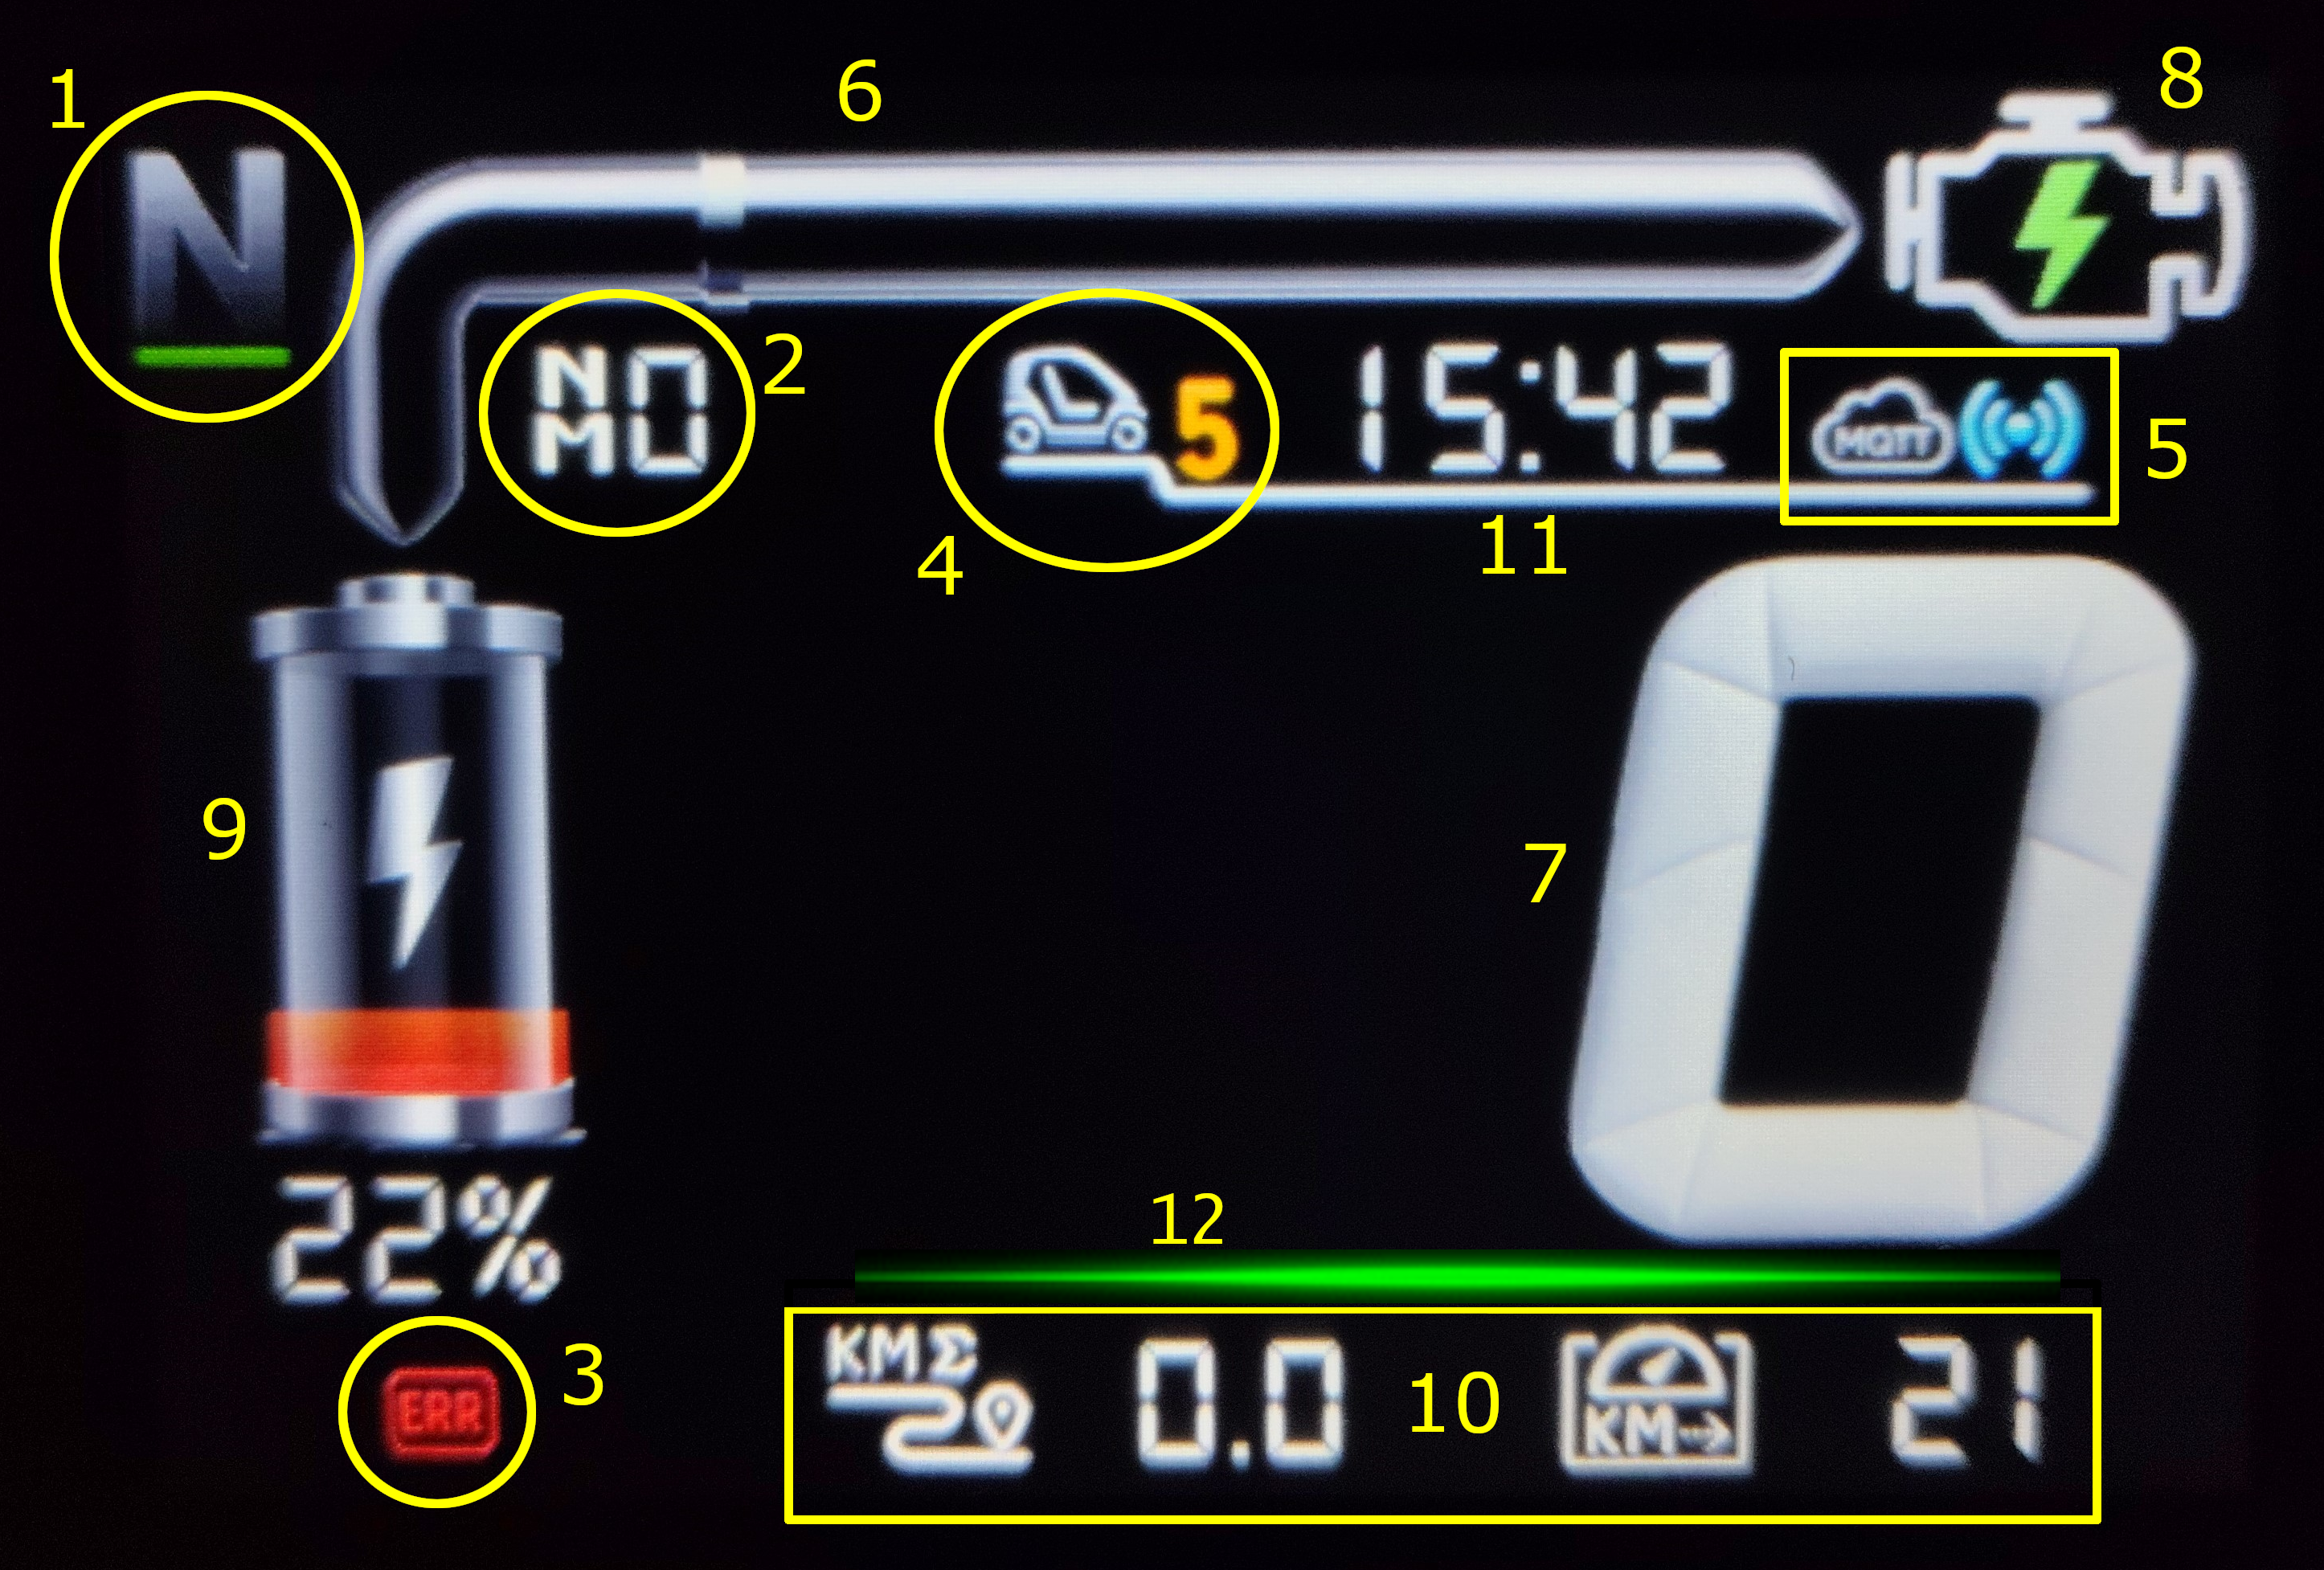
\includegraphics[width=0.8\textwidth]{figures/dashboard_numbers.PNG}
    \caption{Armaturenbrett-Seite mit nummerierten Teilen.} \label{fig:dashboard_layout}
\end{figure}

\begin{description}
\item[\textbf{1}] Aktueller Gang des Fahrzeugs, der normalerweise auch auf dem Original-Armaturenbrett angezeigt wird.
\item[\textbf{2}] Ein Wert, der aus Drehmoment, Stromverbrauch und Stromaufnahme ausgewählt wird und zum Füllen des in Punkt 6 beschriebenen Leistungsbalkens dient. Tippen Sie auf den Wert, um zwischen den drei Optionen zu wechseln.
\item[\textbf{3}] Fehlerstatus-Symbol, wird angezeigt, wenn ein Fehler vorliegt.
\item[\textbf{4}] Zeigt die aktive Fahrt an. Tippen Sie auf das Symbol, um die Fahrt-Seite zu öffnen.
\item[\textbf{5}] Symbole für MQTT und WiFi. Ausgegraut, wenn keine Verbindung besteht, und farbig bei Verbindung. Tippen Sie auf die Symbole, wenn Sie einen neuen WiFi-Scan oder eine MQTT-Neuverbindung durchführen möchten.
\item[\textbf{6}] Leistungsbalken, der den in Punkt 2 ausgewählten Wert anzeigt. Ausgehend von der Mittellinie füllt sich der Balken beim Beschleunigen von links nach rechts und beim regenerativen Bremsen von rechts nach links. Der Balken wird in beide Richtungen mit einem Farbverlauf gefüllt, und die \textbf{Maximal- und Minimalwerte sind anpassbar} auf der BigToM-Seite des Webservers.
\item[\textbf{7}] Zeigt die momentane Geschwindigkeit des Fahrzeugs an. Sie können auf der Webserver-Seite "Erweiterte Info und Einstellungen" zwischen km/h und mph wählen.
\item[\textbf{8}] Motorsymbol, tippen Sie darauf, um die Motorseite zu öffnen.
\item[\textbf{9}] Batterie-Symbol mit Farbverlauf, tippen Sie darauf, um die Batterie-Info-Seite zu öffnen.
\item[\textbf{10}] Zusätzlich angezeigte Werte, Sie können durch Antippen des Symbols zwischen ihnen wechseln.
\item[\textbf{11}] Zeigt Uhrzeit und Datum an, wechseln Sie durch Antippen zwischen ihnen.
\item[\textbf{12}] Anpassbares Geschwindigkeitswarnlimit (grün, gelb oder rot), siehe Abschnitt~\ref{sec:web_btom_tom_sets} zur Aktivierung.
\end{description}

\section{Das Seitenlayout}
\label{sec:main-layout}

Das Layout lässt sich in zwei Hauptteile unterteilen, die wir uns in den nächsten beiden Absätzen genauer ansehen werden. Der erste ist der Datenmonitor, der einige Funktionen bietet, um die im Vordergrund angezeigten Daten aus den in der Seitenleiste aufgelisteten auszuwählen. Der zweite ist die Status-Symbolleiste, die sich normalerweise am unteren Rand der Seite befindet.
Die Batterie-, Motor-, Gyroskop- und Fahrt-Seiten teilen sich das gleiche Layout, wie auf dem Bild gezeigt.

\begin{figure}[H]
    \centering
    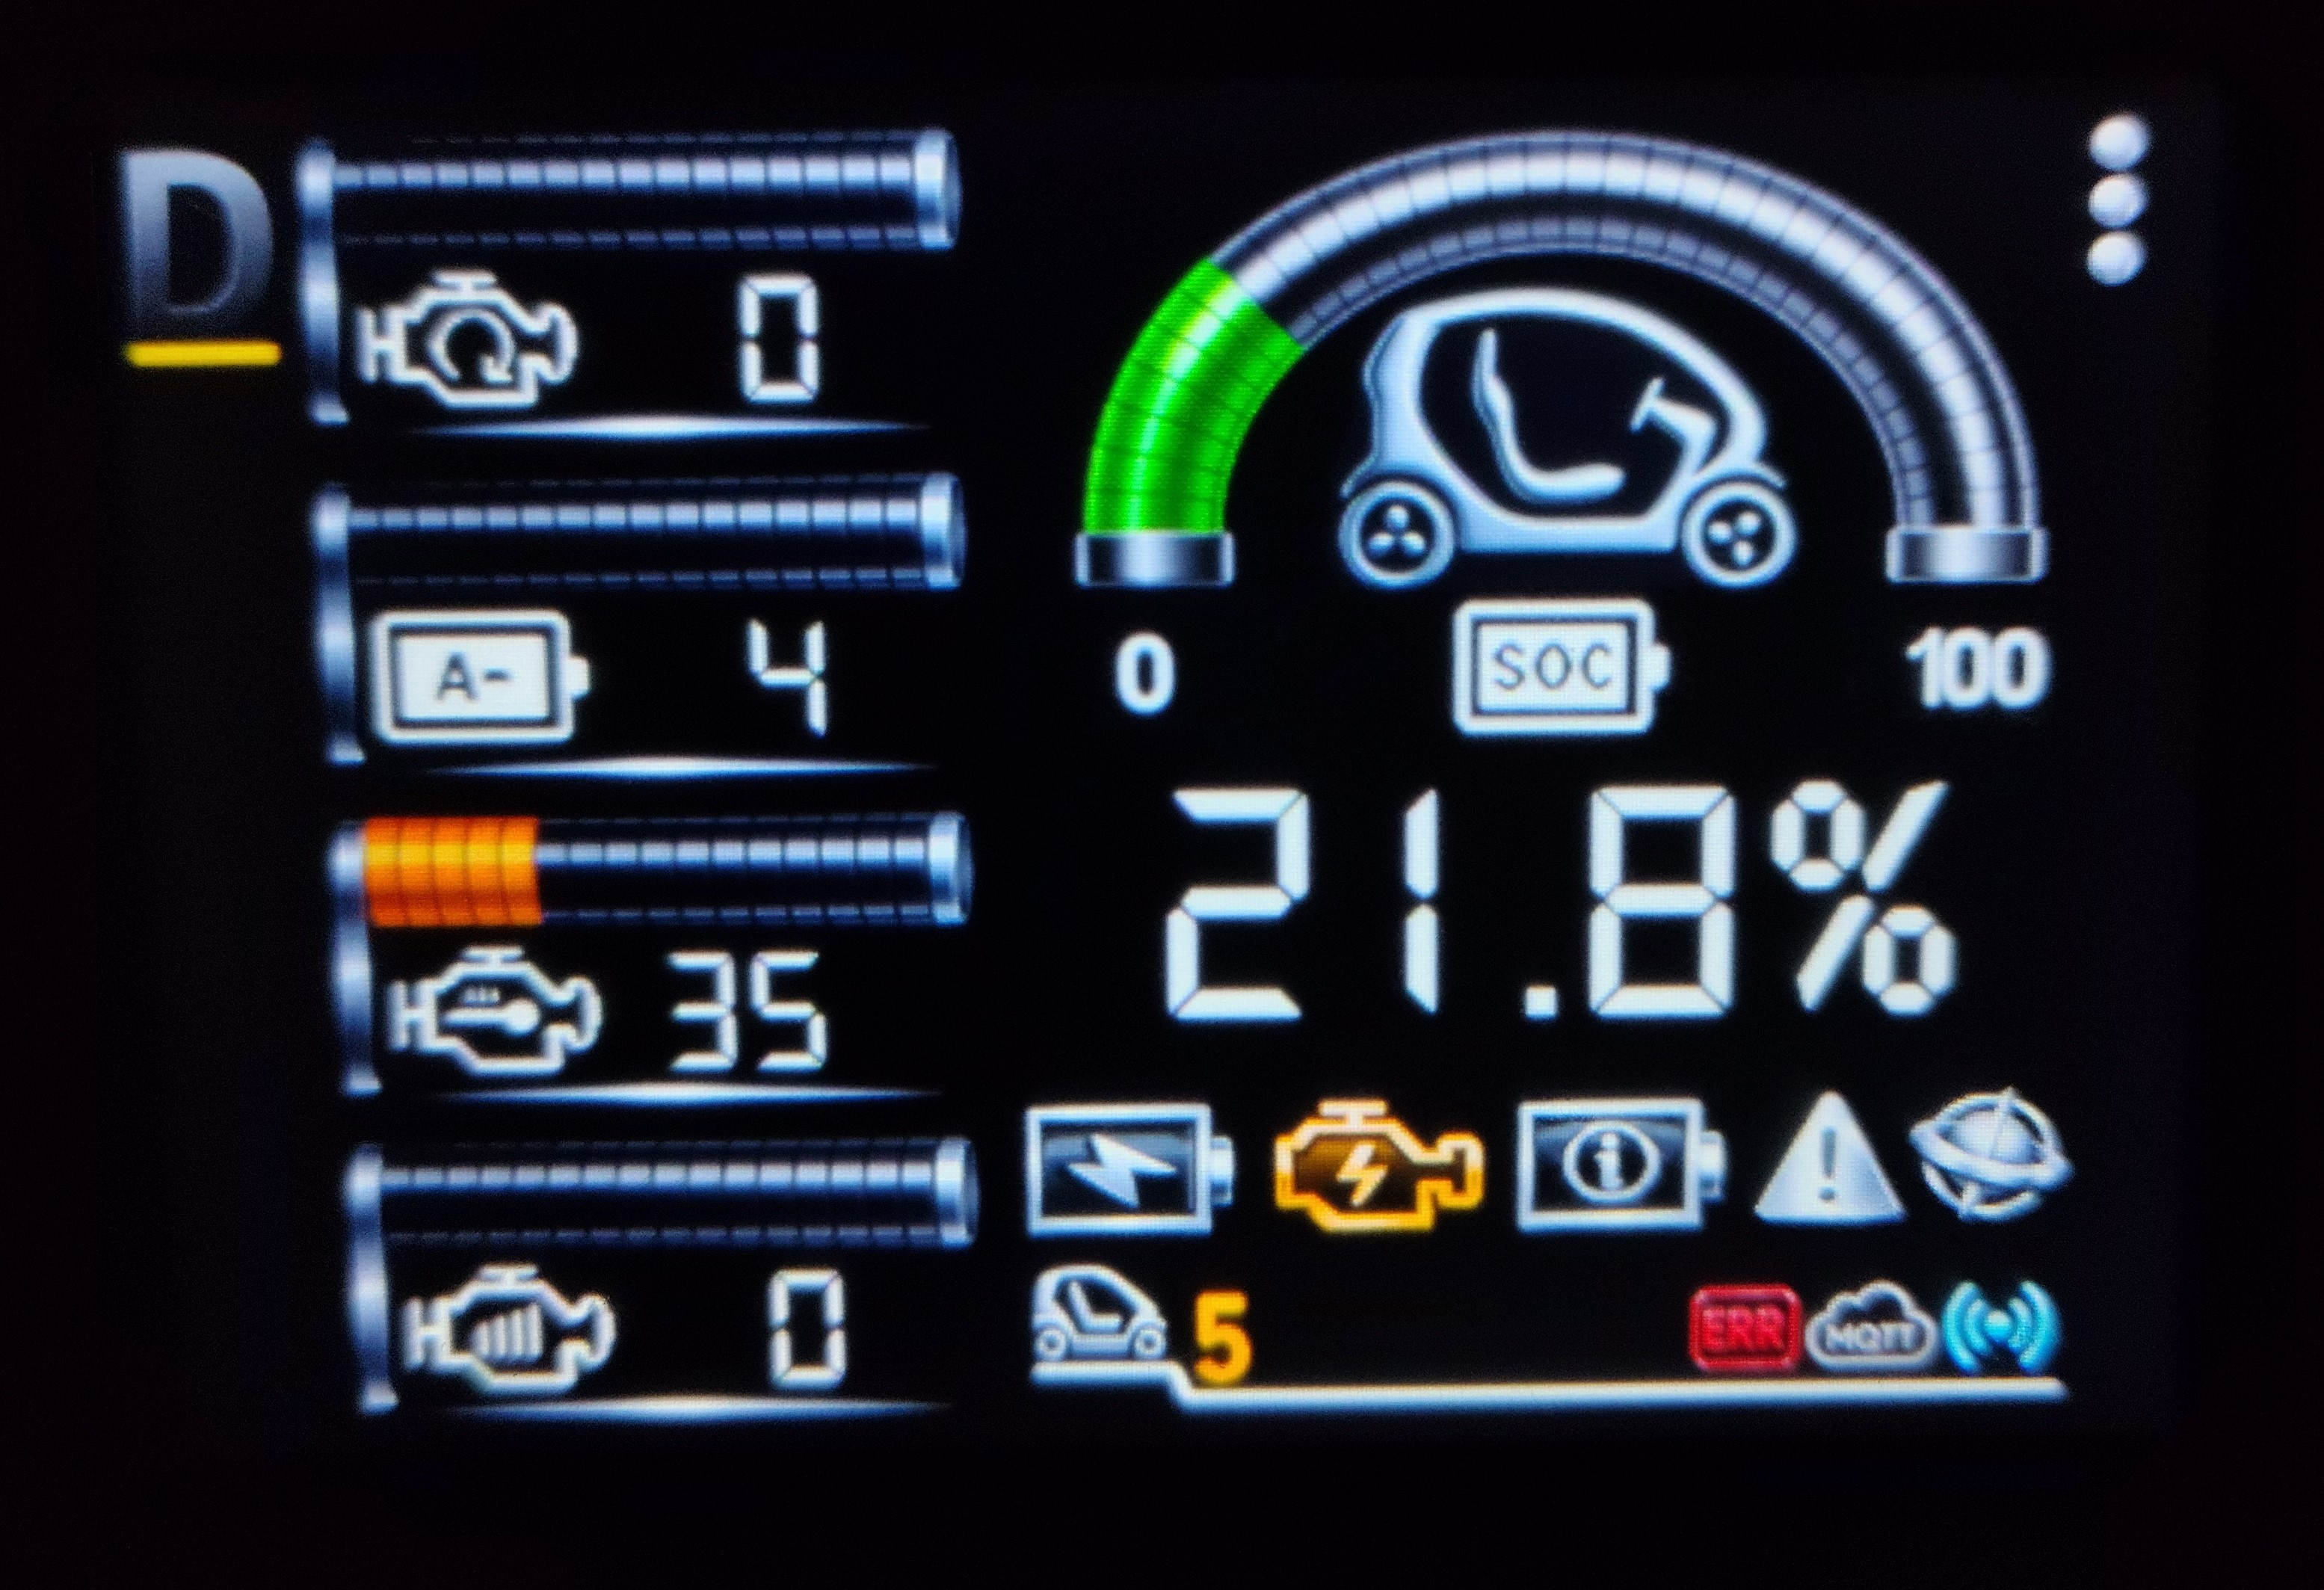
\includegraphics[width=0.8\textwidth]{figures/engine_page.jpg}
    \caption{Beispiel für das gemeinsame Layout (die Motorseite).}
\end{figure}

Auf der linken Seite des Bildschirms befindet sich, wie Sie auf dem Foto sehen können, eine Liste von vier Werten, die in einem minimalen Raster gruppiert sind. Jeder Wert ist mit seiner Maßeinheit und einem kleinen Symbol gekoppelt, das für jede Angabe eindeutig ist und alle in Abschnitt~\ref{sec:icon_list} aufgelistet wurden. 
Über dem Wert befindet sich ein orangefarbener Fortschrittsbalken, der darstellt, wie groß (oder klein) der Wert im Vergleich zu seinem Maximal- (oder Minimal-) Wert ist.\\

Der rechte Bereich des Bildschirms wird hauptsächlich von den Vordergrunddaten (oder einfach den ausgewählten Daten) eingenommen. Er verfügt über ein großes Twizy-Symbol, das von einem bogenförmigen Fortschrittsbalken umgeben ist, der dieselbe Funktion erfüllt wie der zuvor besprochene kleinere, mit dem einzigen Unterschied, dass er 32 statt nur 16 Stufen hat. An den Rändern des Fortschrittsbalkens befindet sich der Bereich oder der Multiplikator des in der Mitte der Seite angezeigten Wertes, welcher dem Symbol zugeordnet ist, das direkt darüber angezeigt wird.\\

Unten befindet sich eine Liste von Symbolen, mit denen zwischen den verschiedenen Seiten des ToM+ gewechselt wird. Die Symbole sind für alle Seiten gleich und wurden in Abschnitt~\ref{sec:page_icon_list} aufgelistet.
In der oberen linken Ecke befindet sich ein kleines Symbol, das den aktuellen Gang des Fahrzeugs anzeigt.
Wenn Sie darauf drücken, \textbf{kehren Sie zur Armaturenbrett-Seite zurück}, die wir gerade besprochen haben.
In der oberen rechten Ecke befinden sich drei kleine Punkte, die bei Betätigung die Einstellungsseite öffnen.
Zu guter Letzt befindet sich auf der langen weißen Linie am unteren Rand des Bildschirms die Statusleiste mit einigen Symbolen, die wir später besprechen werden.

\subsection{Ändern der Vordergrunddaten}

Das Ändern der im Vordergrund angezeigten Daten ist sehr einfach und intuitiv. Sie können dies tun, indem Sie einfach auf das Symbol der Daten tippen, die Sie im Vordergrund anzeigen möchten, und die Werte werden getauscht.
Auf diese Weise können Sie auch die Daten auf der linken Seite des Bildschirms neu anordnen, was sehr nützlich ist, wenn Sie bestimmte Daten in einer beliebigen Reihenfolge haben möchten.

\begin{figure}[H]
    \centering
    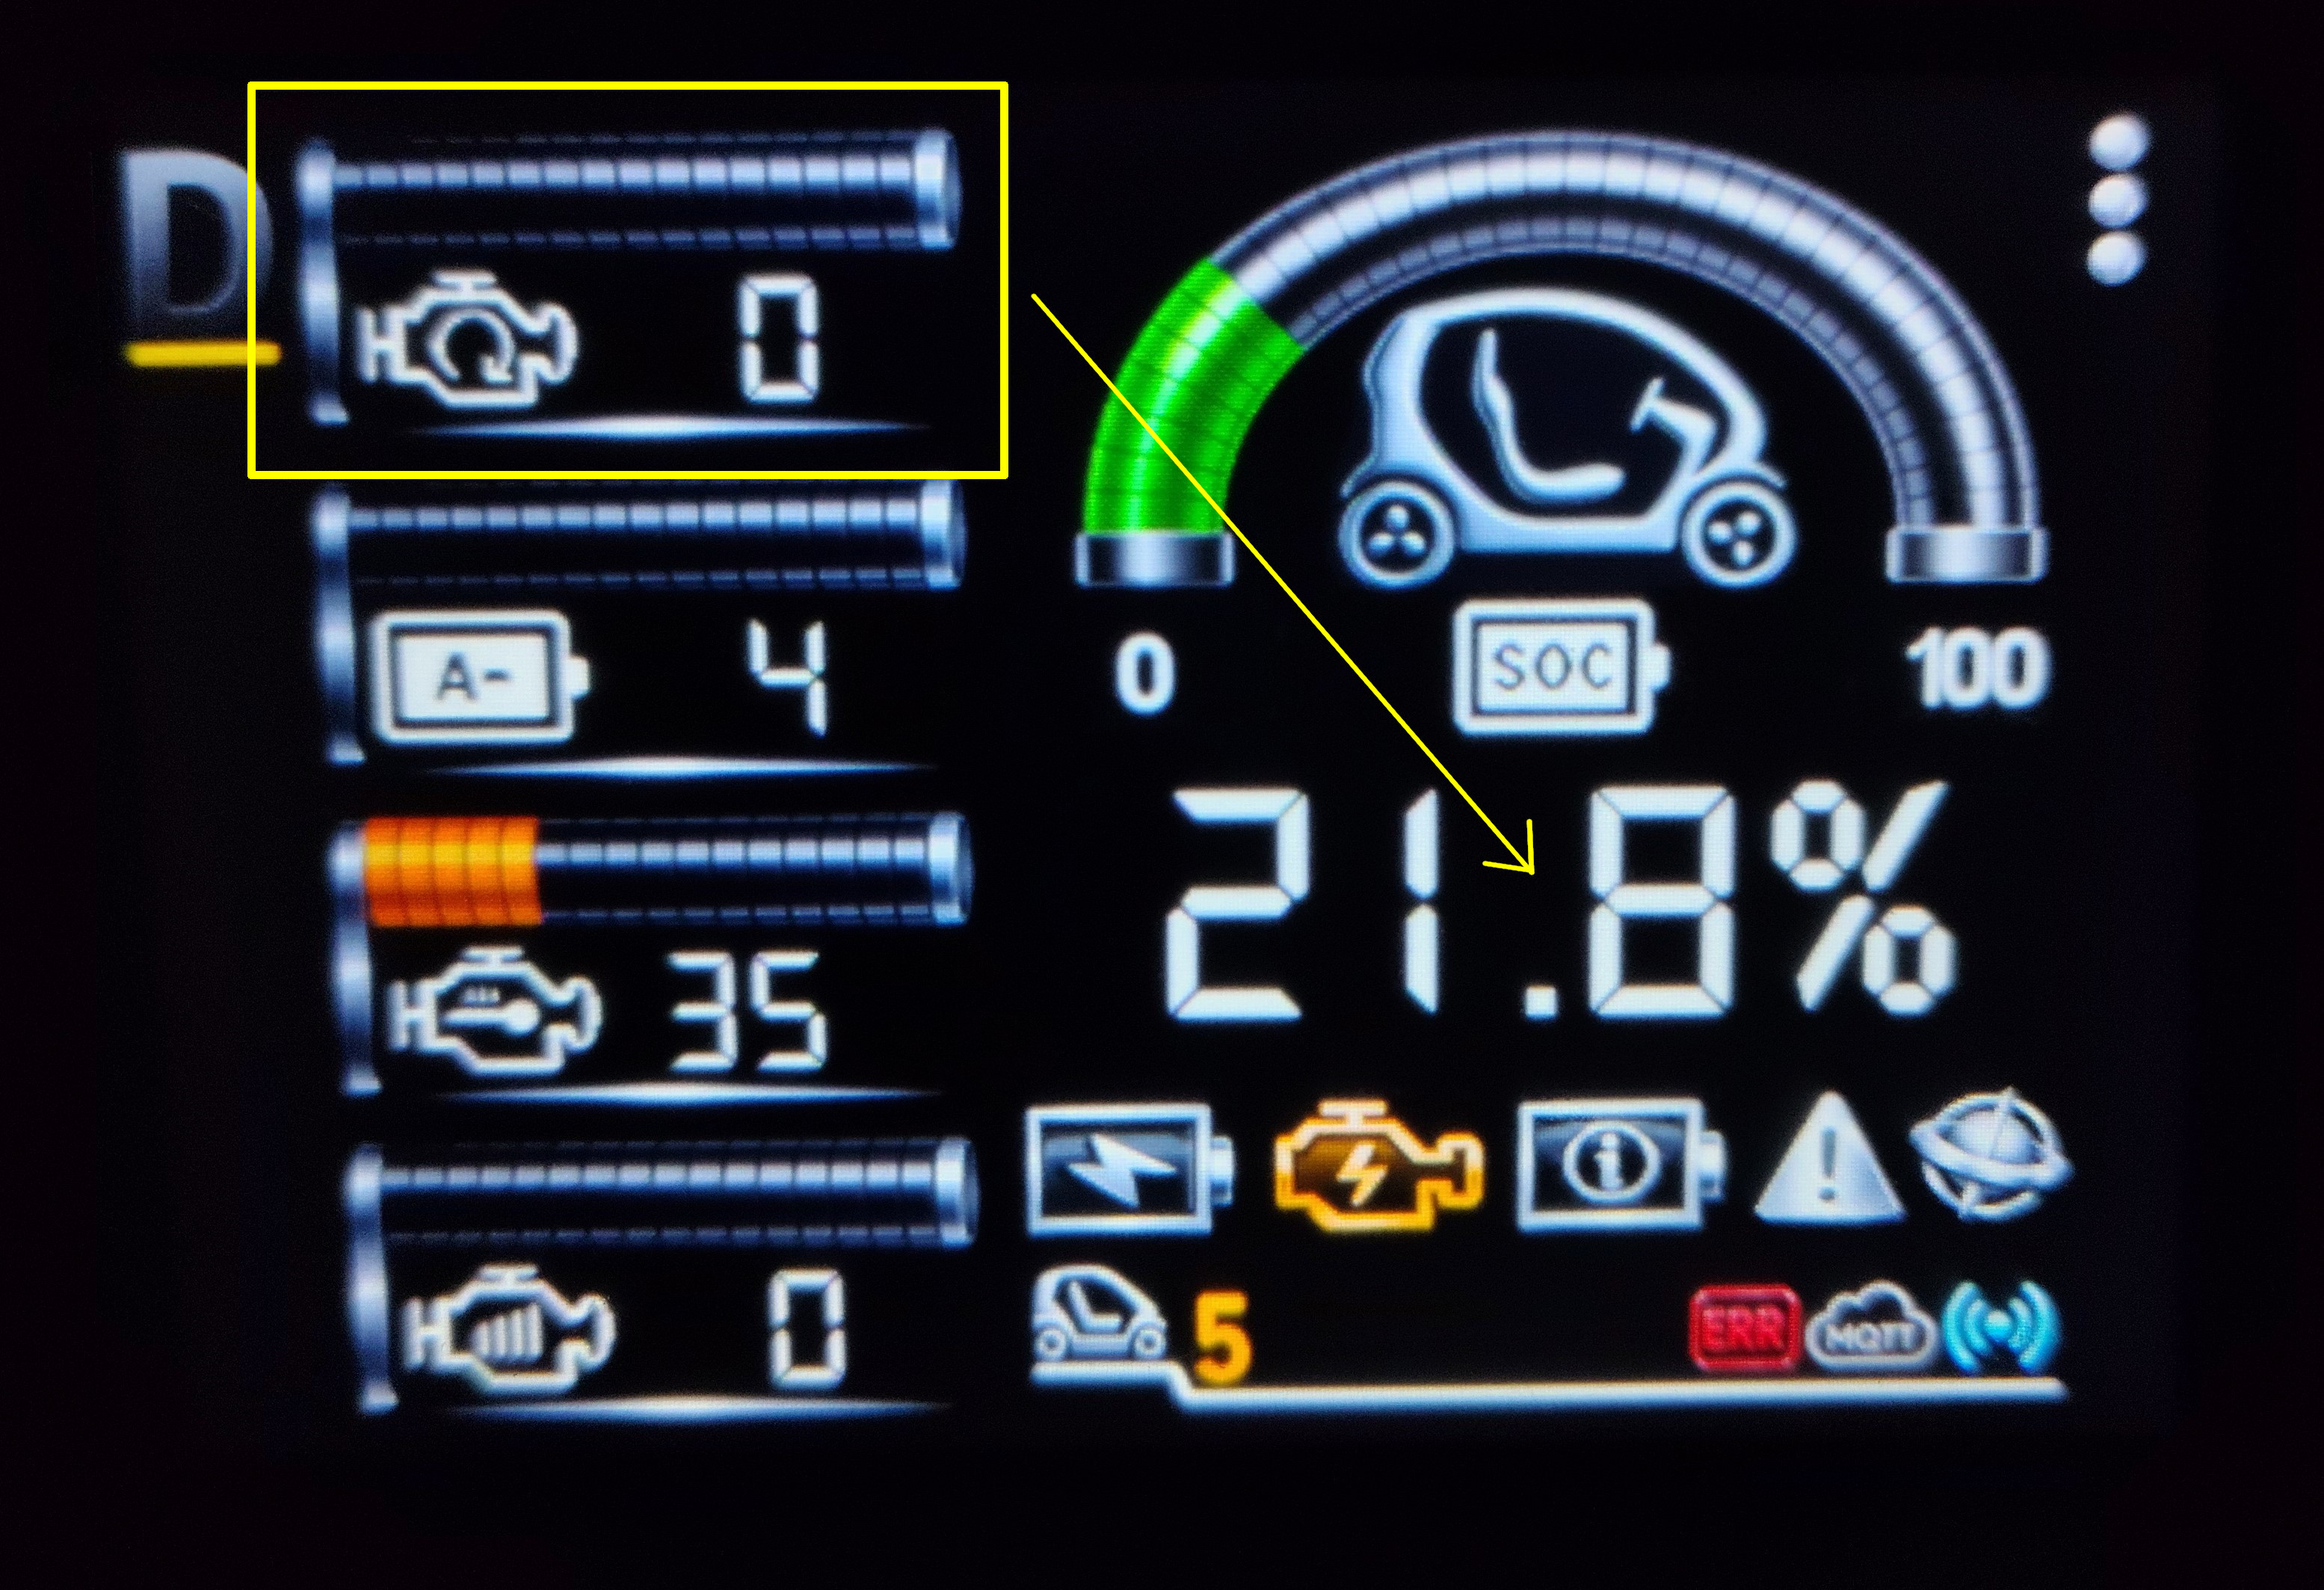
\includegraphics[width=0.7\textwidth]{figures/change_foreground.jpg}
    \caption{Beispiel für das Ändern der Vordergrunddaten (auf der Motorseite).}
\end{figure}

Als Beispiel hat der Benutzer im obigen Bild auf das Symbol der Motordrehzahl getippt, das derzeit auf der linken Seite des Bildschirms angezeigt wird. Die beiden Werte wurden getauscht und nun wird die Motordrehzahl im Vordergrund angezeigt, während der Batterie-SOC im linken Raster angezeigt wird.

\subsection{Ändern der aktiven Seite}

Um die aktive Seite zu ändern, können Sie auf das Symbol der Seite tippen, zu der Sie wechseln möchten. Dieses befindet sich in der unteren Zeile des Bildschirms. Das Symbol wird orange und die neue Seite wird angezeigt.
Im Bild ist die aktive Seite die Motorseite.

\begin{figure}[H]
    \centering
    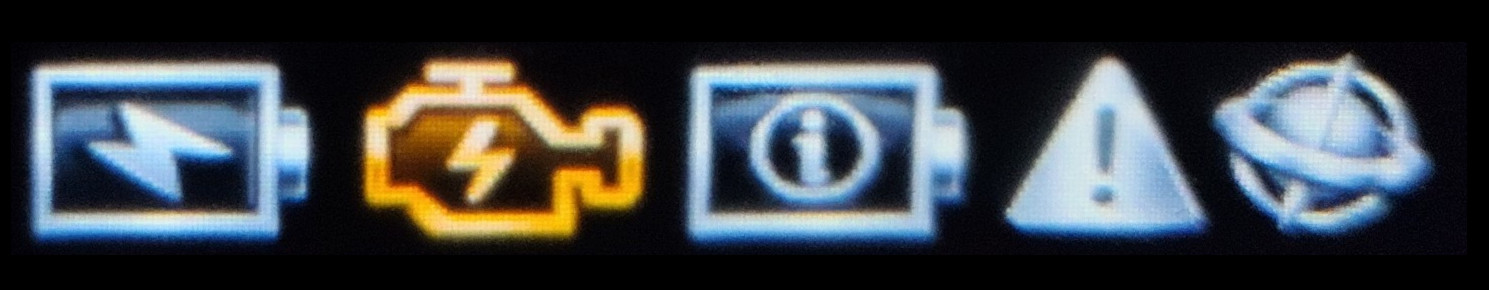
\includegraphics[width=0.7\textwidth]{figures/changing_page.jpg}
    \caption{Beispiel für das Ändern der aktiven Seite (auf der Motorseite).}
\end{figure}

Jede dieser Aktionen kann über die Taste am rechten Scheibenwischerhebel ausgeführt werden, was beim Fahren sehr nützlich ist, da Sie Ihre Augen auf der Straße und Ihre Hände am Lenkrad behalten können. Die Taste kann verwendet werden, um durch die verschiedenen Seiten zu blättern, die Vordergrunddaten zu ändern und vieles mehr. Dies wird im Detail in Abschnitt~\ref{sec:web_wiper_stalk} beschrieben.

\subsection{Die Status-Symbolleiste}
\label{sec:status_icon_bar}

Unterhalb der Tasten zum Seitenwechsel, die im vorherigen Absatz besprochen wurden, befindet sich eine lange weiße Linie, die Ihnen den Status der Netzwerkverbindung anzeigt und auch anzeigt, wann Alarme oder Fehler ausgelöst werden. Am Anfang der Linie befindet sich, wie Sie auf dem Bild sehen können, ein kleines Twizy-Symbol mit einer Nummer: Es ist eine Schaltfläche, die Sie zur Fahrt-Seite führt, die später in Abschnitt~\ref{sec:trip_page} besprochen wird. Schauen wir uns nun die Status-Symbolleiste an.

\begin{figure}[H]
    \centering
    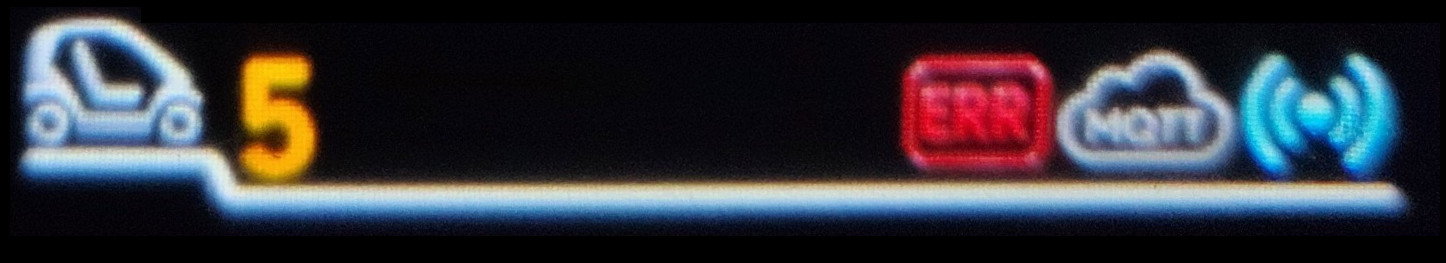
\includegraphics[width=0.7\textwidth]{figures/status_icon_bar.jpg}
    \caption{Die Status-Symbolleiste.}
\end{figure}

Beginnend auf der rechten Seite des Bildes sehen Sie ein magnetisches blaues Wellensymbol, das für den \textbf{Wi-Fi}-Verbindungsstatus steht. Wenn es farbig und fest leuchtet, wie oben gezeigt, bedeutet dies, dass ToM mit einem Wi-Fi verbunden ist, bei dem es sich sowohl um ein öffentliches Netzwerk als auch um eines aus Ihrer festgelegten Liste handeln kann. Wenn das Symbol ausgegraut ist, ist ToM mit keinen Netzwerken verbunden und sucht nach einer Abklingzeit von fünf Minuten erneut nach Wi-Fi-Netzwerken.
Sie können jedoch durch Antippen des Symbols so schnell wie möglich einen neuen Scan erzwingen.
Nicht zuletzt, wenn das Symbol blinkt, hat ToM einen Wi-Fi-Scan durchgeführt, ein oder mehrere Netzwerke gefunden und versucht, sich mit einem von ihnen zu verbinden.\\

Das nächste Symbol ist eine violette Wolke mit dem Text \textbf{„MQTT“} darin und steht, wie Sie erraten können, für den \textbf{MQTT}-Verbindungsstatus. Die Position dieses Symbols ist festgelegt und kann nicht geändert werden, genau wie beim Wi-Fi-Symbol. Eine weitere Ähnlichkeit mit dem vorherigen Symbol besteht darin, dass es entweder fest leuchten oder mit demselben Farbcode wie zuvor ausgegraut sein kann.\\

Dann haben wir das Fehlersymbol, das ein rotes Rechteck mit dem Text \textbf{„ERR“} darin ist.
Es wird angezeigt, wenn ein Fehler vorliegt, oder ausgeblendet, wenn keine Fehler vorhanden sind.\\

Schließlich haben wir Alarmsymbole, die durch farbige Sterne dargestellt werden. Verfügbare Sterne sind die auf dem Bild gezeigten. Sie können auf der Webserver-Seite "Alarmauslöser" auswählen, welchen Sie für jeden Alarm verwenden möchten.
Dort können Sie auch wählen, ob Sie diese blinken lassen möchten oder nicht.

\begin{figure}[H]
    \centering
    
\includegraphics[width=0.7\textwidth]{figures/alarm_icons.png}
    \caption{Die Alarmsymbole.}
    \label{fig:alarm_icons}
\end{figure}

\subsection{Pop-ups}

Auf diesen Seiten werden je nach den auf der Webserver-Seite „Alarmauslöser“ festgelegten Konfigurationen Pop-ups angezeigt. Es gibt zwei Haupttypen von Pop-ups: der erste verschwindet erst, wenn Sie ihn bemerken und darauf drücken (dieser Typ blockiert das gesamte System und pausiert sowohl die Werte im linken Raster als auch den Vordergrundwert). 
Andererseits können Sie, wenn Sie beim Fahren nicht gestört werden möchten, den zweiten Pop-up-Typ verwenden, der speziell dafür entwickelt wurde, nach 10 Sekunden automatisch zu verschwinden. \\

Hier sehen Sie ein Beispiel für die einfachste Art von Pop-up, bei dem das eingekreiste Warnsymbol kontinuierlich blinkt. Wie Sie sehen können, besteht es aus einem gelben Kasten mit einer gepunkteten Umrandung, der das Symbol des Werts und den Wert selbst enthält, der den zuvor auf der Webserver-Seite eingestellten Alarm ausgelöst hat (Motortemperatur = 35\textdegree~C).

\begin{figure}[H]
    \centering
    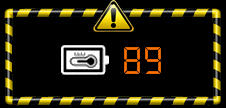
\includegraphics[width=0.7\textwidth]{figures/pop-up.PNG}
    \caption{Ein Beispiel für ein Pop-up.}
\end{figure}


\section{Die Batterie-Info-Seite}

Die Batterie-Info-Seite bietet Ihnen detailliertere Informationen zu jeder einzelnen Zelle der Batterie. Wie Sie vielleicht wissen, haben Standard-Twizy-Batterien 14 Zellen und einen gemeinsamen Temperatursensor für jedes Paar.
Auf dieser Seite können Sie die Spannung und Temperatur jeder Zelle überwachen und haben auch einen Überblick über die Gesamtspannung der Batterie. Auf dem Bild ist zu sehen, wie dies normalerweise aussieht.

\begin{figure}[H]
    \centering
    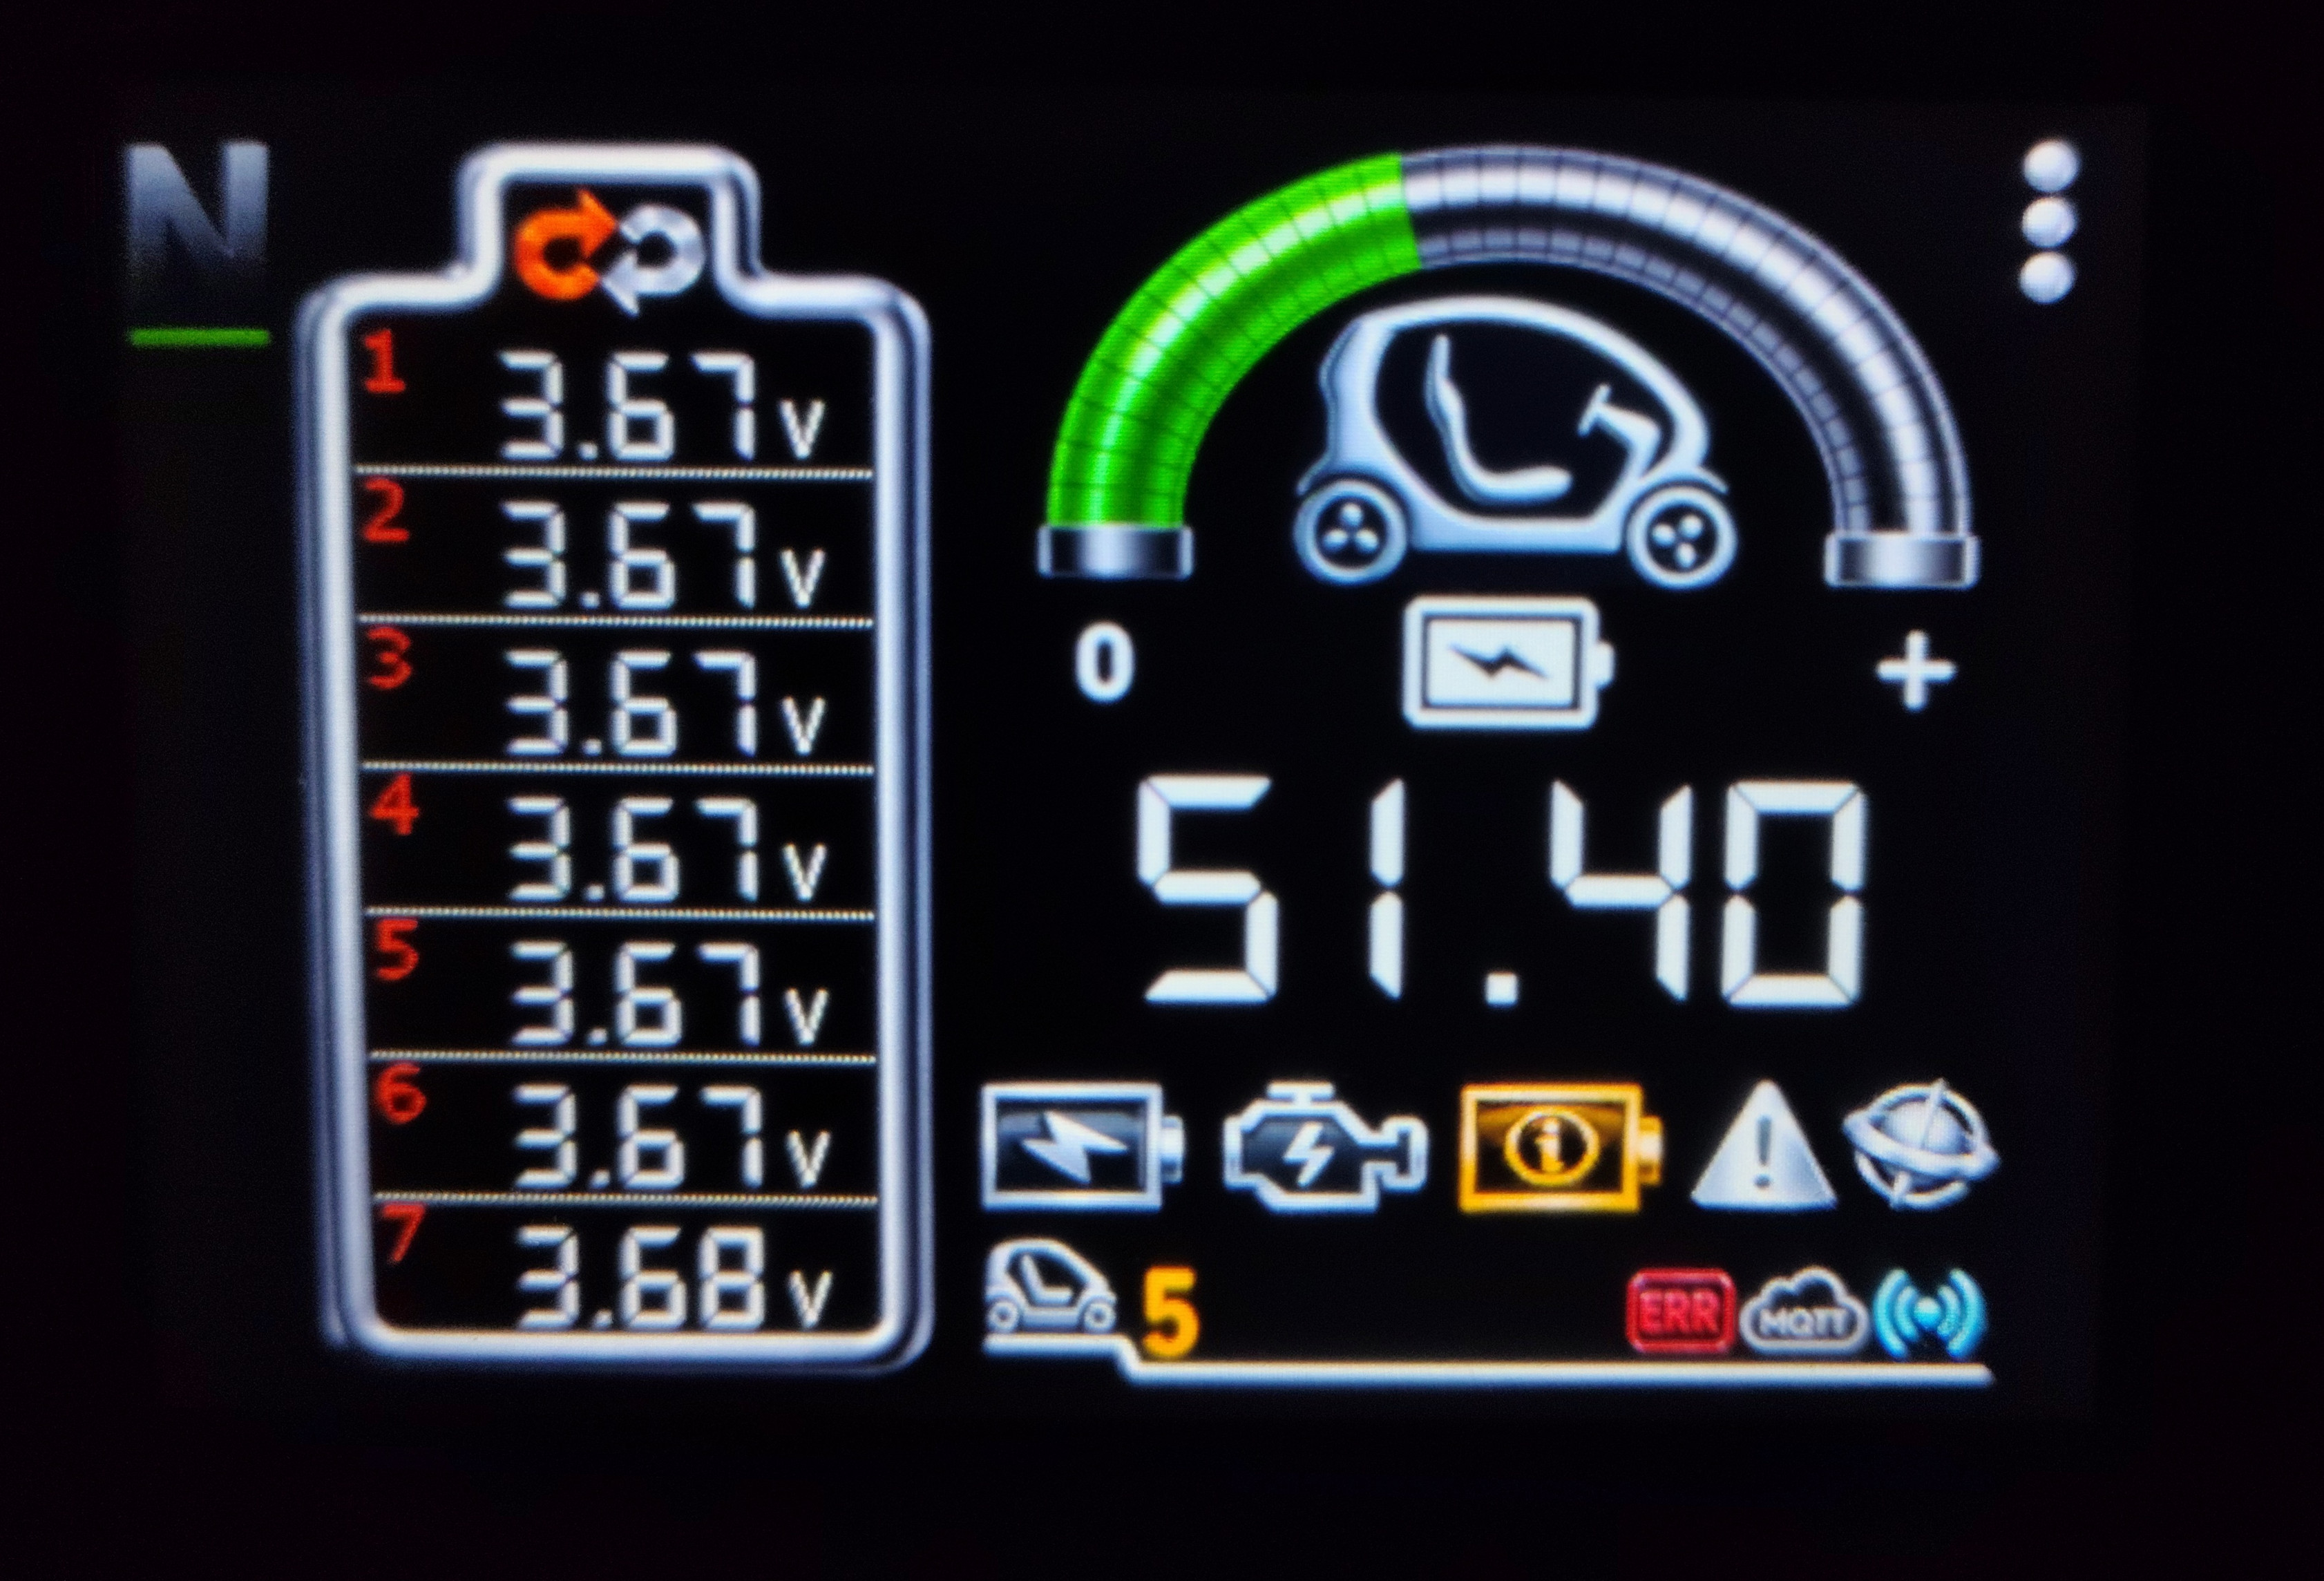
\includegraphics[width=0.8\textwidth]{figures/binfo_page.jpg}
    \caption{Die Batterie-Info-Seite.}
\end{figure}

\subsection{Überprüfen von Spannung und Temperatur}

Wie auf dem Bild oben auf der linken Seite der Seite gezeigt, befindet sich eine batterieförmige weiße Linie, die eine kleine Tabelle mit den Spannungen der ersten sieben Zellen enthält. Um die restlichen Zellenspannungen zu sehen, drücken Sie das orange und weiße Pfeilsymbol (das auf dem nächsten Foto eingekreist ist) und das Raster zeigt die nächsten Werte an.


Wenn Sie dieselbe Pfeiltaste erneut drücken, ändern sich die angezeigten Daten erneut und es werden die Zelltemperaturen in Celsius ausgedrückt. Der Vordergrundwert würde sich ebenfalls ändern und wie Sie an dem Symbol darüber erkennen können, wird die Gesamttemperatur der Batterie angezeigt, die in diesem Beispiel für jede Zelle gleich ist. Beziehen Sie sich auf das Bild unten, um die Änderung zu sehen.

\begin{figure}[ht]
    \centering

    \begin{subfigure}[t]{0.48\textwidth}
        \centering
        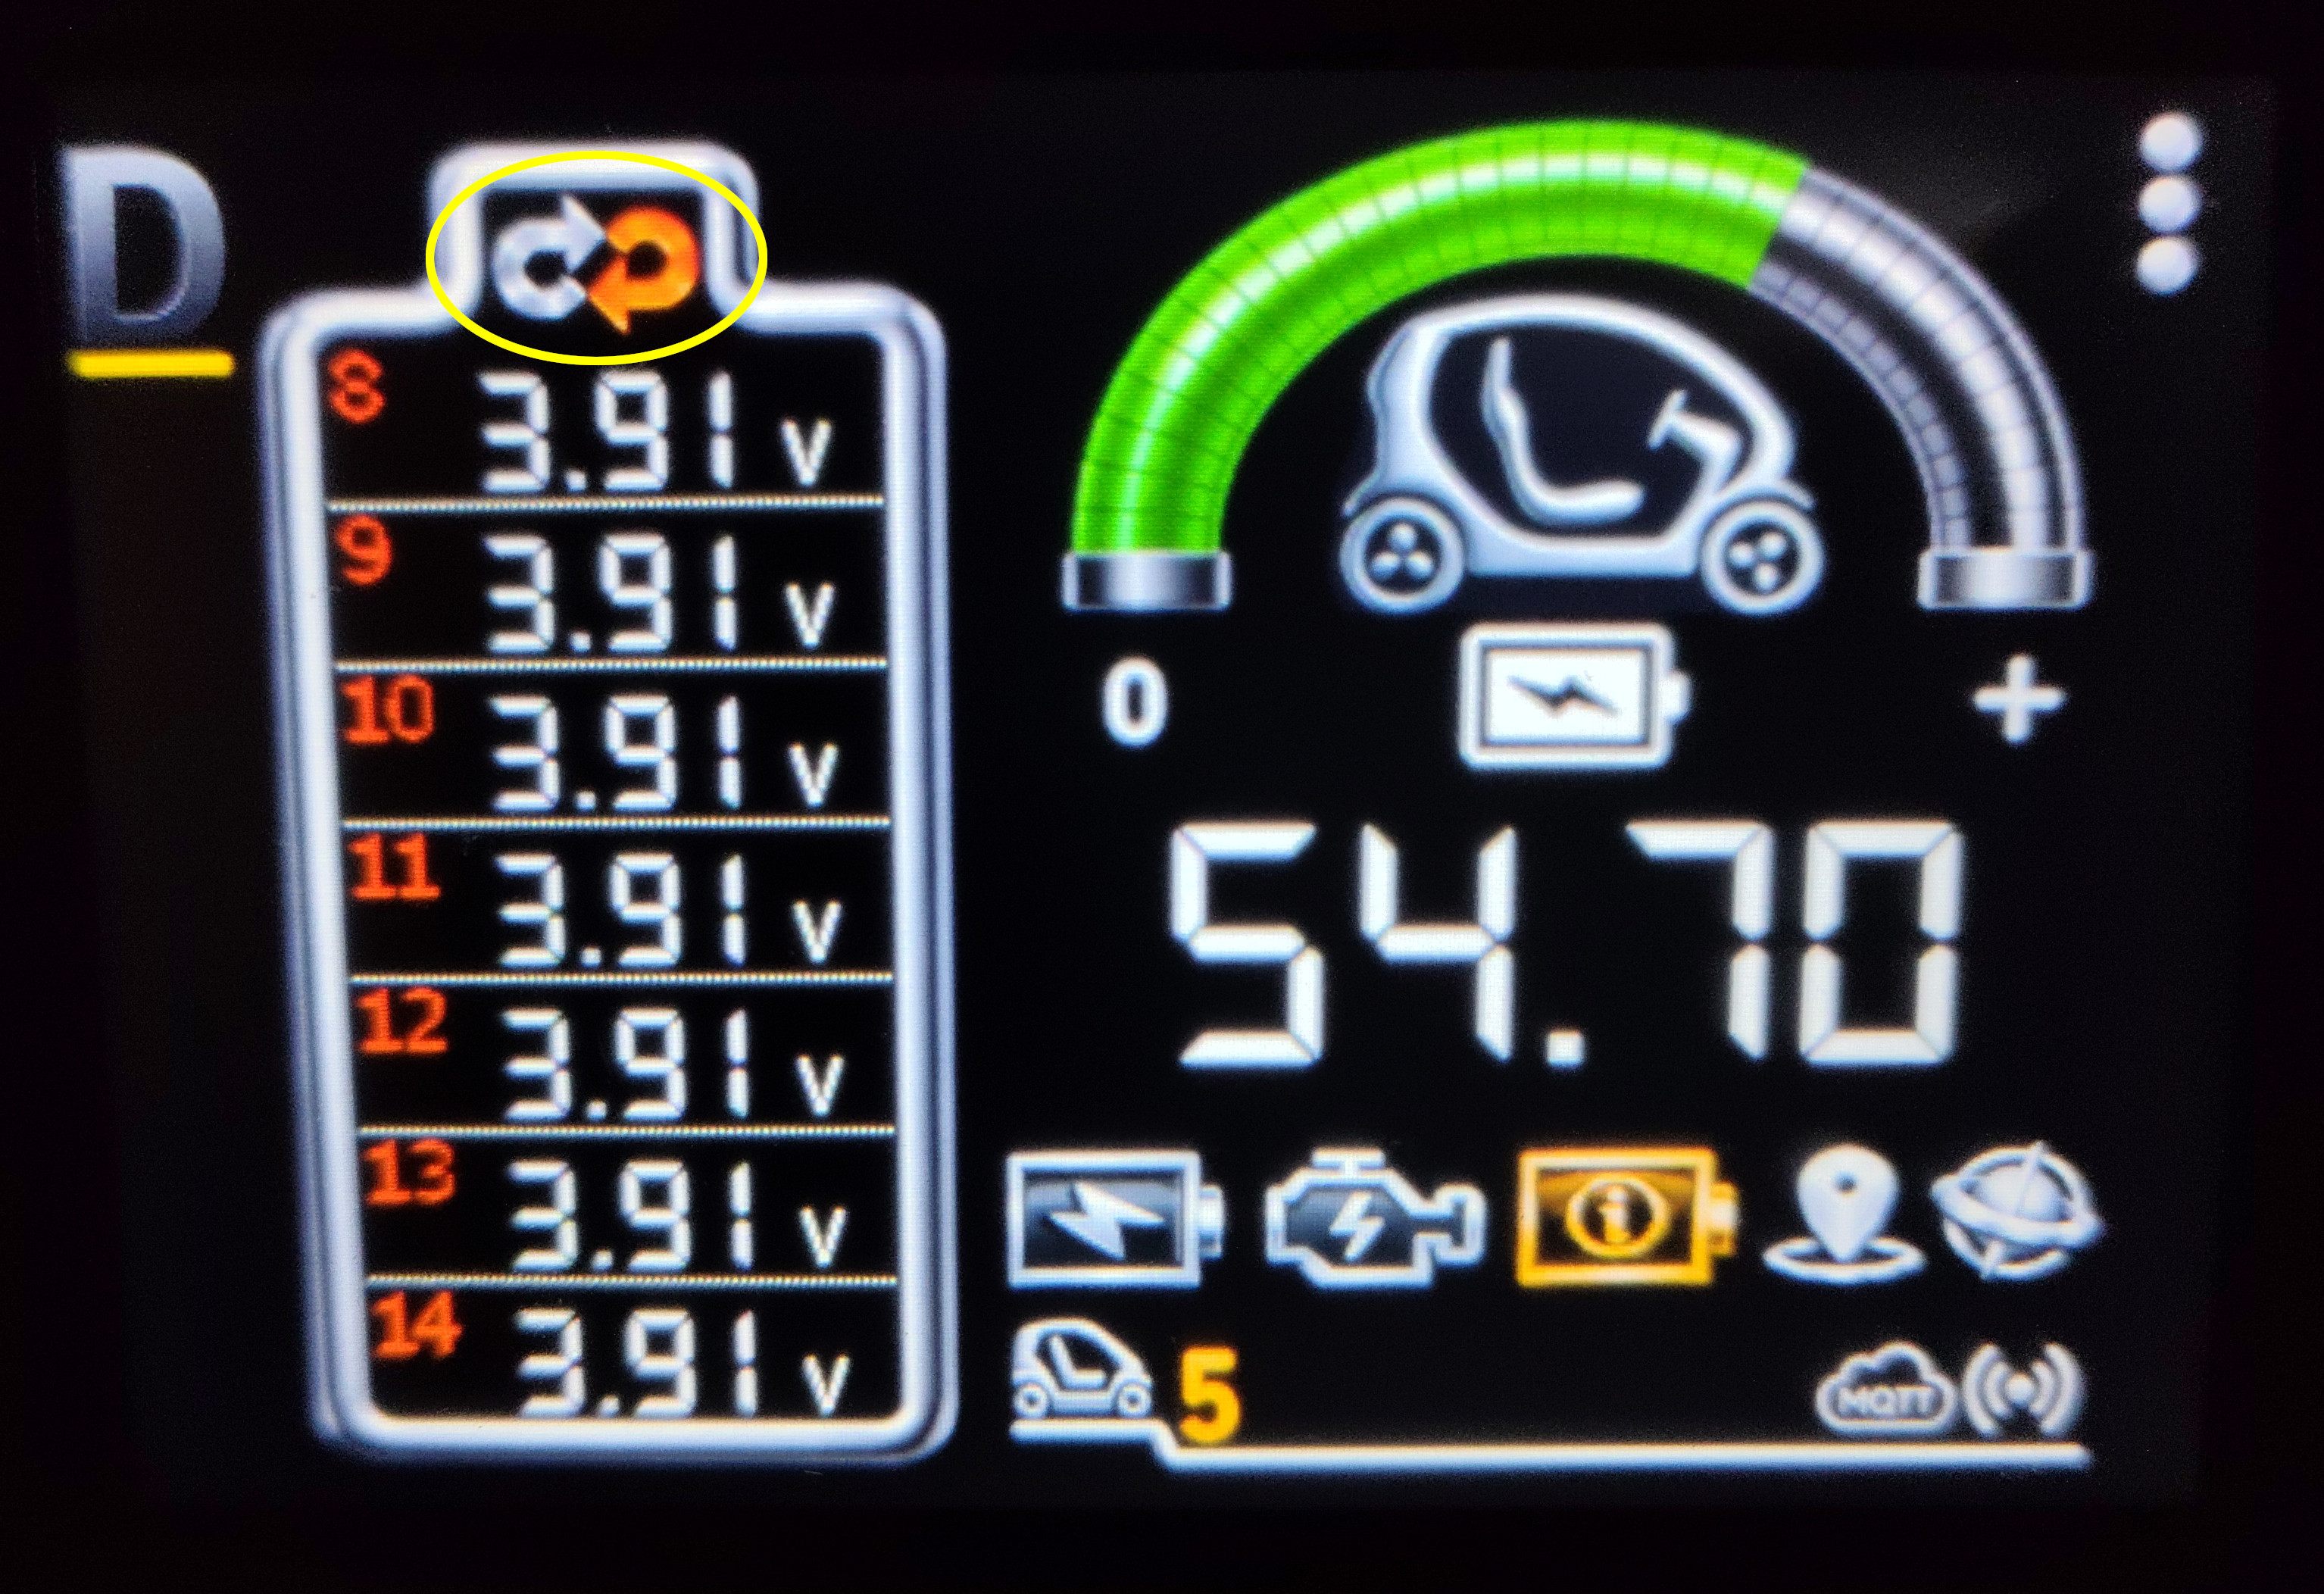
\includegraphics[width=\linewidth]{figures/binfo_page2.jpg}
        \caption{Verbleibende Zellspannungen.}
    \end{subfigure}
    \hfill
    \begin{subfigure}[t]{0.48\textwidth}
        \centering
        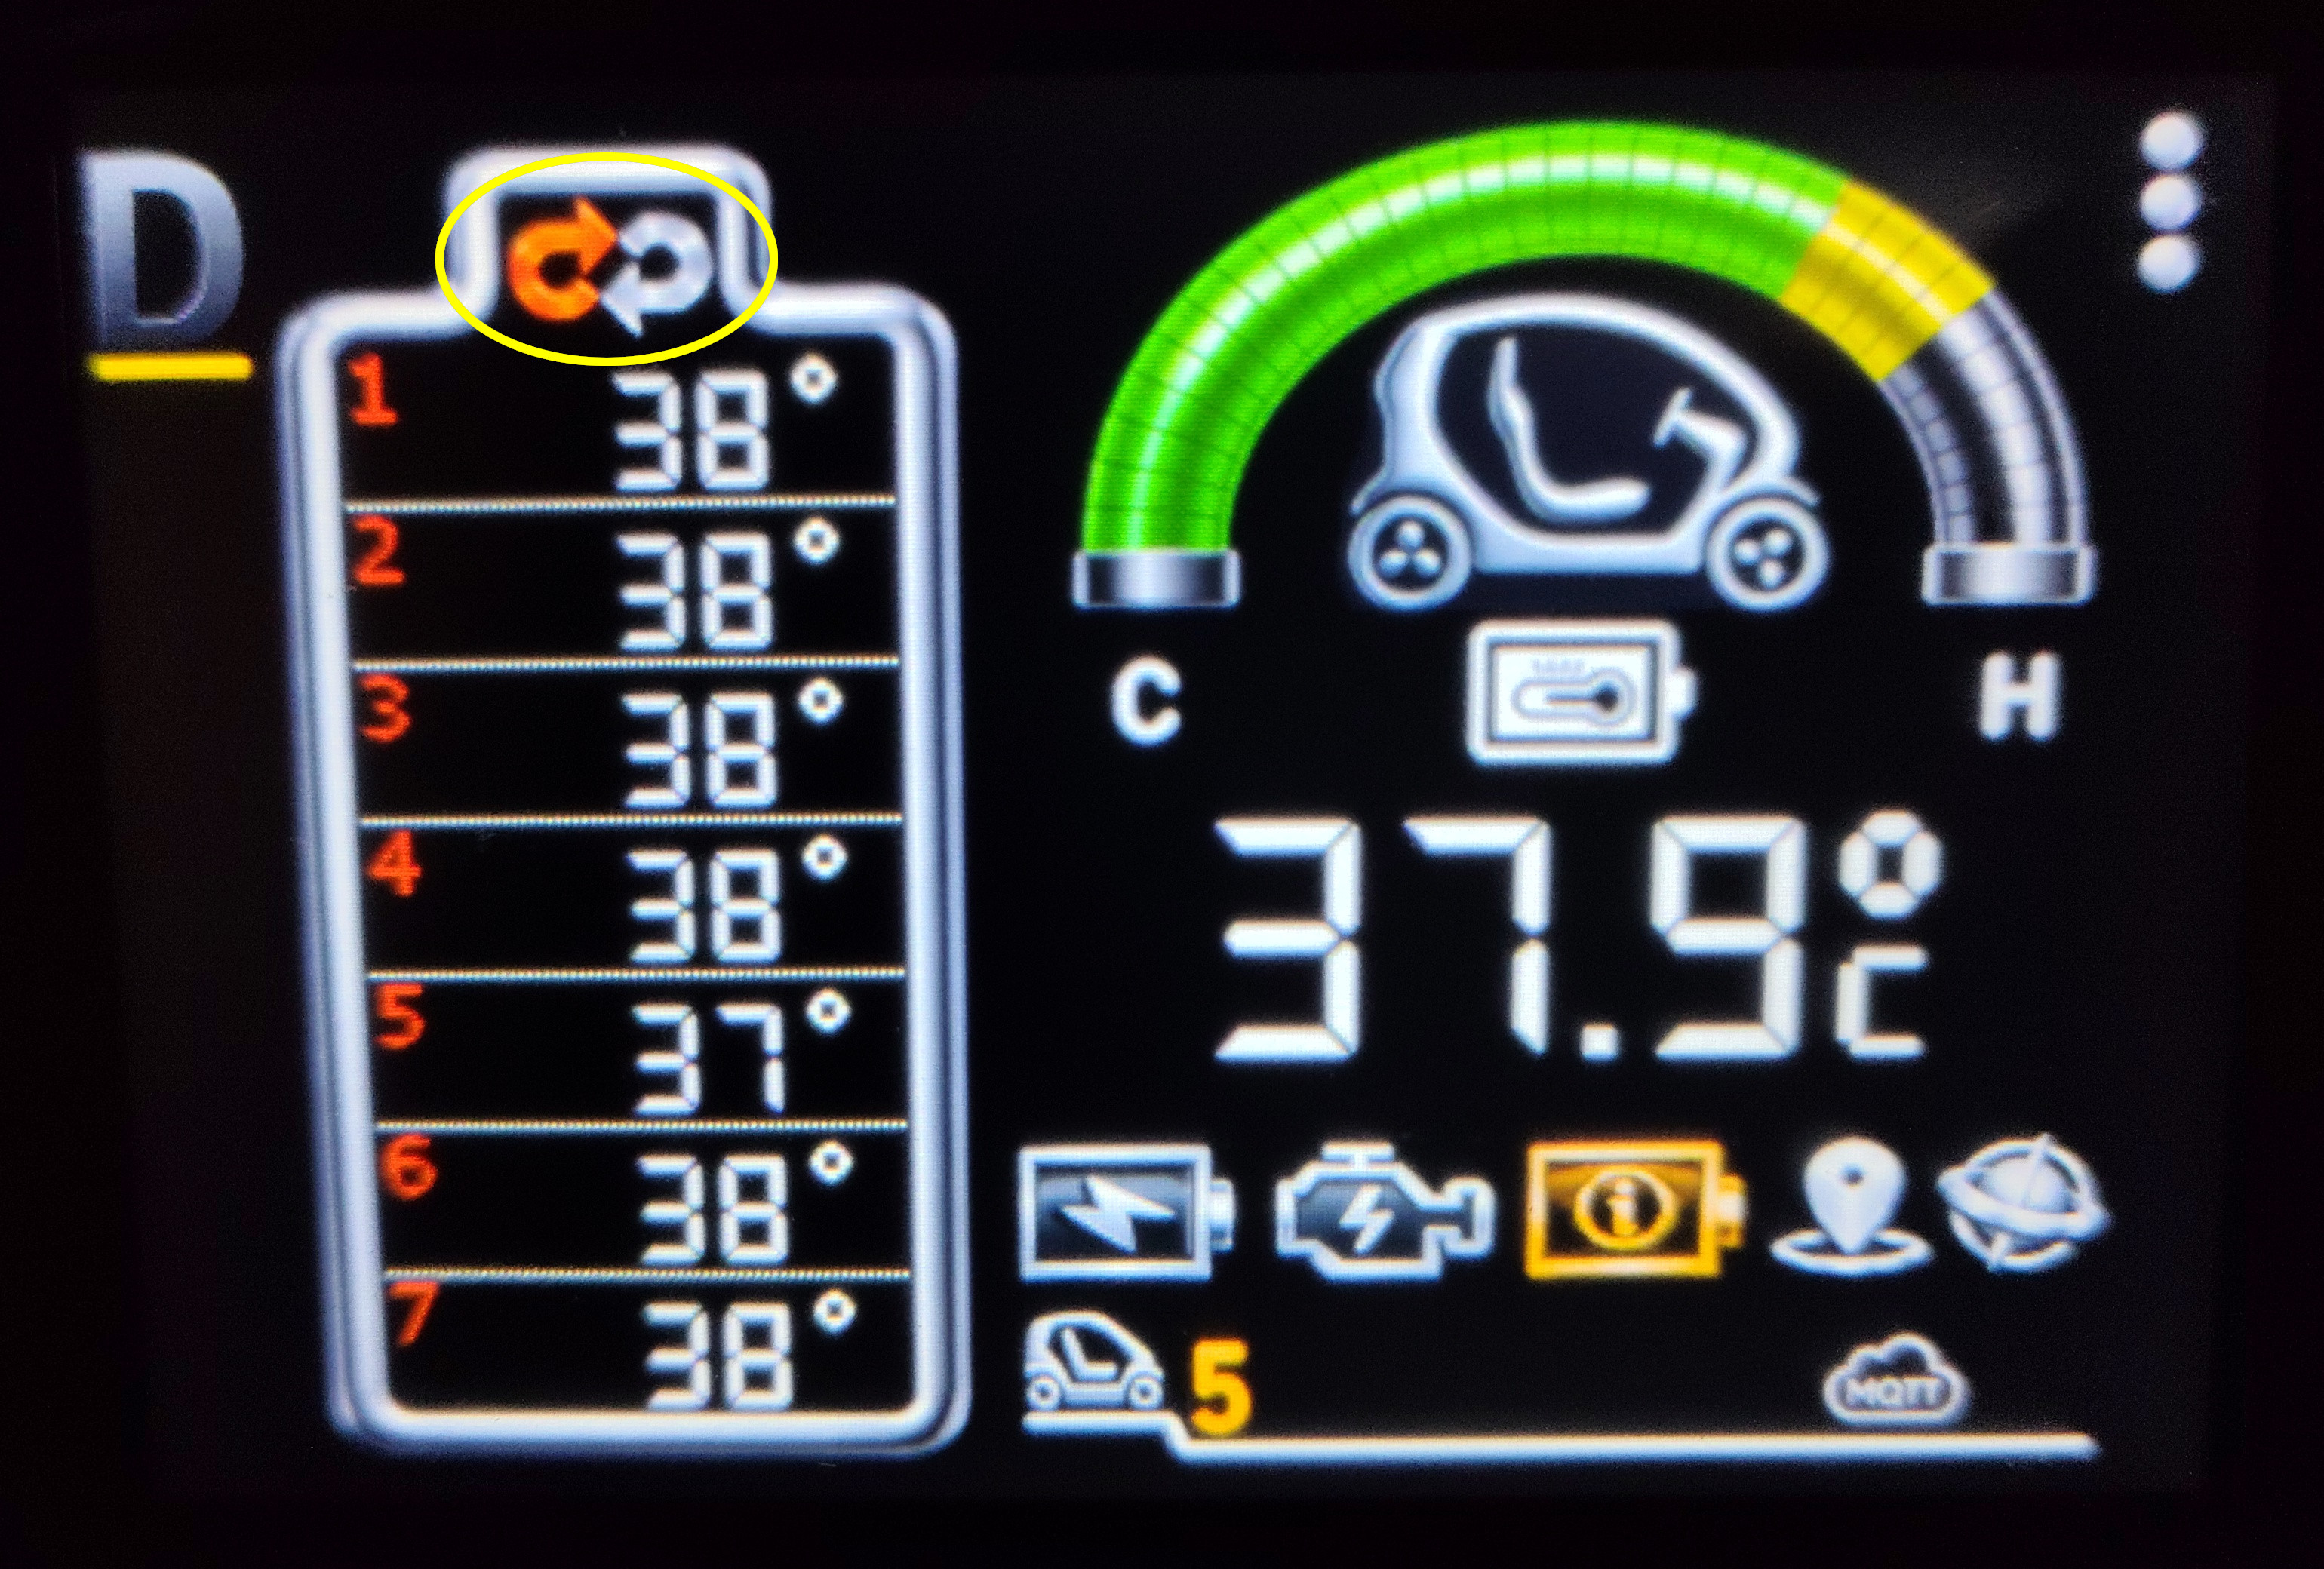
\includegraphics[width=\linewidth]{figures/binfo_page3.jpg}
        \caption{Zelltemperaturen.}
    \end{subfigure}
\end{figure}

\subsection{Die komprimierte Batterie-Info-Seite}
\label{sec:condensed_binfo}

Ein erneutes Drücken derselben Taste führt Sie zu einer speziellen Seite, die alle Daten, die wir im vorherigen Absatz besprochen haben, auf einmal enthält.

\begin{figure}[H]
    \centering
    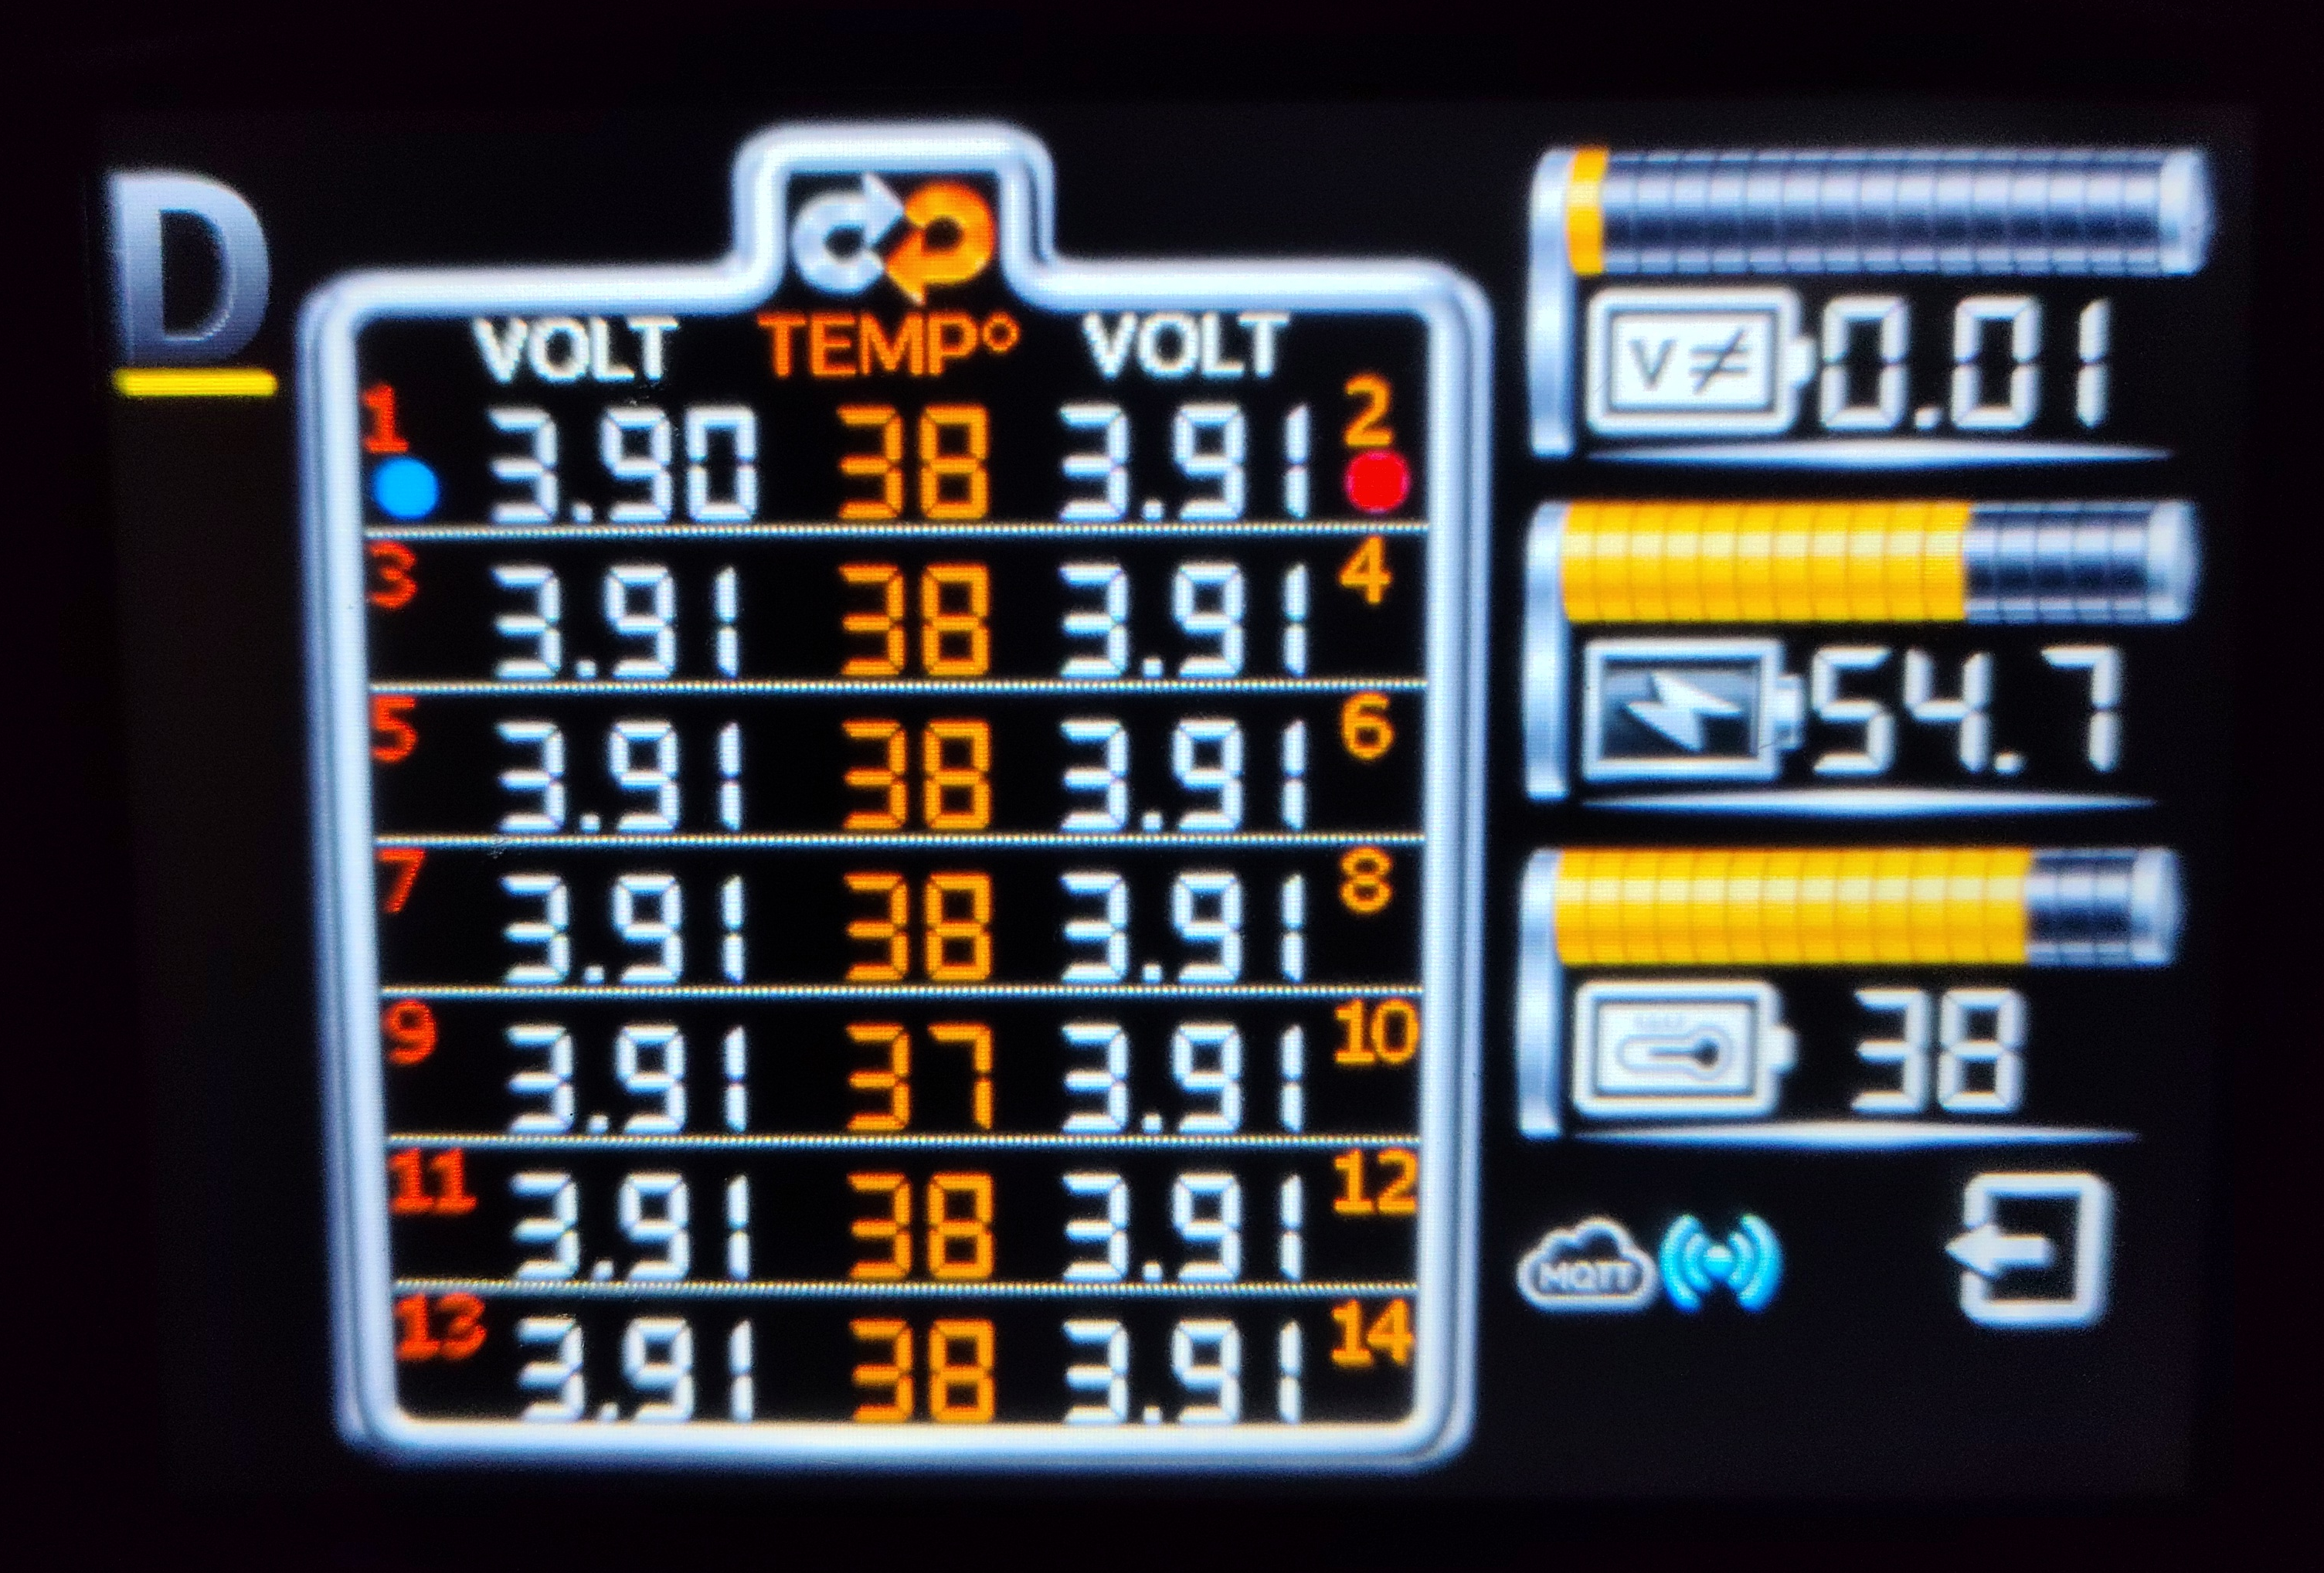
\includegraphics[width=0.8\textwidth]{figures/binfo_page_condensed.png}
    \caption{Die komprimierte Batterie-Info-Seite.}
\end{figure}

Auf dem Foto oben sehen Sie, dass der Bildschirm in zwei Teile geteilt ist. Der erste ist die gleiche batterieförmige weiße Linie, aber etwas größer, um alle Spannungs- und Temperaturwerte aufzunehmen. Die Temperatur befindet sich zwischen den beiden Zellen, die diesen Temperatursensor gemeinsam nutzen. Auf der rechten Seite der Seite sehen Sie den Wert, der zuvor im Vordergrund angezeigt wurde, d. h. die Gesamtspannung der Batterie und die Gesamttemperatur der Batterie. Der SOC-Wert steht ebenfalls an erster Position, da er immer nützlich ist.\\

Auf dieser Seite gab es nicht genug Platz für die Schaltflächen zum Seitenwechsel, da es wichtiger ist, die zuvor besprochenen Status-Symbole zu haben. Wenn Sie die Seite wechseln müssen, können Sie die Beenden-Schaltfläche in der unteren rechten Ecke drücken und gelangen dann auf eine Seite, die über die Steuerelemente zum Ändern der aktiven Seite verfügt.\\

Ein wichtiger Hinweis des letzten Updates ist der Unterschied zwischen der Zelle mit der minimalen und der maximalen Spannung, die durch einen blauen bzw. roten Punkt dargestellt werden. Dieser Wert ist sehr wichtig, da er Ihnen sagen kann, ob die Batterie gesund ist oder nicht. Wenn der Unterschied zu hoch ist, bedeutet dies, dass die Batterie unausgeglichen ist und dies ein Zeichen für ein Problem sein könnte. ToM+ zeigt Ihnen diesen Wert auf der komprimierten Batterie-Info-Seite an, und Sie können auch im Webserver einen Alarmauslöser einstellen, um benachrichtigt zu werden, wenn der Unterschied zu hoch ist.\\

Sie können in den Einstellungen festlegen, ob diese komprimierte Batterieseite als Standardseite angezeigt wird, wenn Sie auf die Schaltfläche Batterie-Info drücken, oder nicht. Der Vorgang wird in Abschnitt~\ref{sec:settings_page} gezeigt. Wenn Sie die Option wählen, alle vier in diesem Absatz behandelten Seiten anzuzeigen, können Sie auch die Pfeiltaste drücken, während Sie sich auf der komprimierten Seite befinden, um zurück zu den anderen Batterie-Info-Seiten zu blättern.

\section{Die Alarmprotokoll-Seite}
\label{sec:alarm_log}

Auf dieser Seite können Sie alle Alarmauslöser sehen, falls Sie einen verpasst haben oder wenn Sie diese stummgeschaltet haben, um während der Fahrt nicht gestört zu werden. Schauen wir uns an, wie es aussieht.

\begin{figure}[H]
    \centering
    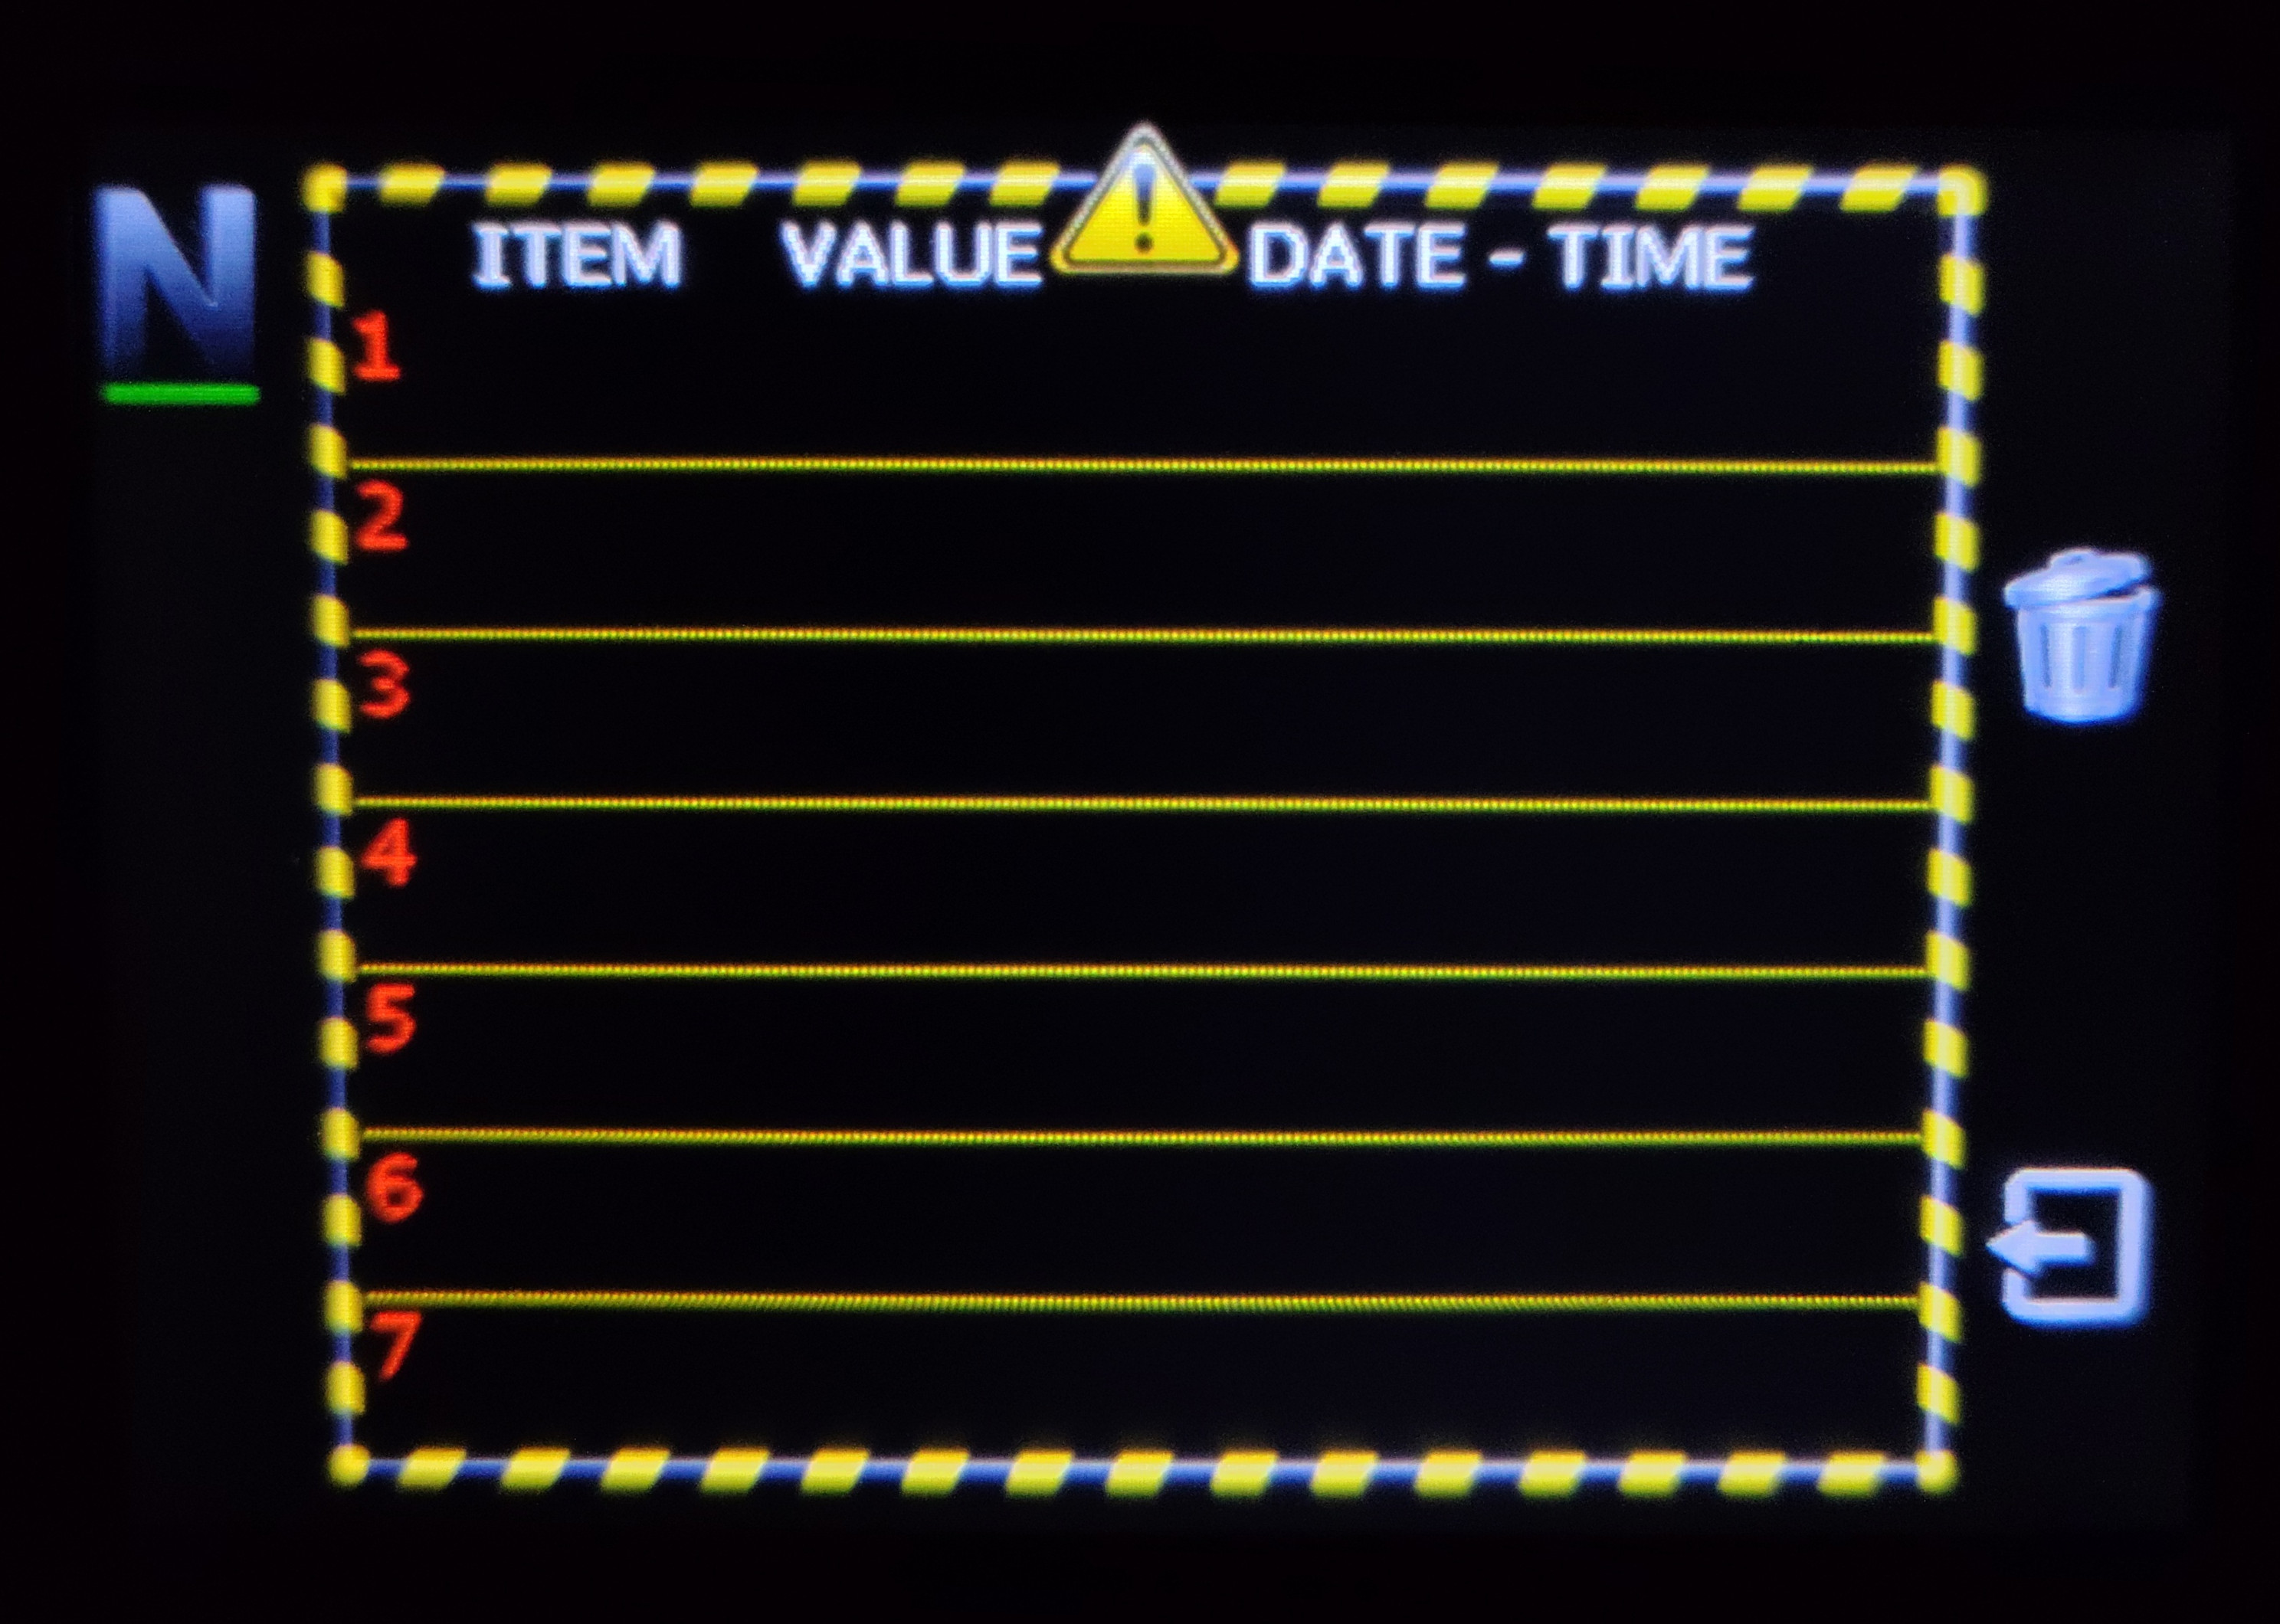
\includegraphics[width=0.8\textwidth]{figures/alarm_page.jpg}
    \caption{Die 3D-Alarmprotokoll-Seite.}
\end{figure}

Das Bild zeigt eine kleine Tabelle, die das Element, das den Alarm ausgelöst hat, gepaart mit seinem Symbol und seinem Wert enthält. Dann habe ich auch noch Datum und Uhrzeit hinzugefügt (verfügbar, wenn beim ersten Mal eine Verbindung zu einem Netzwerk hergestellt wurde), um zu wissen, wann dieser Datensatz der Liste hinzugefügt wurde.\\

In den nächsten Bildern (mit dem alten Design) beziehen sich die meisten Datensätze auf den Batterie-SOC, insbesondere, wenn er unter 30 \% fällt. In Abschnitt~\ref{sec:web_alarm_triggers} erfahren Sie, wie Sie Ihren eigenen Alarm auf dem Webserver einrichten.

\begin{figure}[H]
    \centering
    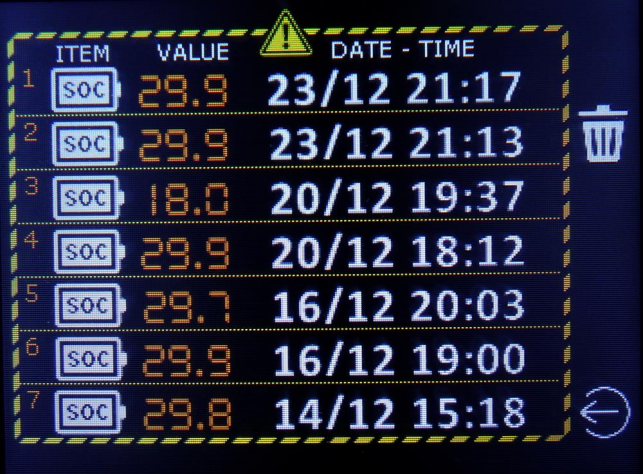
\includegraphics[width=0.7\textwidth]{figures/alarm_log_old1.png}
    \caption{Die 3D-Alarmprotokoll-Seite.}
\end{figure}

\subsection{Überprüfen älterer Alarmauslöser}

Wenn Sie ältere Alarmauslöser sehen müssen, die nicht in der Liste der ersten sieben aufgeführt sind, können Sie das gelbe Warnsymbol oben in der Tabelle drücken. Dadurch ändern sich die angezeigten Werte in die älteren. Sie können diese Aktion zweimal durchführen, da ToM bis zu 21 Alarmauslöser speichern kann und ältere vergisst.

\begin{figure}[H]
    \centering
    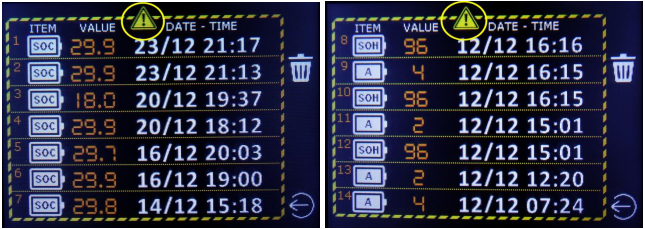
\includegraphics[width=1\textwidth]{figures/alarm_log_old2.png}
    \caption{Ändern der angezeigten Auslöser.}
\end{figure}

Wie Sie auf diesen beiden Fotos der Alarmprotokoll-Seite sehen können, änderten sich die angezeigten Daten beim Drücken der eingekreisten gelben Warnschaltfläche auf einige der älteren, was Sie beim Vergleich der Daten feststellen können. Der Elementzähler links hat sich ebenfalls geändert (8--14).

\subsection{Löschen eines Alarmauslösers}
\label{sec:delete_log_record}

Wenn Sie einen oder mehrere Datensätze nicht mehr benötigen, können Sie auswählen, ob einige davon gelöscht werden sollen. Wählen Sie einen oder mehrere Datensätze zum dauerhaften Entfernen aus, indem Sie auf das Datum oder die Uhrzeit drücken (ein kleines rotes Häkchen erscheint neben den ausgewählten Datensätzen). Drücken Sie dann auf das gelb eingekreiste Mülleimer-Symbol im zweiten Foto, um die ausgewählten Datensätze zu löschen. Diese Datensätze verschwinden und werden durch die nächsten Datensätze ersetzt, was zu einer Verschiebung der gesamten Liste führt, wie Sie auf dem zweiten Bild erkennen können.

\begin{figure}[H]
    \centering
    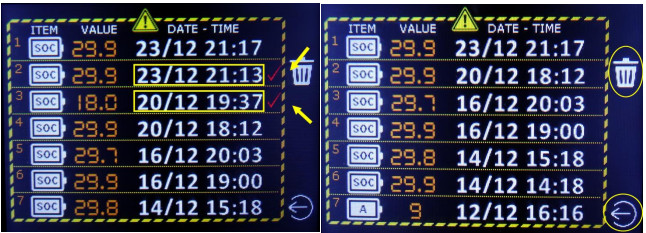
\includegraphics[width=1\textwidth]{figures/alarm_log_old3.jpg}
    \caption{Löschen ausgewählter Alarmauslöser.}
\end{figure}

Auf dieser Seite gibt es keine Status-Symbolleiste oder Schaltflächen zum Wechseln der Seite, da es sich eher um eine Einstellungsseite handelt und keine solchen Steuerelemente benötigt. Drücken Sie zum Beenden die Pfeiltaste in der unteren rechten Ecke und ToM bringt Sie zu der Seite zurück, auf der Sie sich vor dem Aufrufen der Alarmprotokoll-Seite befanden, und von dort aus können Sie die aktive Seite wieder ändern.

\section{Die Fahrt-Seite}
\label{sec:trip_page}

Diese Seite kann die Daten über eine Fahrt speichern \textit{(Fahrt bezeichnet die Zeitspanne vom Fahrbeginn bis zum Ausschalten Ihres Twizy)} und dann entscheiden, ob diese Werte beim erneuten Fahrbeginn gespeichert oder verworfen werden. Sie können gleichzeitig die Daten von bis zu fünf Fahrten speichern. Das Layout ist dasselbe wie auf der Hauptseite, sodass die Bedienelemente zum Ändern der Reihenfolge der Werte oder der Daten im Vordergrund bereits in Abschnitt~\ref{sec:main-layout} besprochen wurden. Die nächsten Absätze befassen sich mit dem Zurücksetzen einer Fahrt und dem Ändern der aktuellen Fahrt.

\begin{figure}[H]
    \centering
    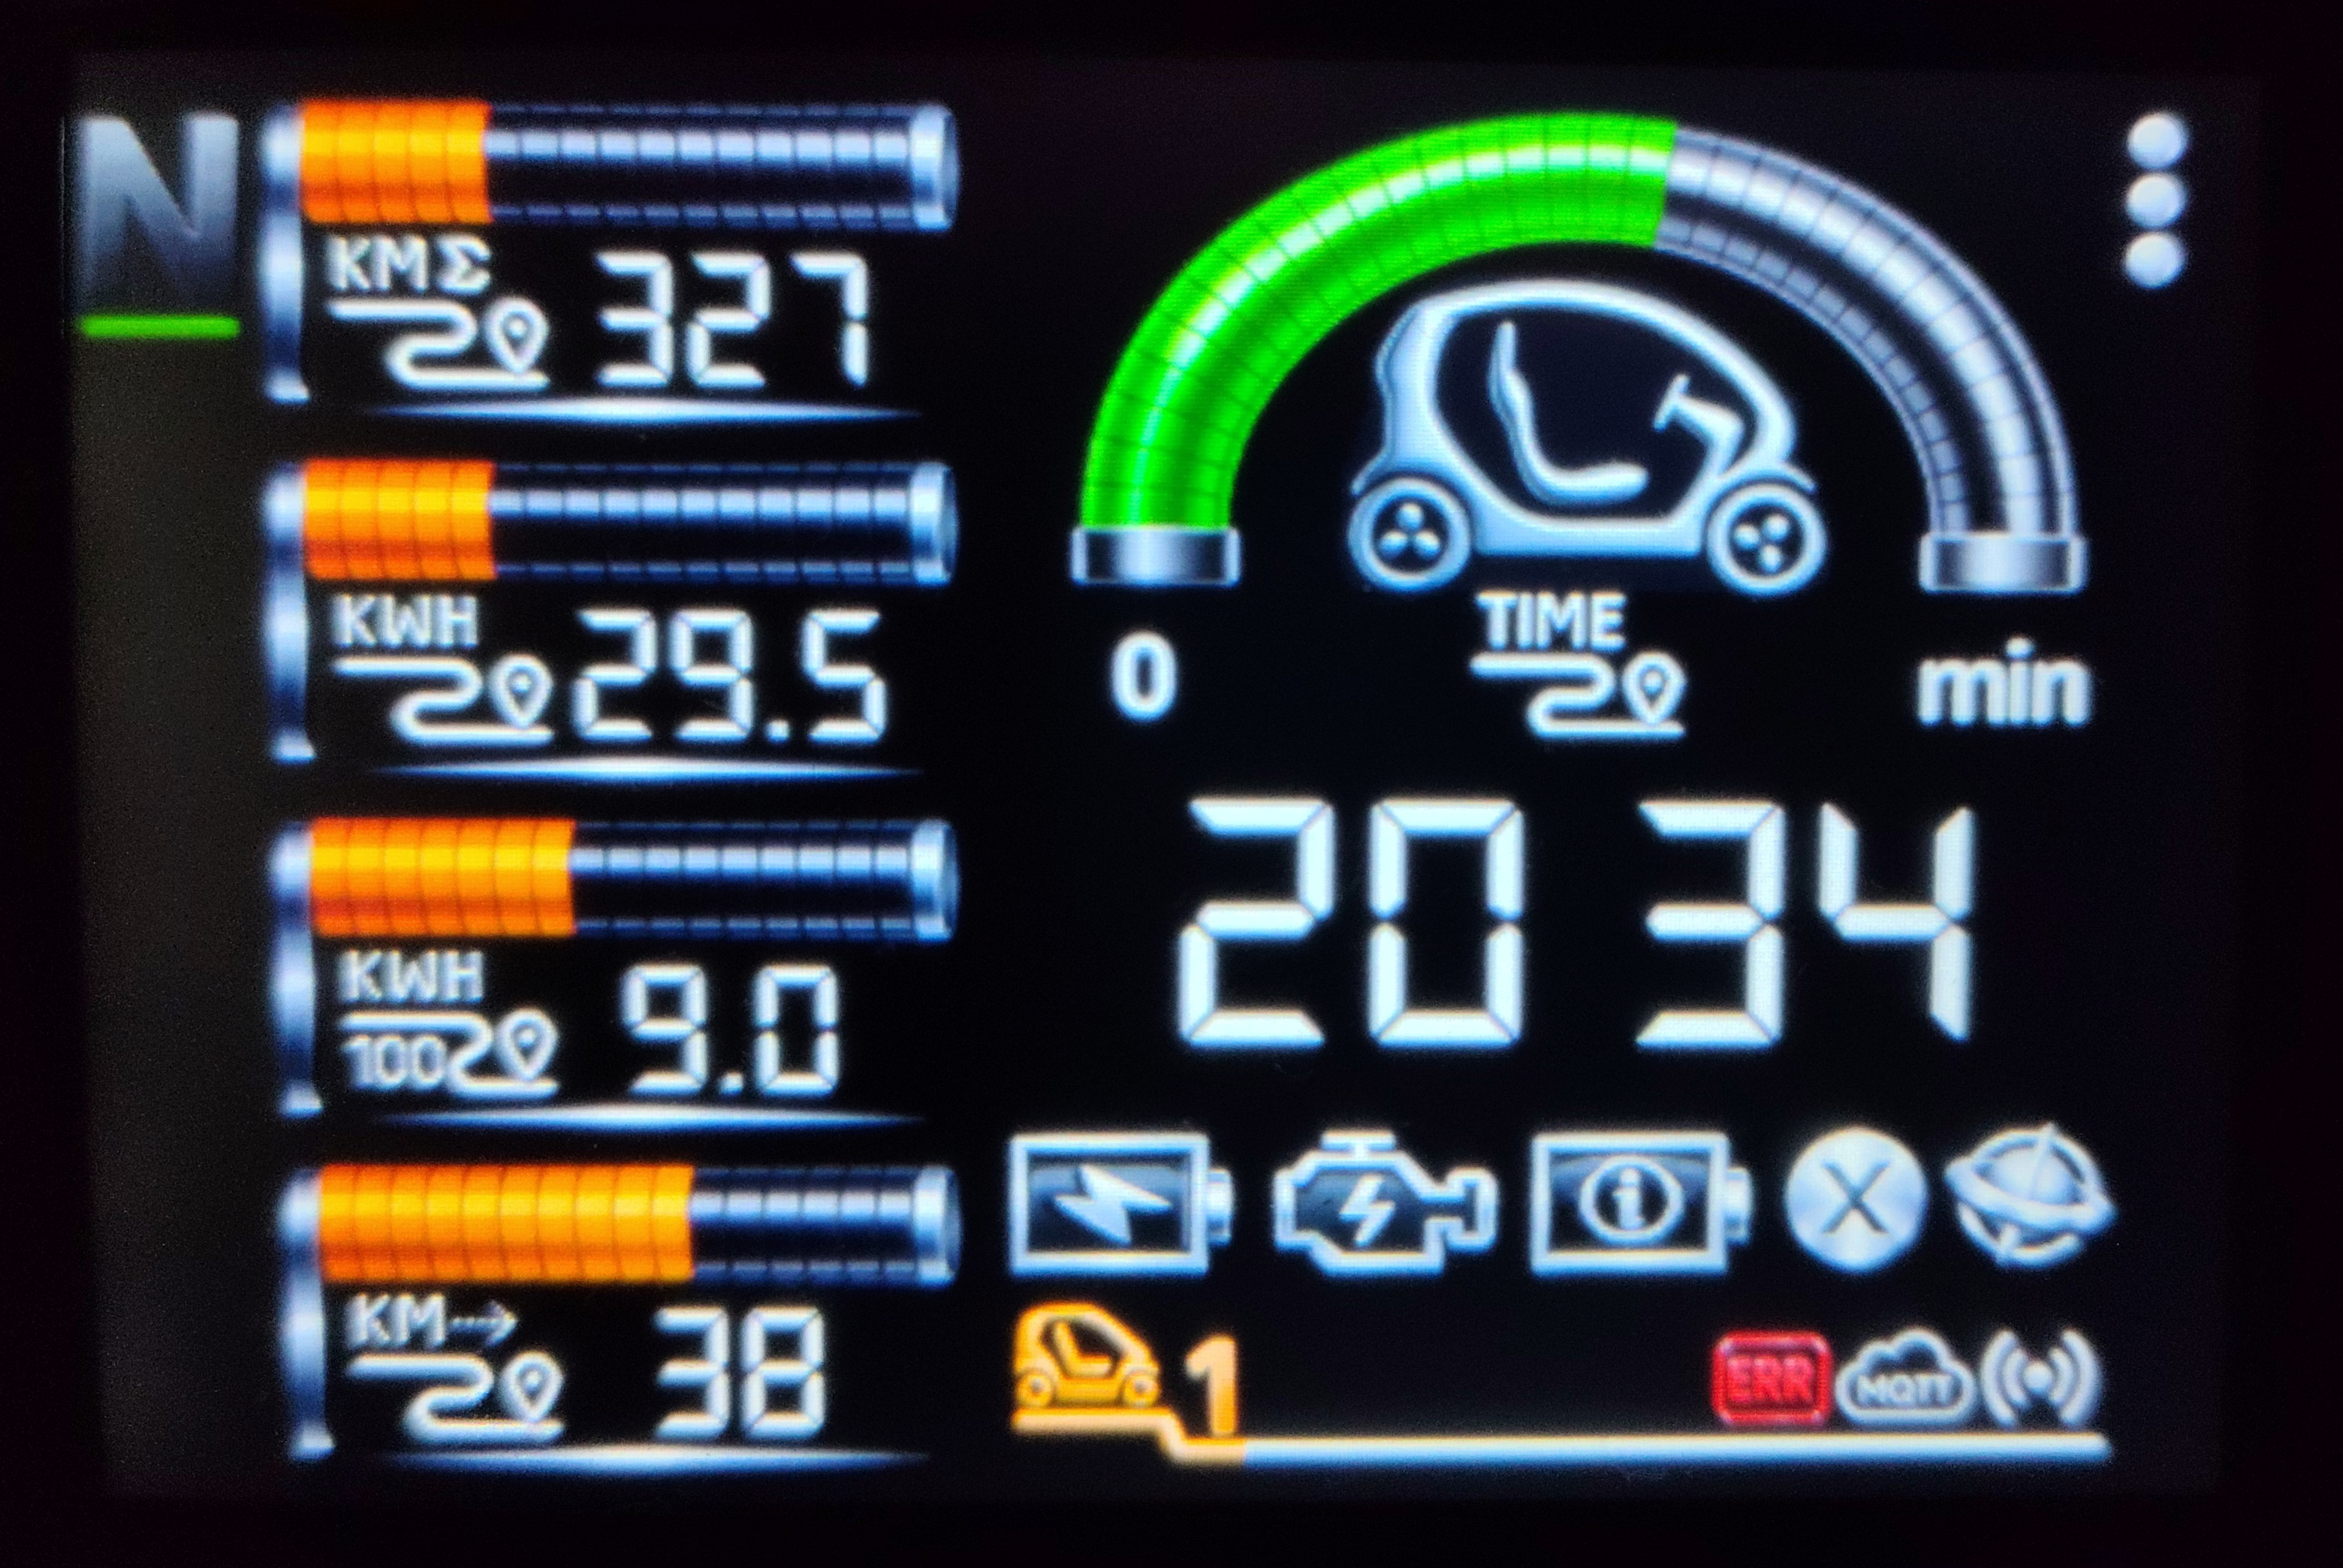
\includegraphics[width=0.8\textwidth]{figures/trip_page_full.jpg}
    \caption{Die Fahrt-Seite.}
\end{figure}

\subsection{Ändern der aktuellen Fahrt}

Wenn Sie mit der Aufzeichnung der Daten auf einer bestimmten Fahrt zwischen 1 und 5 beginnen möchten, können Sie das im vorherigen Bild gelb eingekreiste Fahrtsymbol drücken. Wenn Sie es zum ersten Mal drücken, gelangen Sie zur Fahrt Nr. 1 und wiederholtes Drücken durchläuft alle verfügbaren Fahrten, sodass Sie diejenige auswählen können, die Sie starten oder fortsetzen möchten.\\

Um zu sehen, in welcher Fahrt ToM derzeit aufzeichnet, beziehen Sie sich auf die orangefarbene Zahl im Fahrtsymbol. Sobald Sie die gewünschte Fahrt ausgewählt haben, können Sie bei Bedarf auch die aktive Seite wechseln, ohne die ausgewählte Fahrt zu verlieren, da ToM weiterhin Werte aufzeichnet, auch wenn die Fahrt-Seite nicht im Fokus steht.

\subsection{Fahrtaufzeichnung deaktivieren}

In diesem Beispiel befinde ich mich derzeit auf der Motorseite und zeichne Daten auf der fünften Fahrt-Seite auf, wie durch die kleine orangefarbene Zahl neben dem Fahrtsymbol angegeben. Wenn Sie die Fahrtaufzeichnung pausieren möchten, können Sie dies auf dem ToM+ tun, indem Sie \textbf{die Fahrttaste drei Sekunden lang gedrückt halten}, während eine andere Seite aktiv ist (in diesem Beispiel die Batterieseite).\\

\begin{figure}[ht]
    \centering

    \begin{subfigure}[t]{0.48\textwidth}
        \centering
        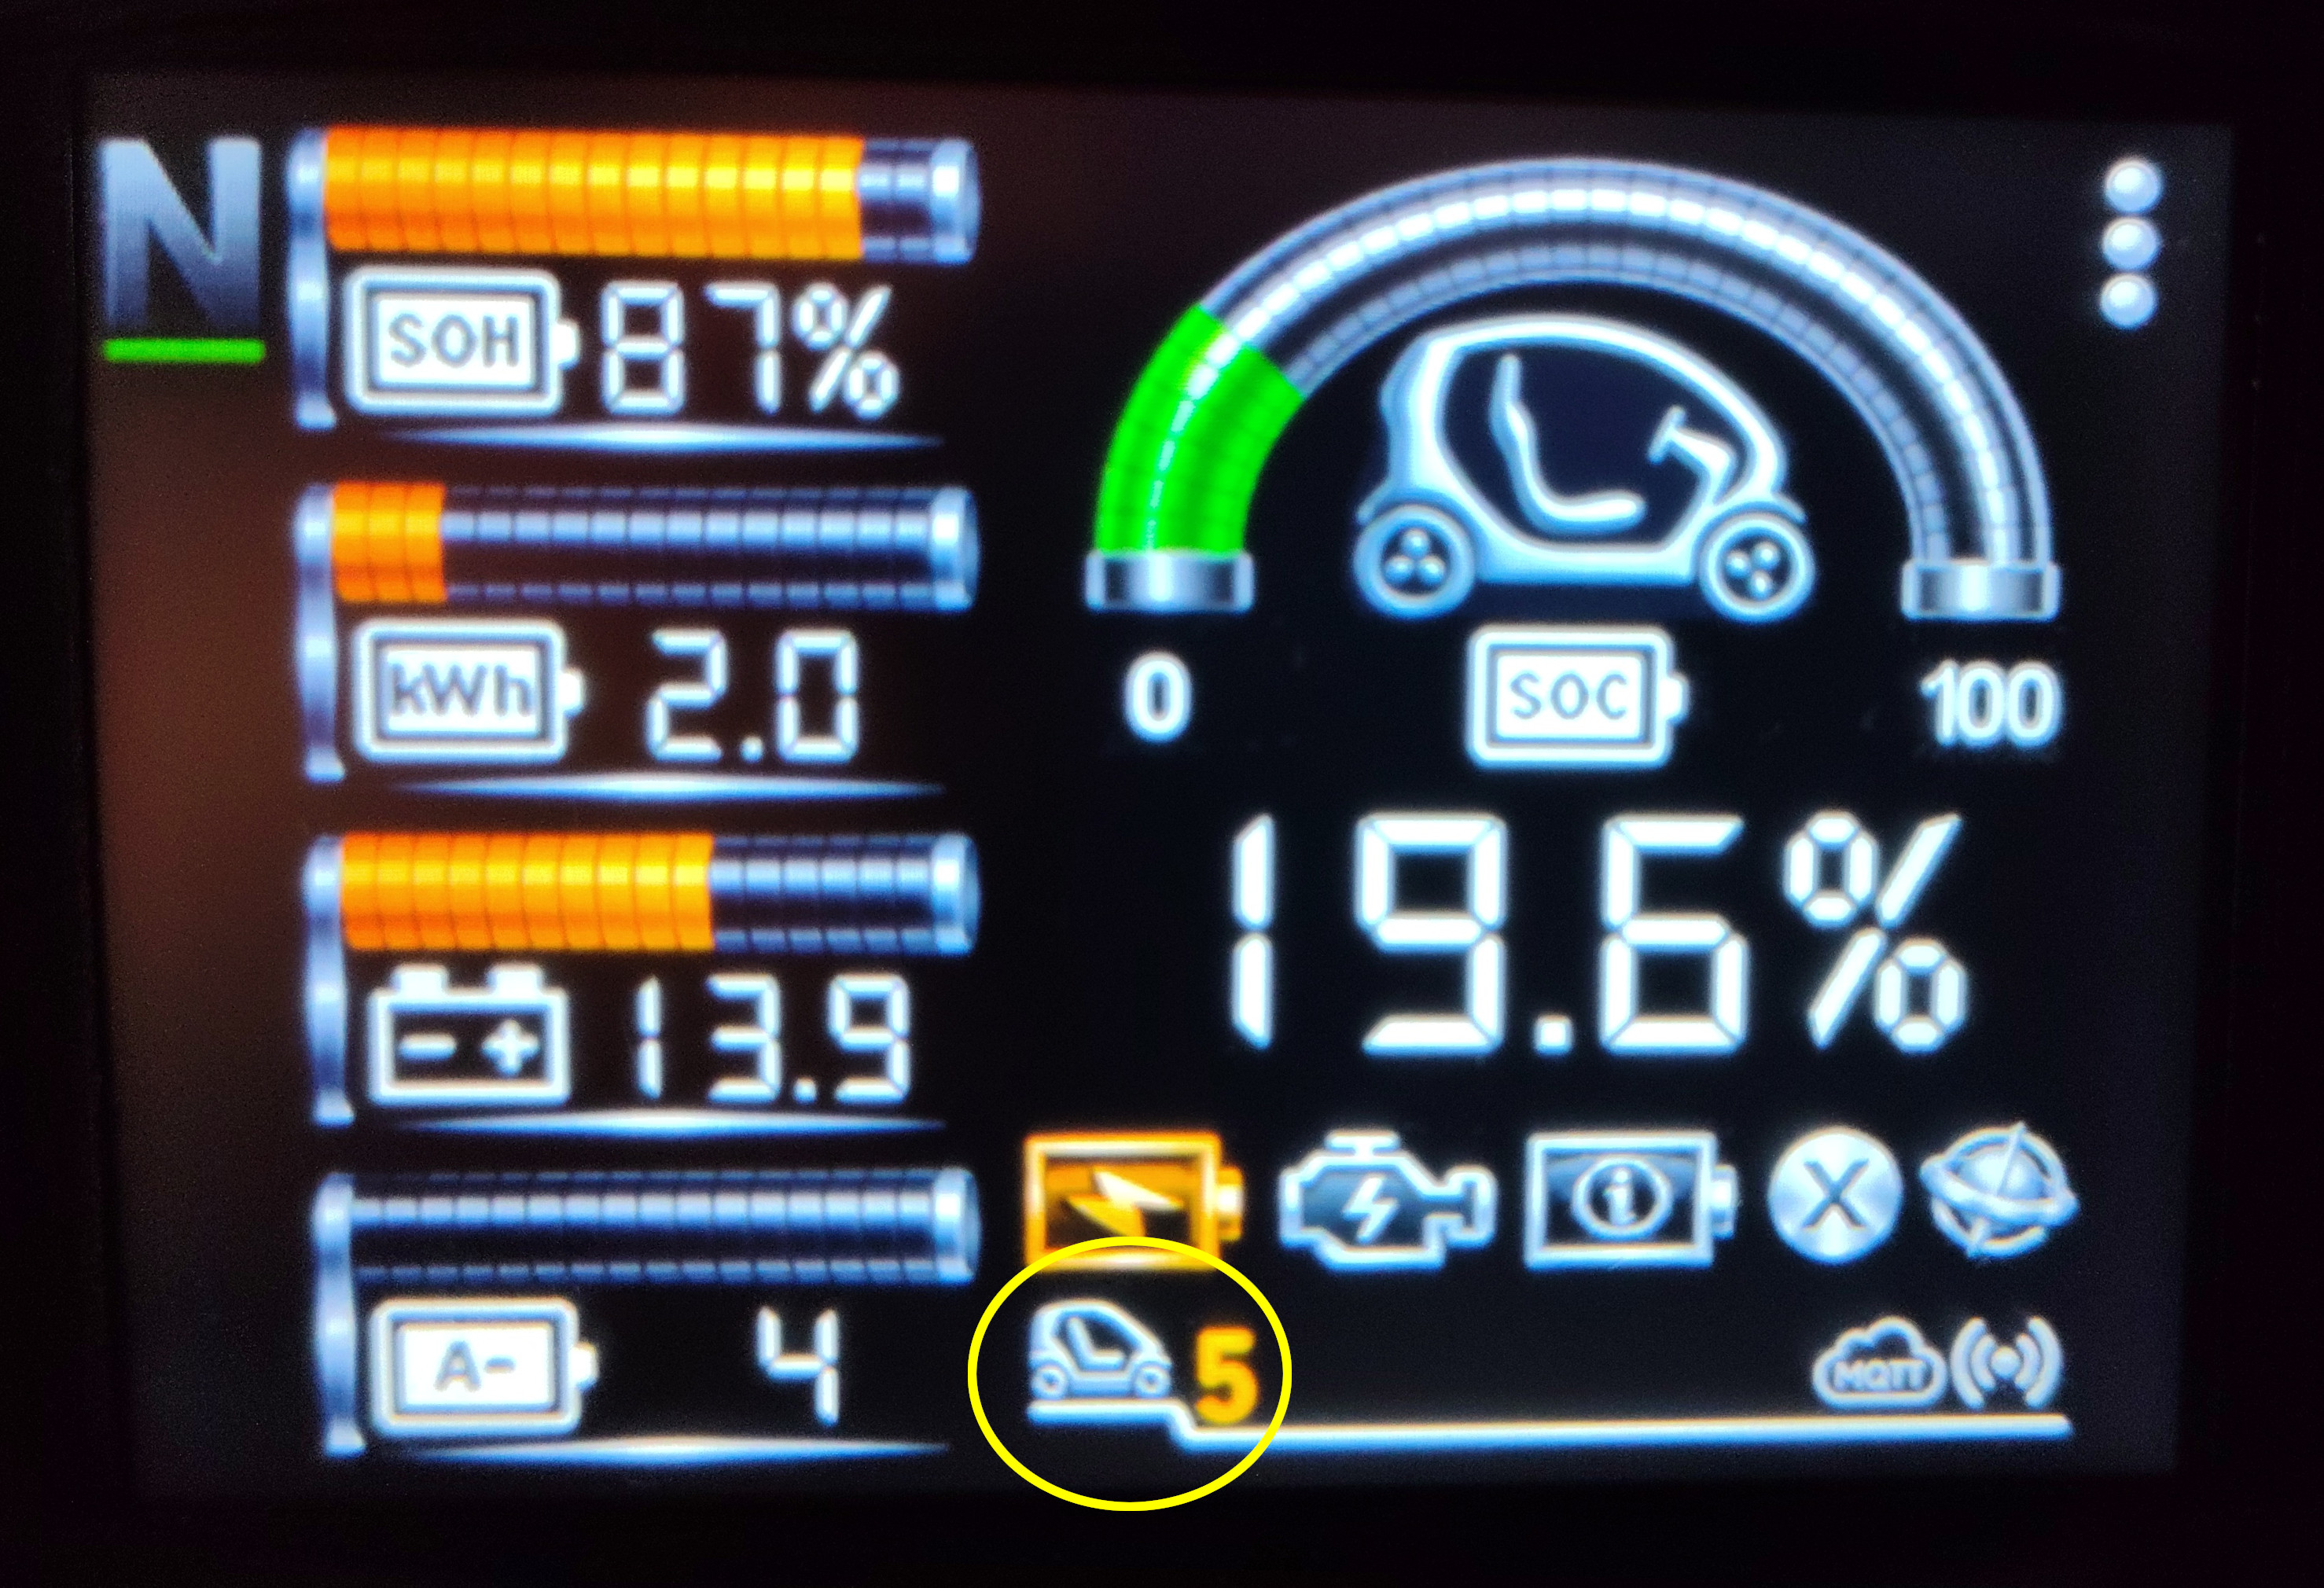
\includegraphics[width=\linewidth]{figures/trip_page_on.jpg}
        \caption{Fahrtaufzeichnung aktiv auf Fahrt 5.}
    \end{subfigure}
    \hfill
    \begin{subfigure}[t]{0.48\textwidth}
        \centering
        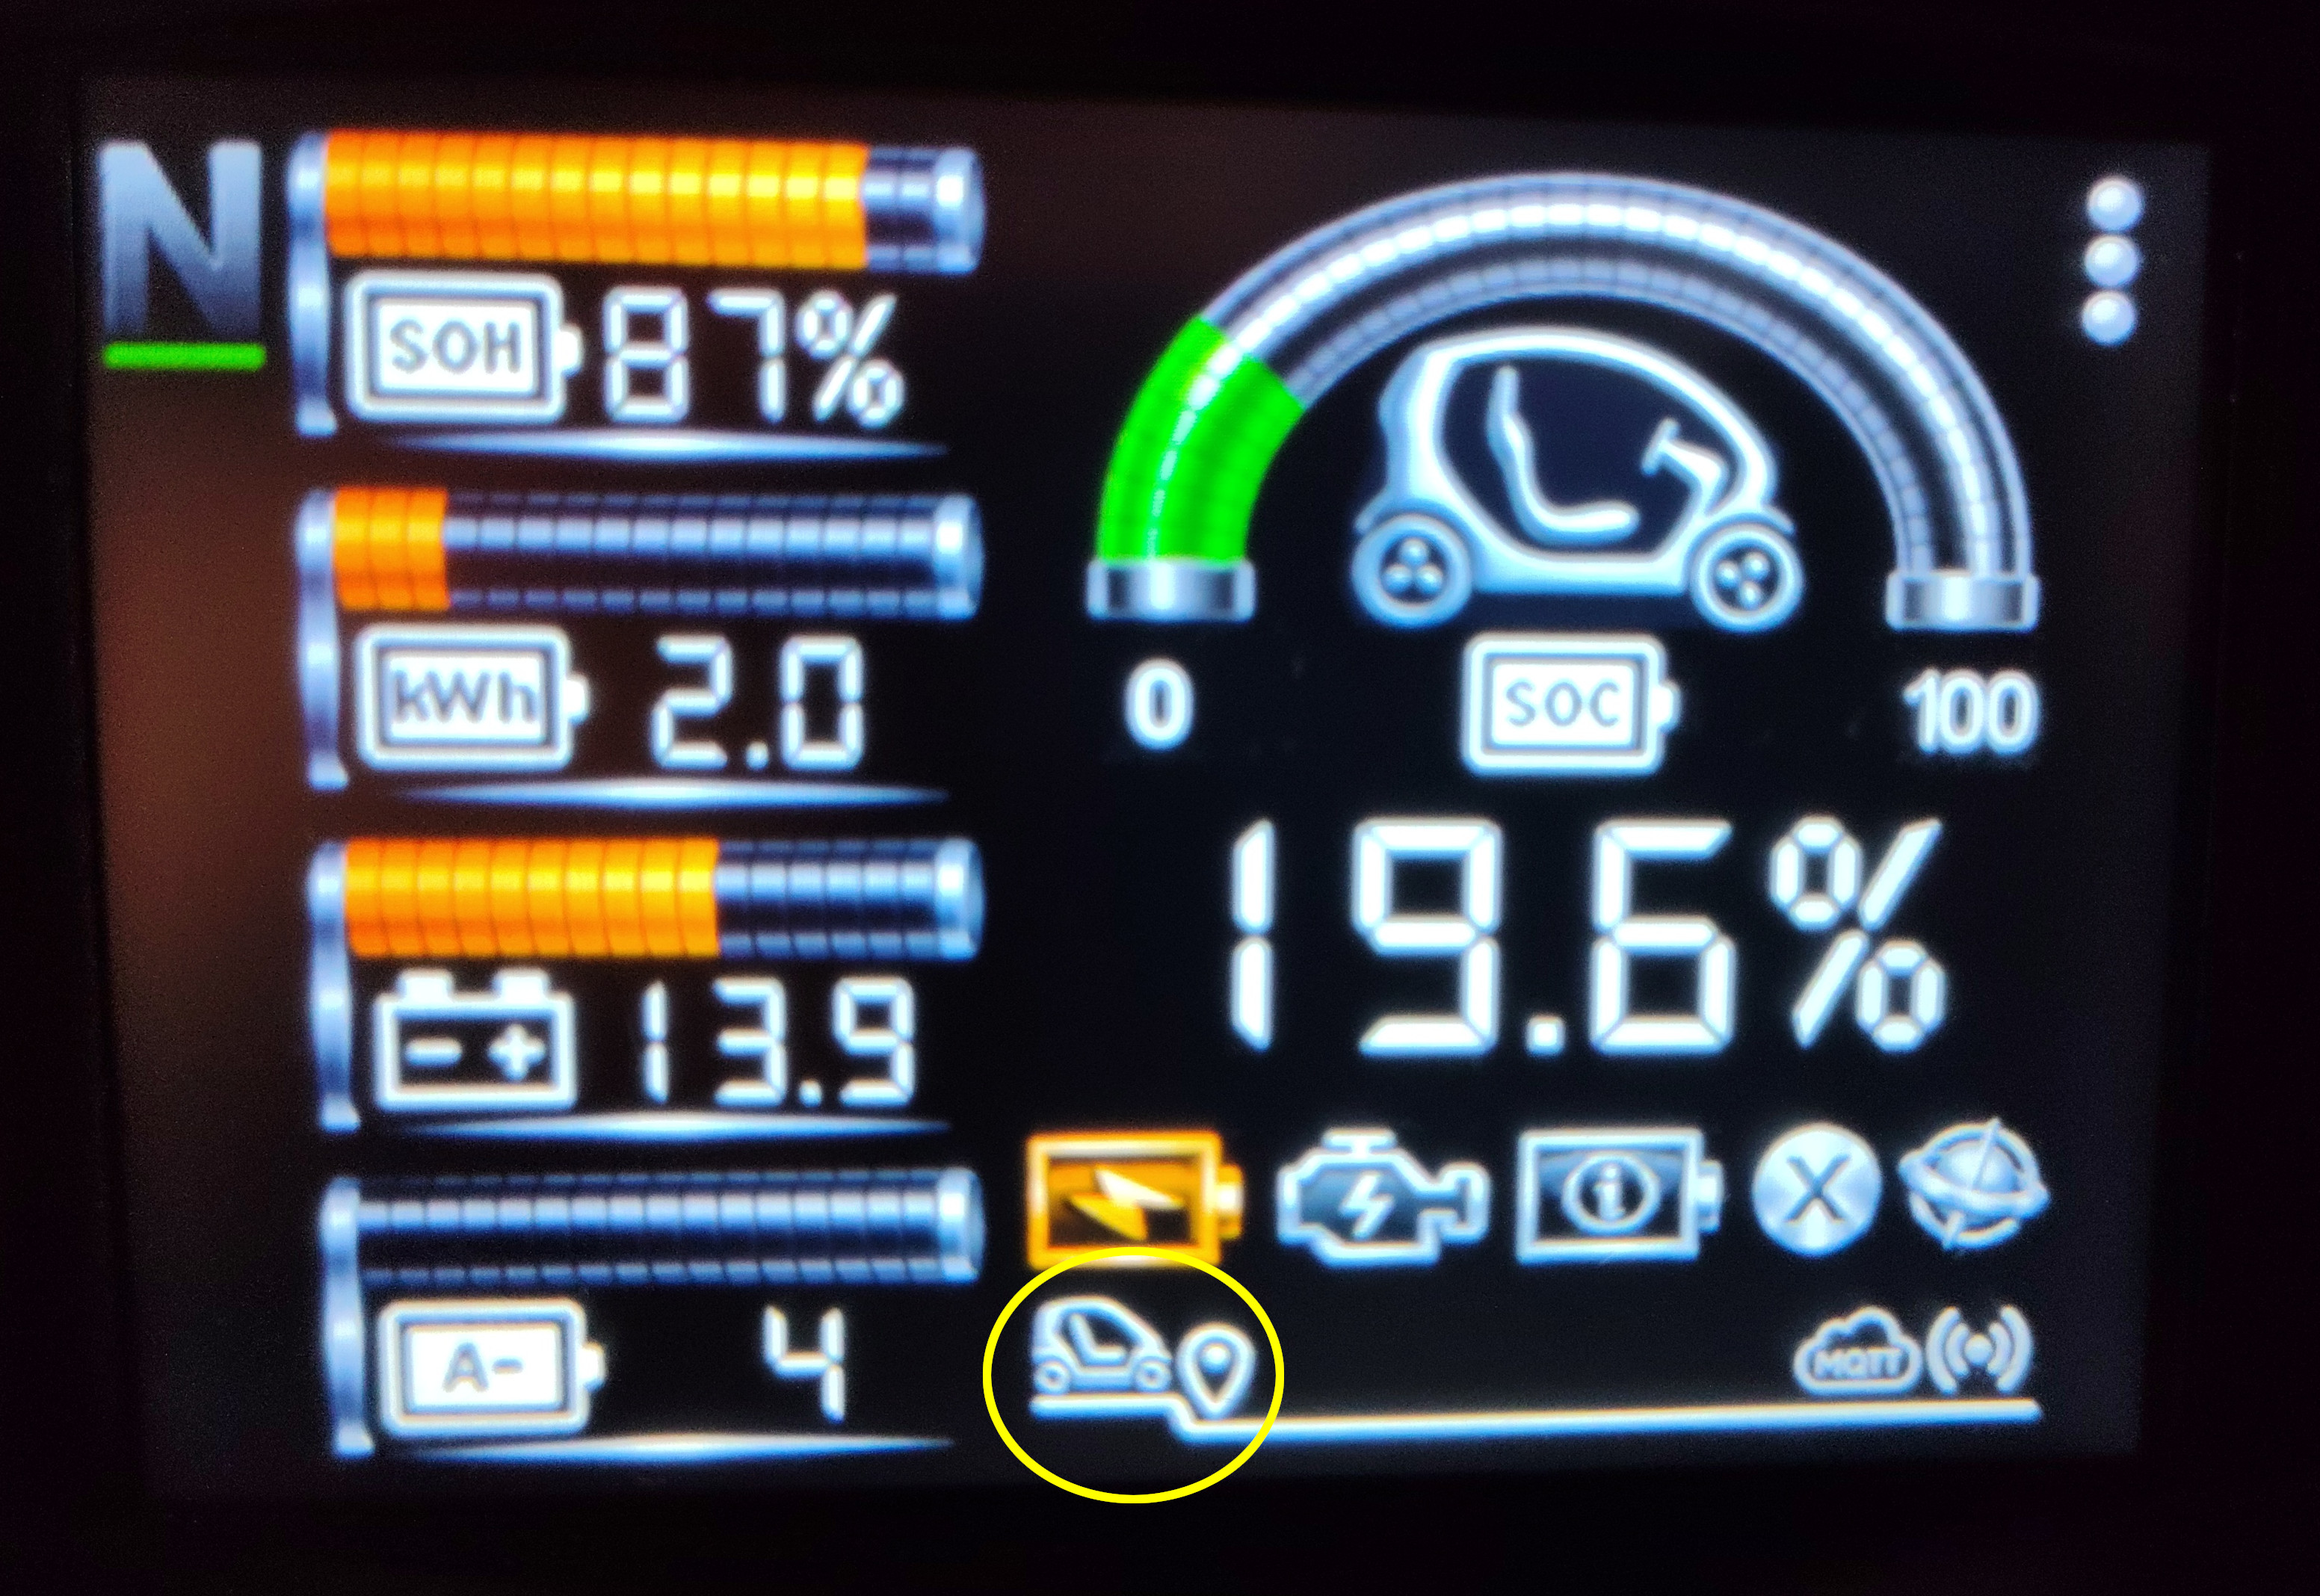
\includegraphics[width=\linewidth]{figures/trip_page_off.jpg}
        \caption{Fahrtaufzeichnung pausiert.}
    \end{subfigure}
\end{figure}

Sobald Sie losgelassen haben, ändert ToM+ das kleine Fahrtsymbol und zeigt das Kartensymbol anstelle der Fahrtnummer an, um Sie darüber zu informieren, dass keine Daten mehr aufgezeichnet werden (zweites Bild). Wenn Sie bereit sind, die Fahrt wieder aufzuzeichnen, drücken Sie auf die Fahrt-Seite, bis Sie die gewünschte Fahrt finden, indem Sie alle verfügbaren durchlaufen.

\subsection{Eine Fahrt zurücksetzen}

Wenn Sie eine bestimmte Fahrt löschen möchten, können Sie sie auswählen und \textbf{die Fahrttaste drei Sekunden lang gedrückt halten}. Sobald Sie losgelassen haben, sollten Sie feststellen, dass alle Fahrtwerte auf der Seite zurückgesetzt wurden (normalerweise auf Null). Der Unterschied zwischen dieser Aktion und der vorherigen besteht darin, dass in diesem Fall die Fahrtdaten gelöscht werden, während im vorherigen Fall die Fahrtdaten nur angehalten werden.
Außerdem müssen Sie sich hier auf der Fahrt-Seite befinden, während Sie sich im vorherigen Fall auf einer beliebigen anderen Seite befinden sollten.

\clearpage

\section{Die Fahrtenhistorie-Seite}
\label{sec:trip_history}

Diese Seite speichert die Daten der letzten zwanzig Fahrten und das Layout entspricht dem der Alarmprotokoll-Seite.
Die Werte werden nur aktualisiert und gespeichert, wenn die ausgewählte Fahrt die \textbf{Nummer 5} ist.

\subsection{So greifen Sie auf die Fahrtenhistorie-Seite zu}

Diese Seite ist von der Hauptseite aus nicht zugänglich, aber Sie können sie erreichen, indem Sie \textbf{das Alarmprotokoll-Symbol in der unteren Zeile des Bildschirms lange drücken}, bis es sich ändert. Dies liegt daran, dass die Fahrtenhistorie-Seite keine Seite ist, die Sie oft verwenden werden. Daher wurde beschlossen, sie aus Platzgründen vor der Hauptseite zu verbergen, ebenso wie die Fehlerseite. Die Abfolge der Seiten, die durch \textbf{langes Drücken des Alarmprotokoll-Symbols} verfügbar sind, lautet also:
Alarmprotokoll-Seite (Abschnitt~\ref{sec:alarm_log}) $\rightarrow$ Fehlerseite (Abschnitt~\ref{sec:error_page}) $\rightarrow$ Fahrtenhistorie-Seite $\rightarrow$ zurück zur Alarmprotokoll-Seite,
jeweils mit dem entsprechenden Symbol.\\

\begin{figure}[H]
    \centering
    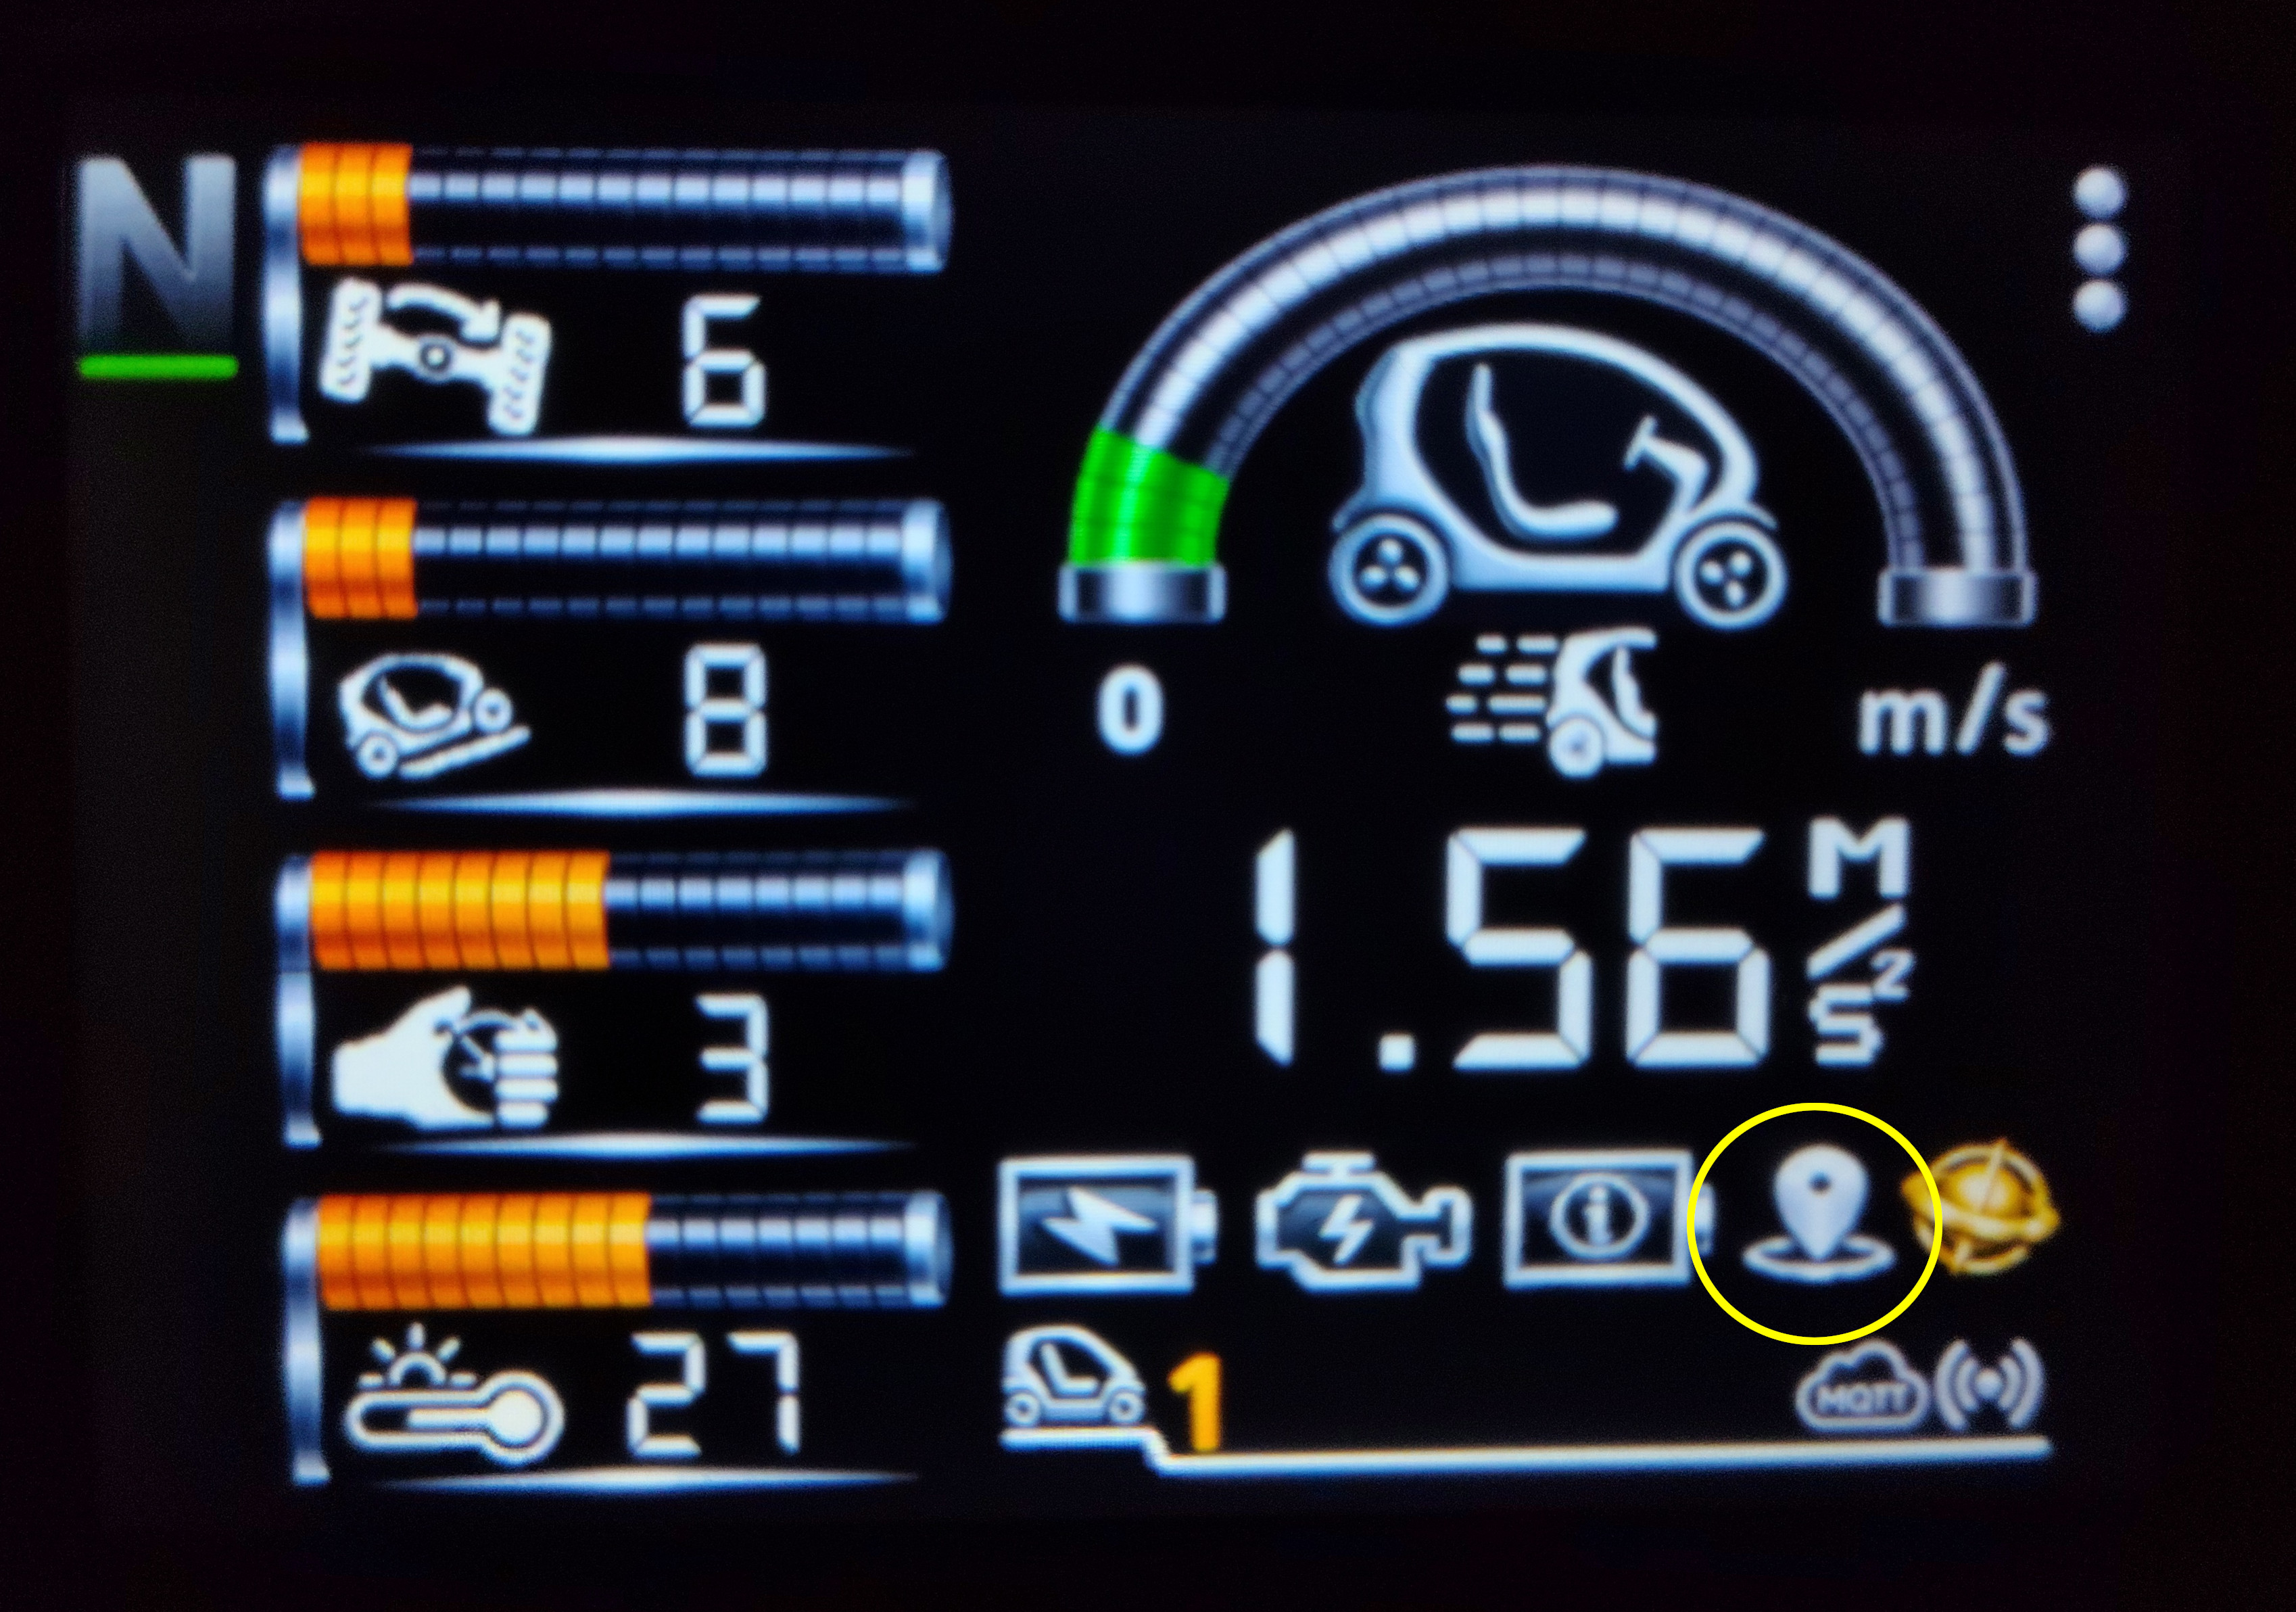
\includegraphics[width=0.8\textwidth]{figures/enter_trip_log_page.jpg}
    \caption{Das Symbol für den Zugriff auf die Fahrtenhistorie-Seite.}
\end{figure}

\subsection{Hauptsteuerelemente der Fahrtenhistorie-Seite}

\begin{figure}[H]
    \centering
    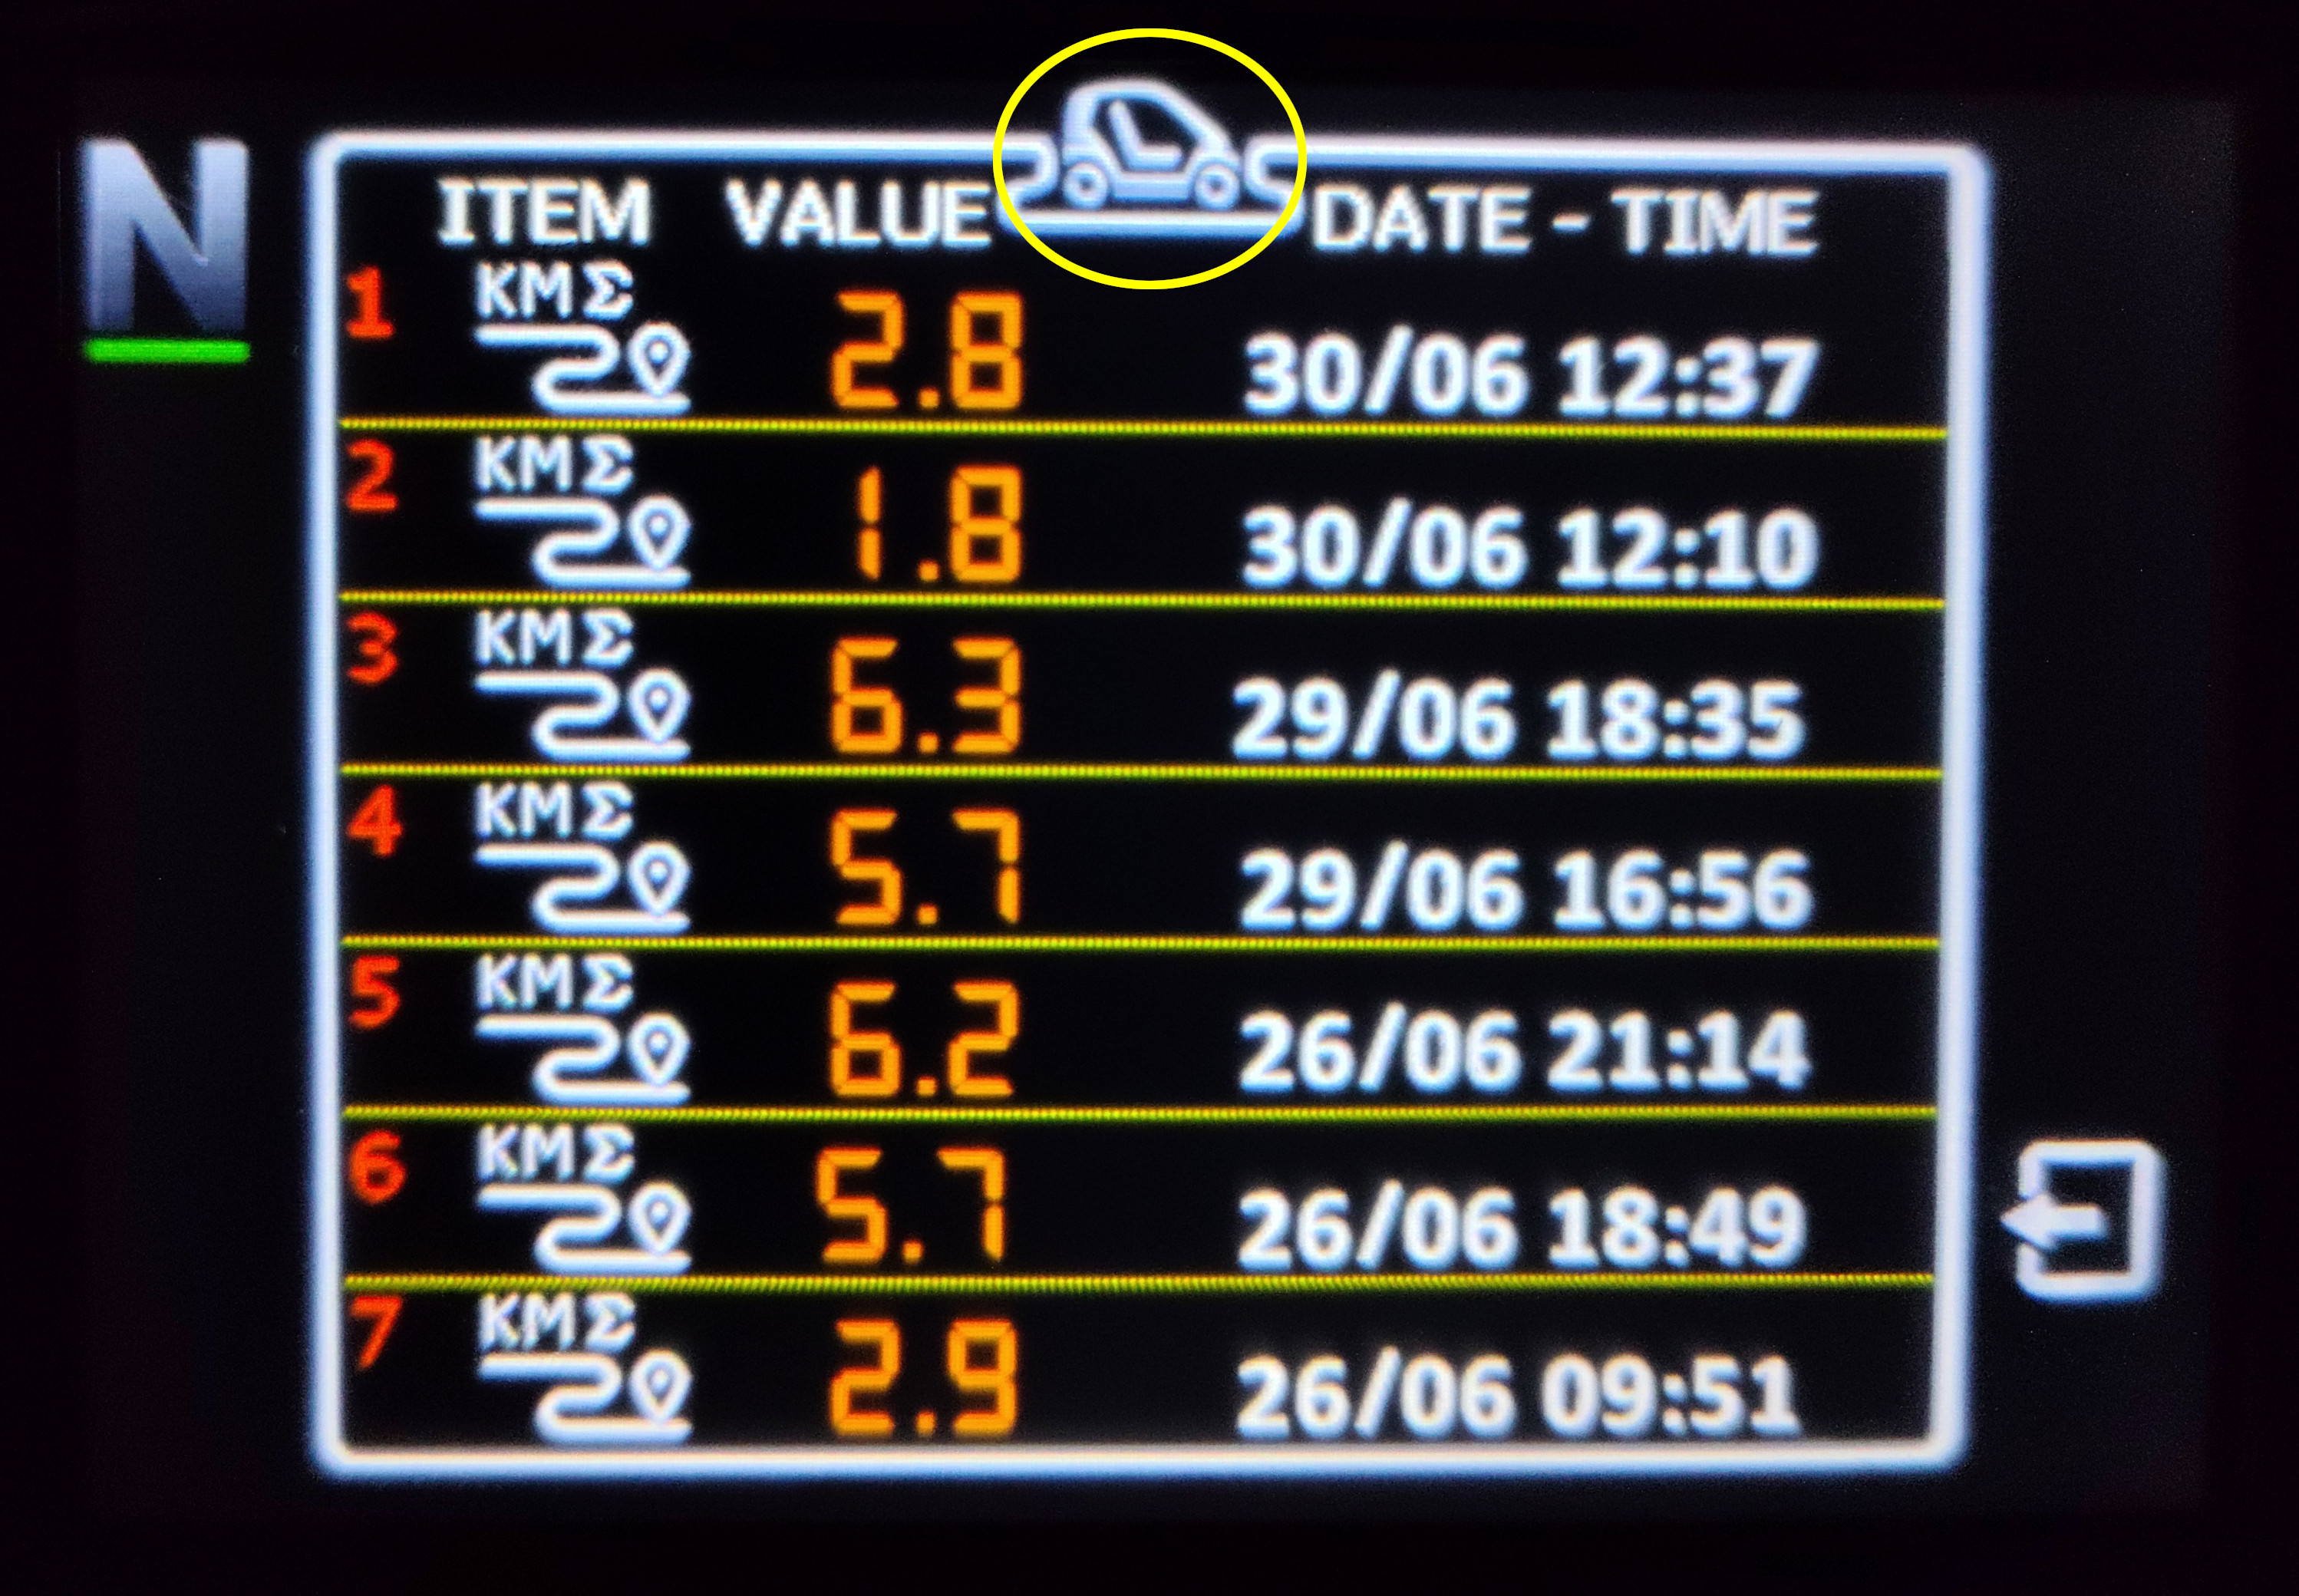
\includegraphics[width=0.8\textwidth]{figures/trip_history_page.jpg}
    \caption{Die Fahrtenhistorie-Seite.}
\end{figure}

Auf diesem Bild sehen Sie die ersten sieben Fahrten, die in der Liste gespeichert sind, mit Datum und Uhrzeit sowie der zurückgelegten Strecke.
Sie können die in jeder Zeile angezeigten Daten leicht ändern, indem Sie auf das Symbol der Daten drücken, wie unten gezeigt.
Die Daten wechseln zwischen den meisten verfügbaren Fahrtdaten, sodass Sie auswählen können, welche angezeigt werden sollen. 
In den nächsten Bildern sehen Sie dieselbe Seite mit dem Stromverbrauch der Fahrt und der Durchschnittsgeschwindigkeit.

\begin{figure}[ht]
    \centering

    \begin{subfigure}[t]{0.48\textwidth}
        \centering
        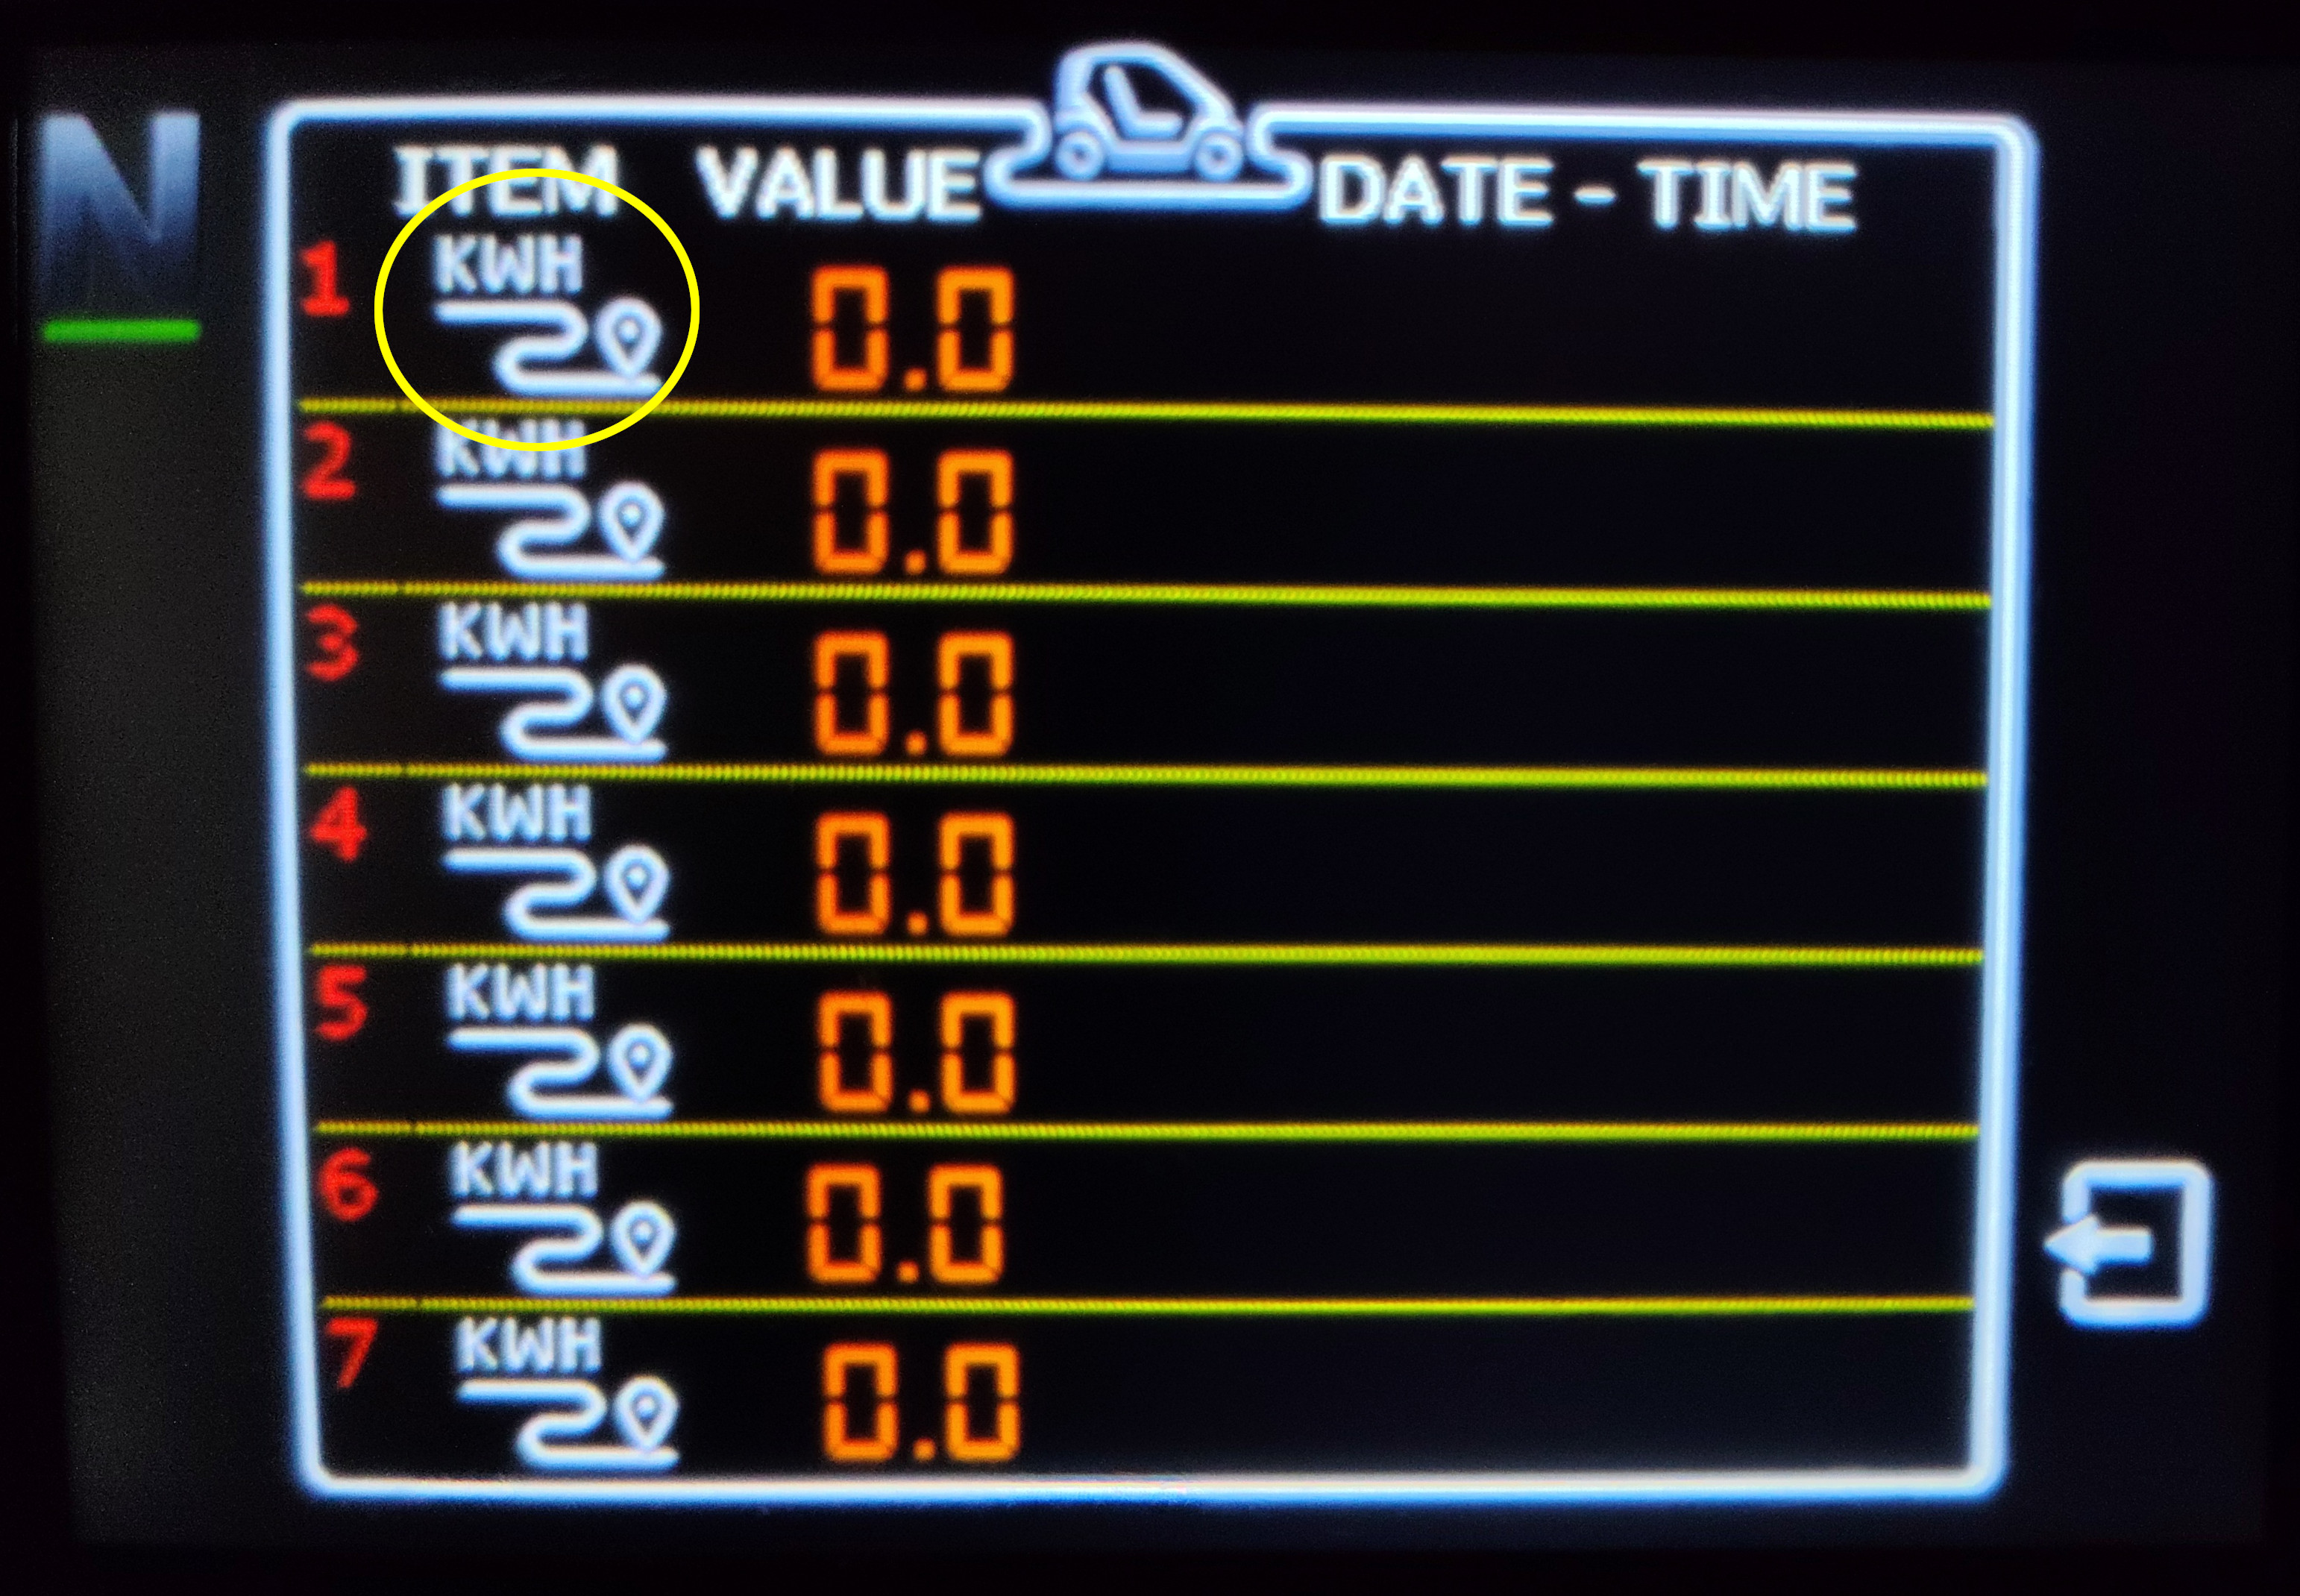
\includegraphics[width=\linewidth]{figures/trip_log_kwh.jpg}
        \caption{Fahrtstromverbrauch anzeigen.}
    \end{subfigure}
    \hfill
    \begin{subfigure}[t]{0.48\textwidth}
        \centering
        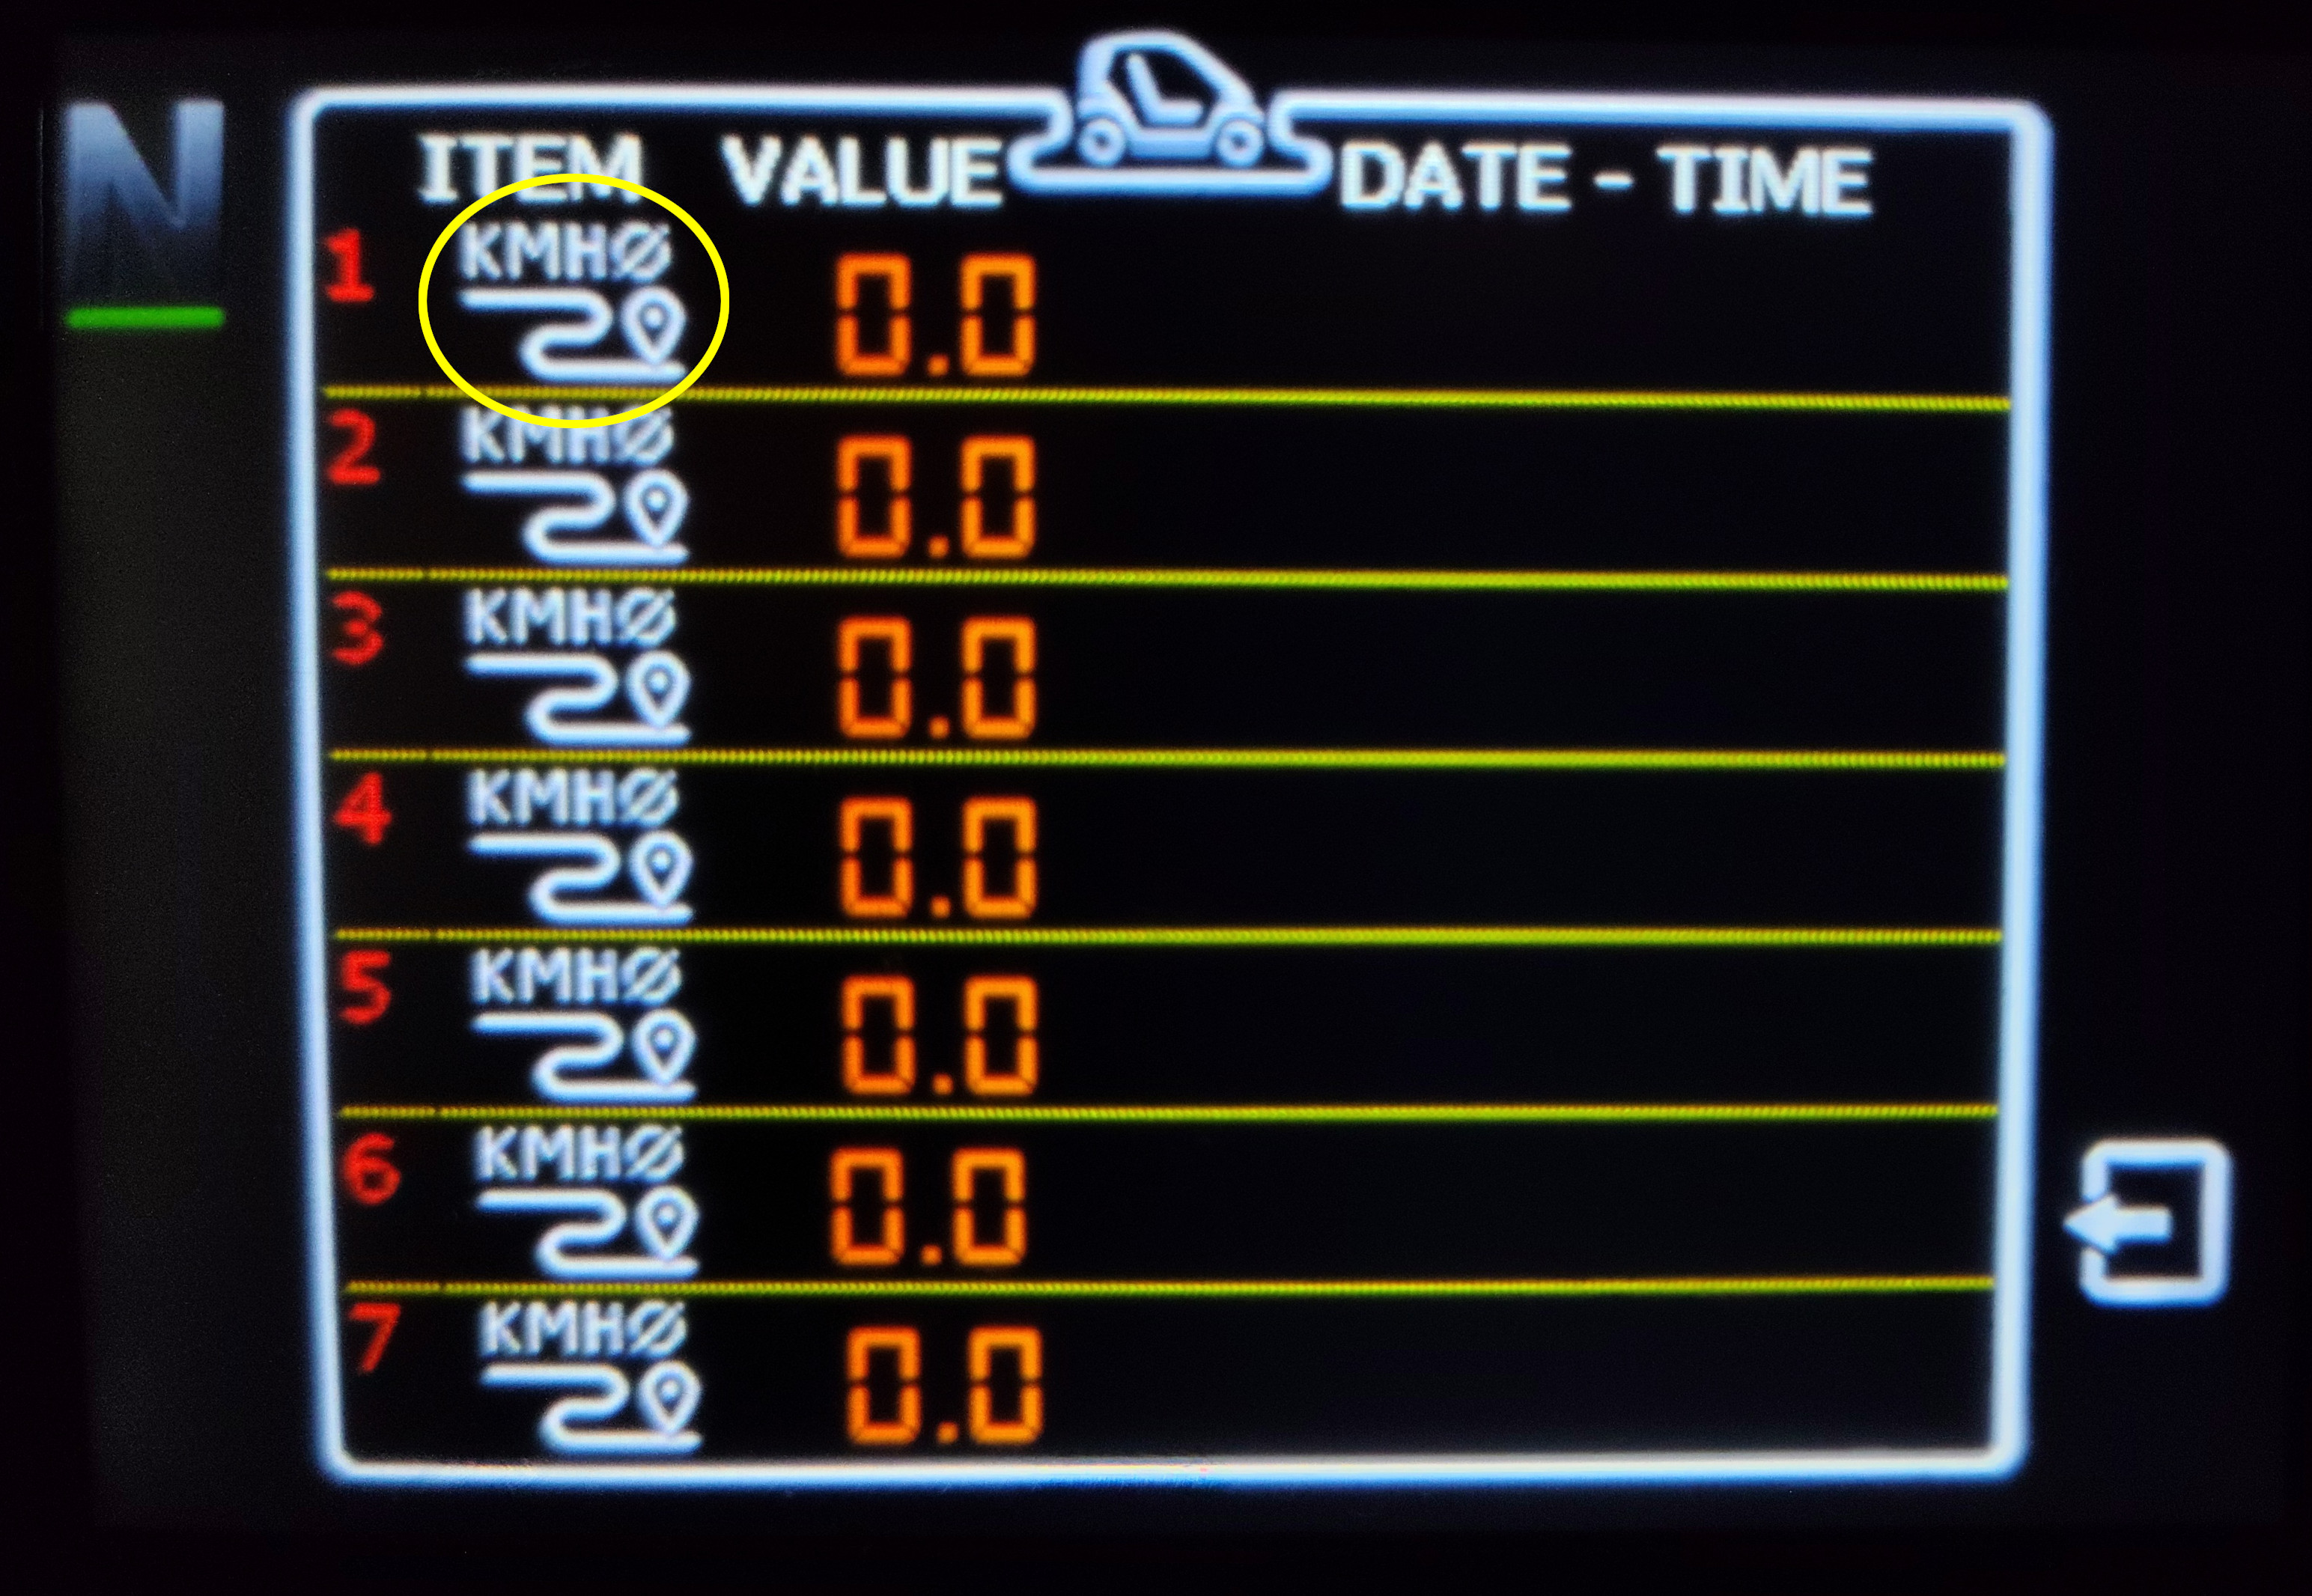
\includegraphics[width=\linewidth]{figures/trip_log_kmh.jpg}
        \caption{Durchschnittsgeschwindigkeit der Fahrt anzeigen.}
    \end{subfigure}
\end{figure}

Auf dem Webserver können Sie sie alle auf einmal sehen, dies wird in Abschnitt~\ref{sec:web_trip_history} besprochen.

\clearpage

\section{Die Fehlerseite}
\label{sec:error_page}

Diese Seite ähnelt der Alarmprotokoll-Seite und der Fahrtenhistorie-Seite, zeigt Ihnen jedoch die letzten aufgetretenen DTC-Fehler an.
Die Steuerelemente zum Löschen von Datensätzen oder zum Anzeigen älterer wurden bereits in Abschnitt~\ref{sec:alarm_log} besprochen.

\subsection{So greifen Sie auf die Fehlerseite zu}

Diese Seite ist nicht von der Hauptseite aus zugänglich, kann jedoch durch \textbf{langes Drücken des Alarmprotokoll-Symbols} in der unteren Zeile des Bildschirms erreicht werden, bis es sich ändert. Wie wir bereits besprochen haben, lautet die Abfolge der Seiten, die durch langes Drücken des Alarmprotokoll-Symbols verfügbar sind:
Alarmprotokoll-Seite (Abschnitt~\ref{sec:alarm_log}) $\rightarrow$ Fehlerseite $\rightarrow$ Fahrtenhistorie-Seite (Abschnitt~\ref{sec:trip_history}) $\rightarrow$ zurück zur Alarmprotokoll-Seite,
jeweils mit dem entsprechenden Symbol.\\

\begin{figure}[ht]
    \centering

    \begin{subfigure}[t]{0.48\textwidth}
        \centering
        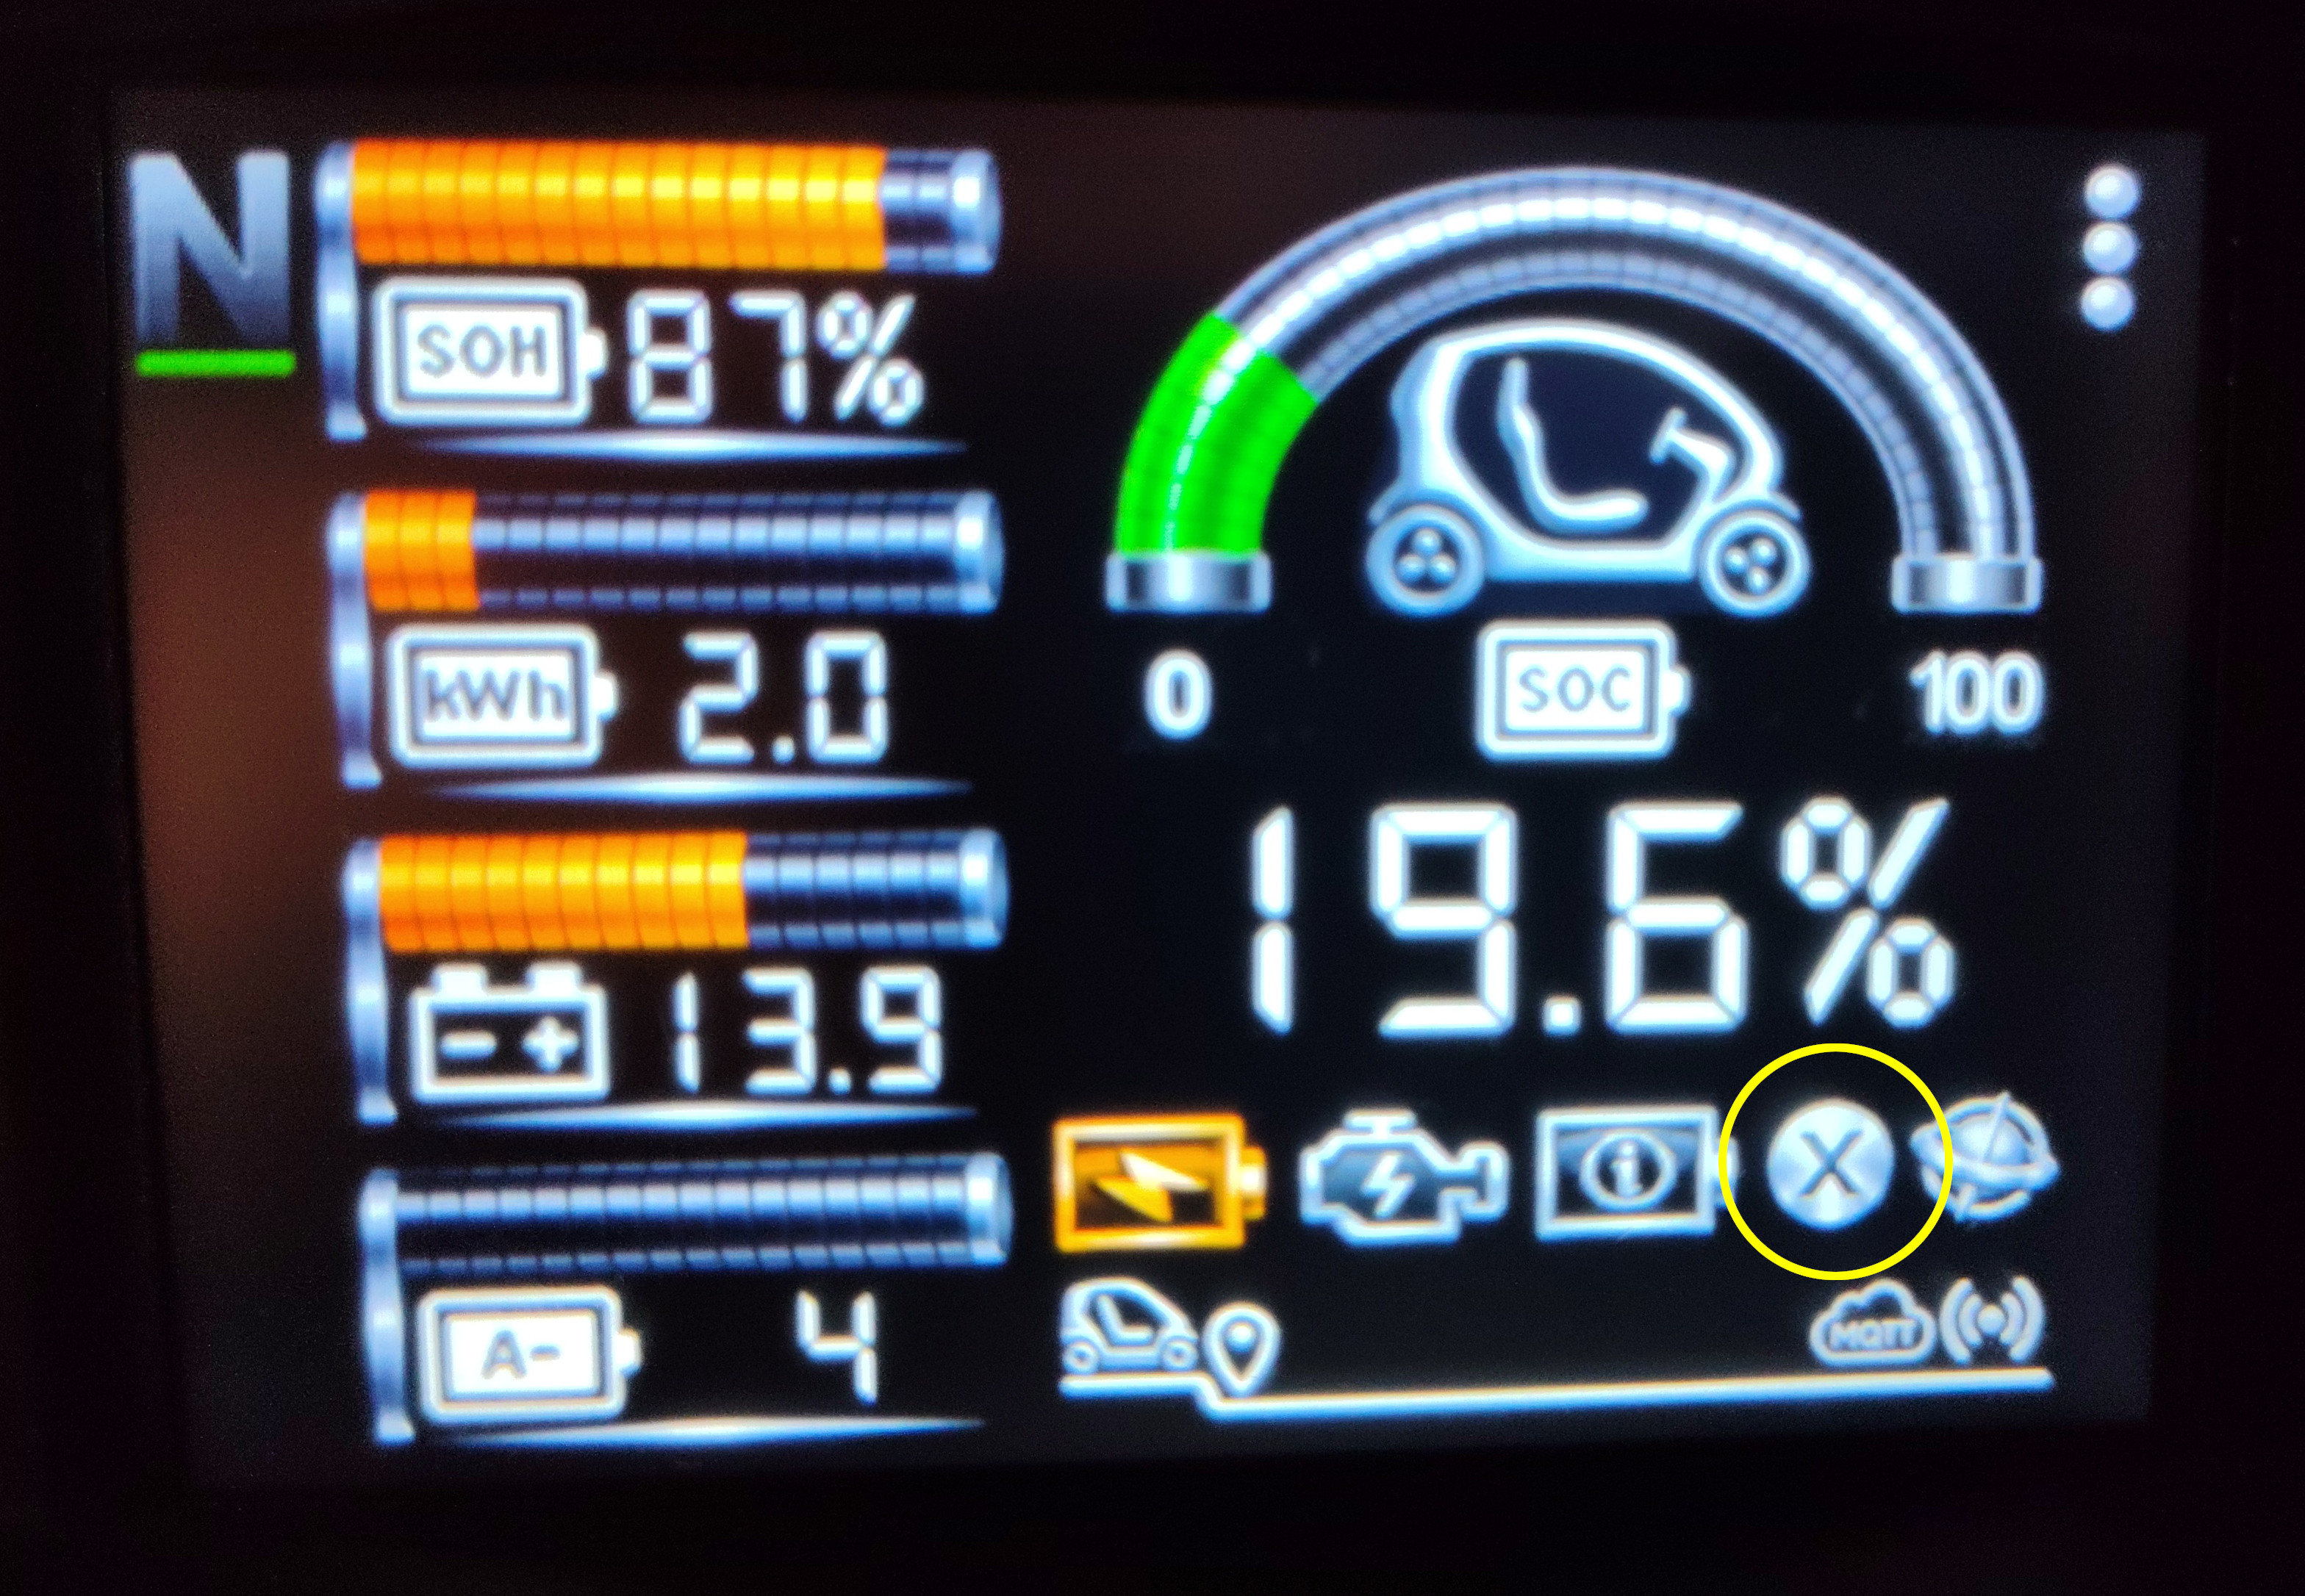
\includegraphics[width=\linewidth]{figures/enter_error_page.jpg}
        \caption{Das Symbol für den Zugriff auf die Fehlerseite.}
    \end{subfigure}
    \hfill
    \begin{subfigure}[t]{0.48\textwidth}
        \centering
        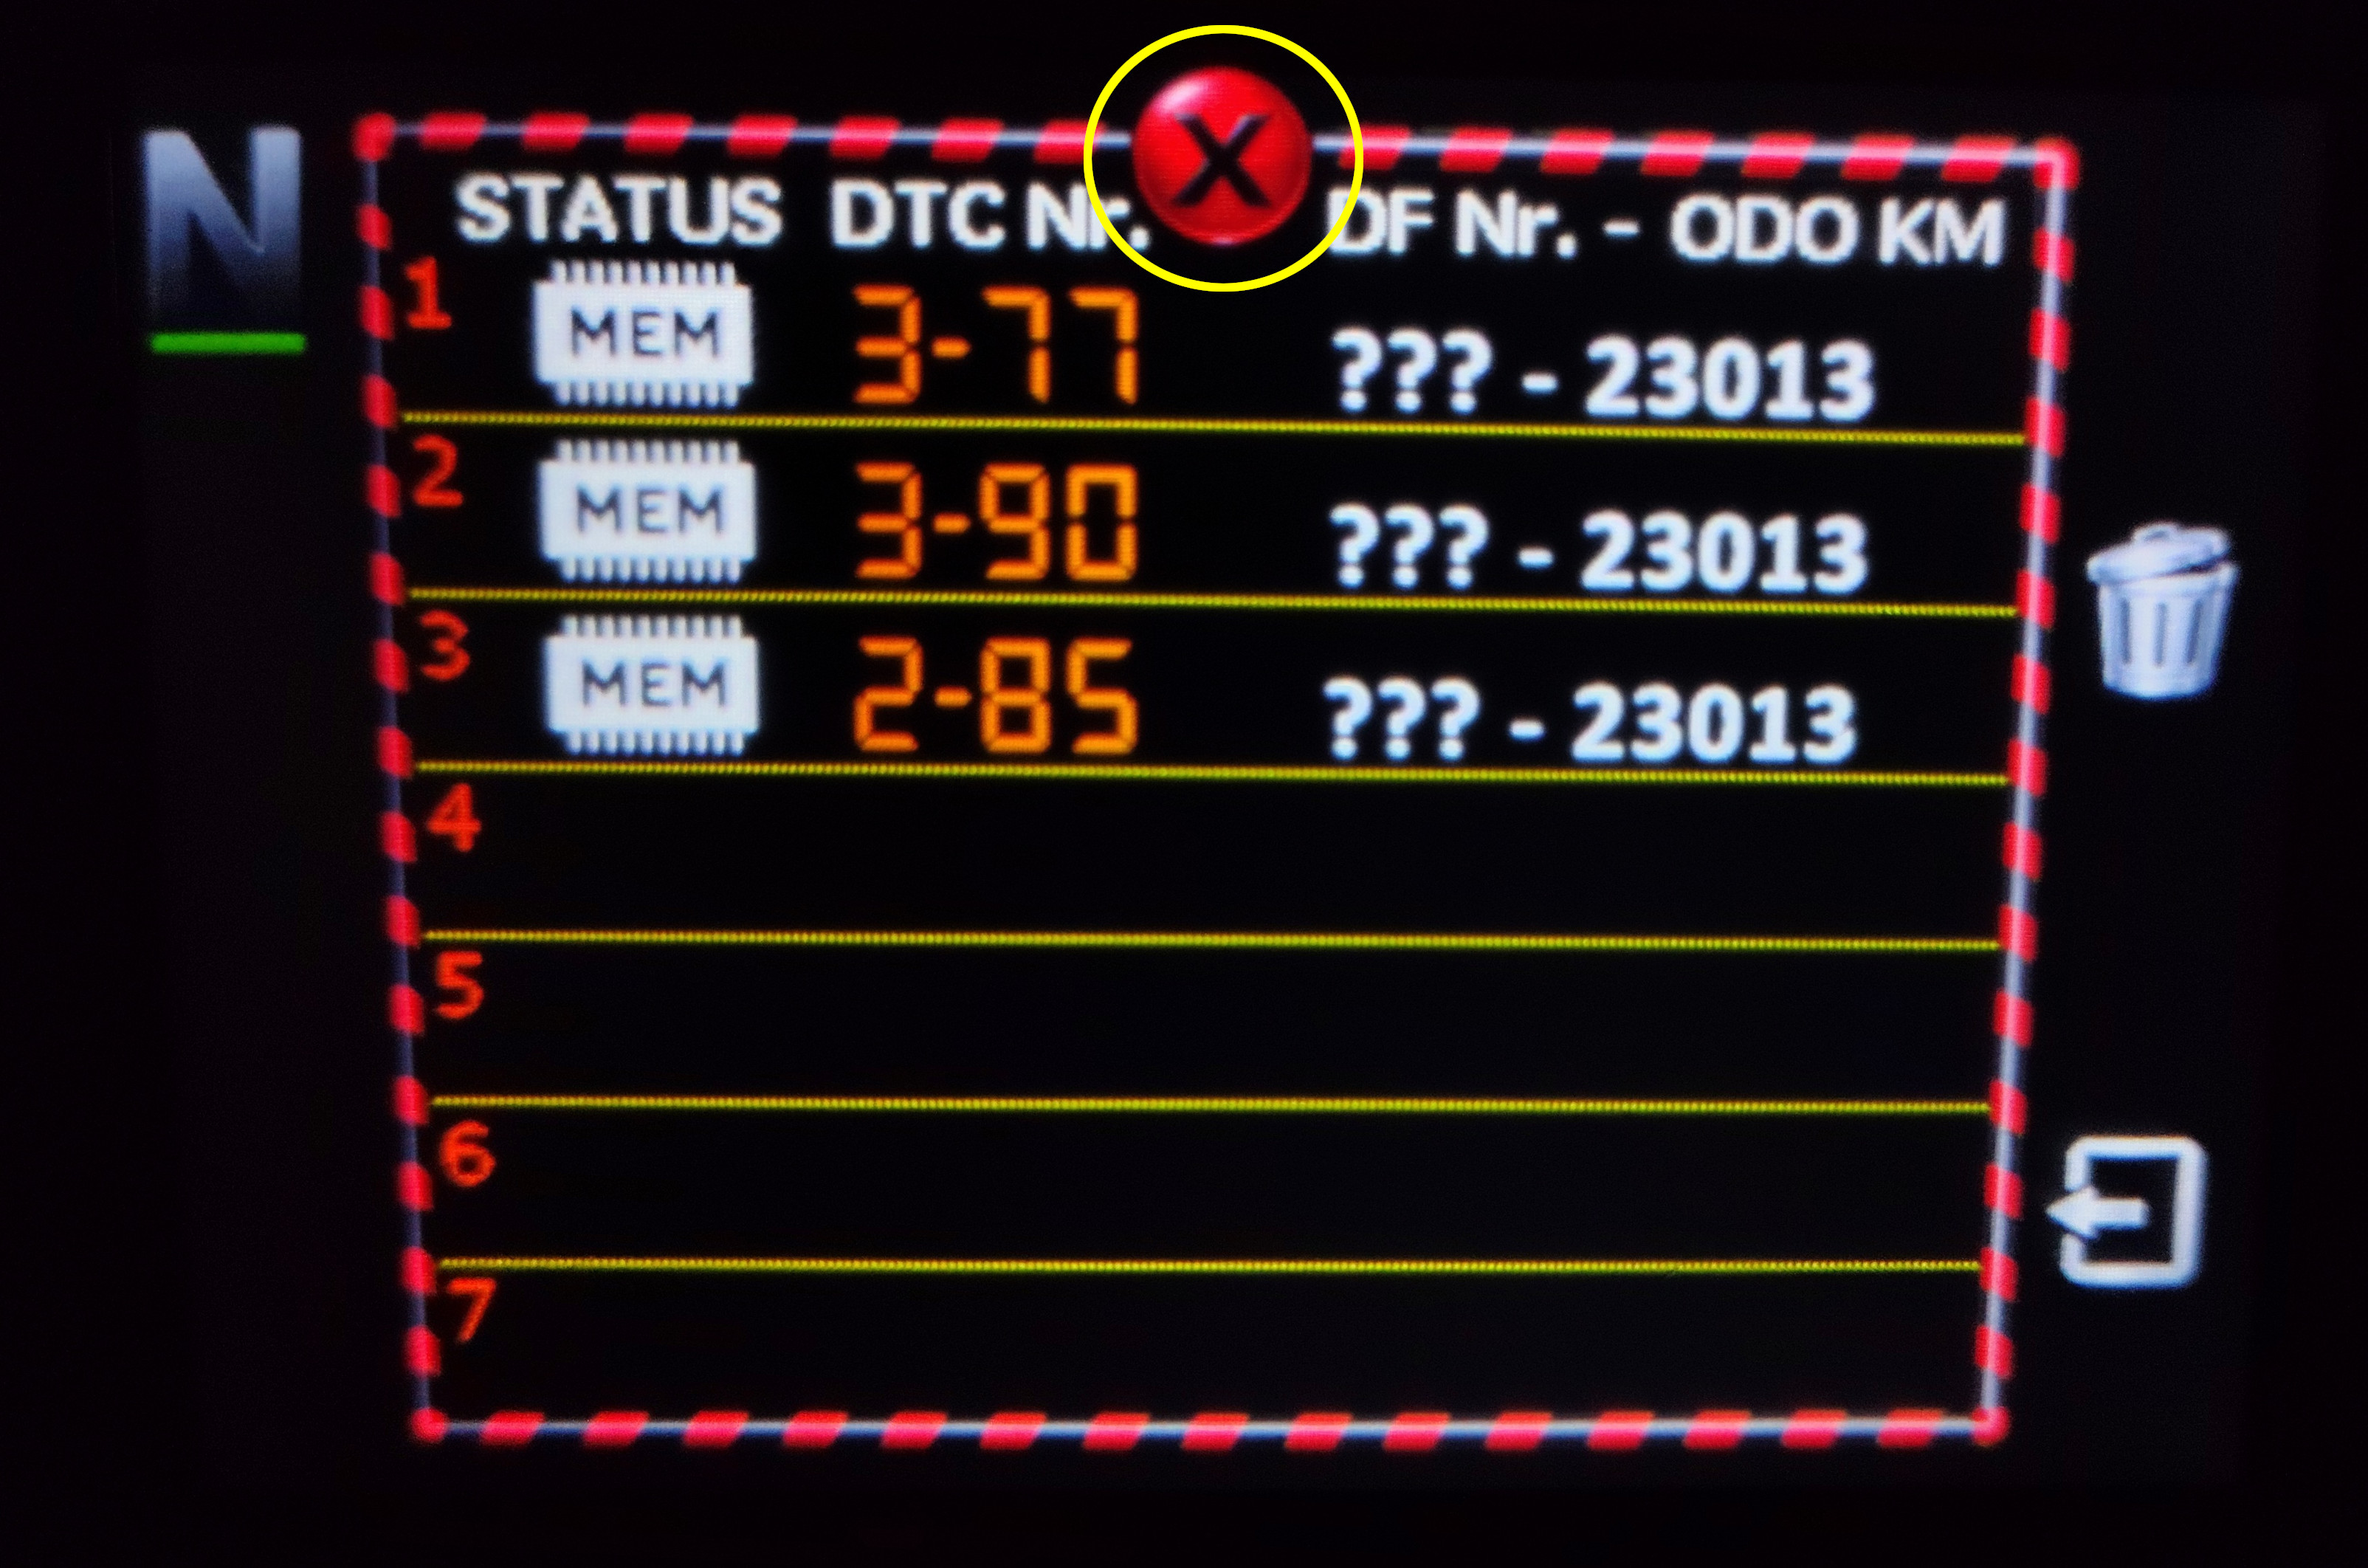
\includegraphics[width=\linewidth]{figures/error_page.jpg}
        \caption{Anzeigen der Fehlerseite.}
    \end{subfigure}
\end{figure}

\subsection{Hauptsteuerelemente der Fehlerseite}

Wie Sie im zweiten Bild oben sehen können, ähnelt die Fehlerseite der Alarmprotokoll-Seite. 
Es wird eine Liste der letzten 14 aufgetretenen Fehler angezeigt, mit ihrem ODO, der DTC-Nummer,
der DF-Nummer (falls verfügbar) und einem repräsentativen Symbol. Weitere Informationen wie SOC, Geschwindigkeit und eine kurze Beschreibung finden Sie auf der entsprechenden Seite des Webservers (Abschnitt~\ref{sec:web_diagnostic}).\\

Durch Drücken auf das Symbol des Fehlers (im Bild gelb eingekreist) können Sie durch die Seiten der gespeicherten Fehler blättern,
welche insgesamt 14 betragen. Die erste Seite zeigt die letzten 7 Fehler, während die zweite Seite die älteren zeigt.
Um \textbf{Fehleraufzeichnungen zu löschen}, sowohl auf dieser Seite als auch im Auto, klicken Sie einfach auf das Mülleimer-Symbol.\\

Wie auf anderen Seiten reichte der Platz nicht aus, um die Schaltflächen zum Seitenwechsel einzufügen. Daher können Sie die Beenden-Schaltfläche in der unteren rechten Ecke drücken, um zur vorherigen Seite zurückzukehren, und dann bei Bedarf die aktive Seite wechseln.

\clearpage

\section{Die Ladeseite}
\label{sec:charging_page}

Diese Seite wird während der Fahrt nicht angezeigt und es gibt keine spezielle Schaltfläche, um sie aufzurufen. Das
liegt hauptsächlich daran, dass dieser Ladebildschirm automatisch angezeigt wird, wenn sich der Twizy gerade im Ladezustand befindet. 

Wie Sie auf dem Bild sehen können, ist das Layout dasselbe wie auf der Armaturenbrett-Seite. Der aktuelle
SOC wird in der Mitte angezeigt und ersetzt den Geschwindigkeitswert.\\

Es wird auch eine Animation gestartet, deren Geschwindigkeit je nach Ladeleistung variiert.
Auf dem Foto unten gibt es auch einige ladespezifische Daten, die Sie in den Einstellungen
ändern können, wie später erklärt wird. Auf dieser Seite haben Sie nicht die Symbol-Statusleiste, aber Sie haben immer noch
die Netzwerkstatus-Symbole in der unteren rechten Ecke, da Sie die Ladewerte Ihres Autos auch überwachen können,
wenn das Auto ausgeschaltet ist. Tatsächlich schaltet sich das ToM+ automatisch ein, wenn Sie Ihren
Twizy an eine gültige Stromversorgung anschließen.

\begin{figure}[H]
    \centering
    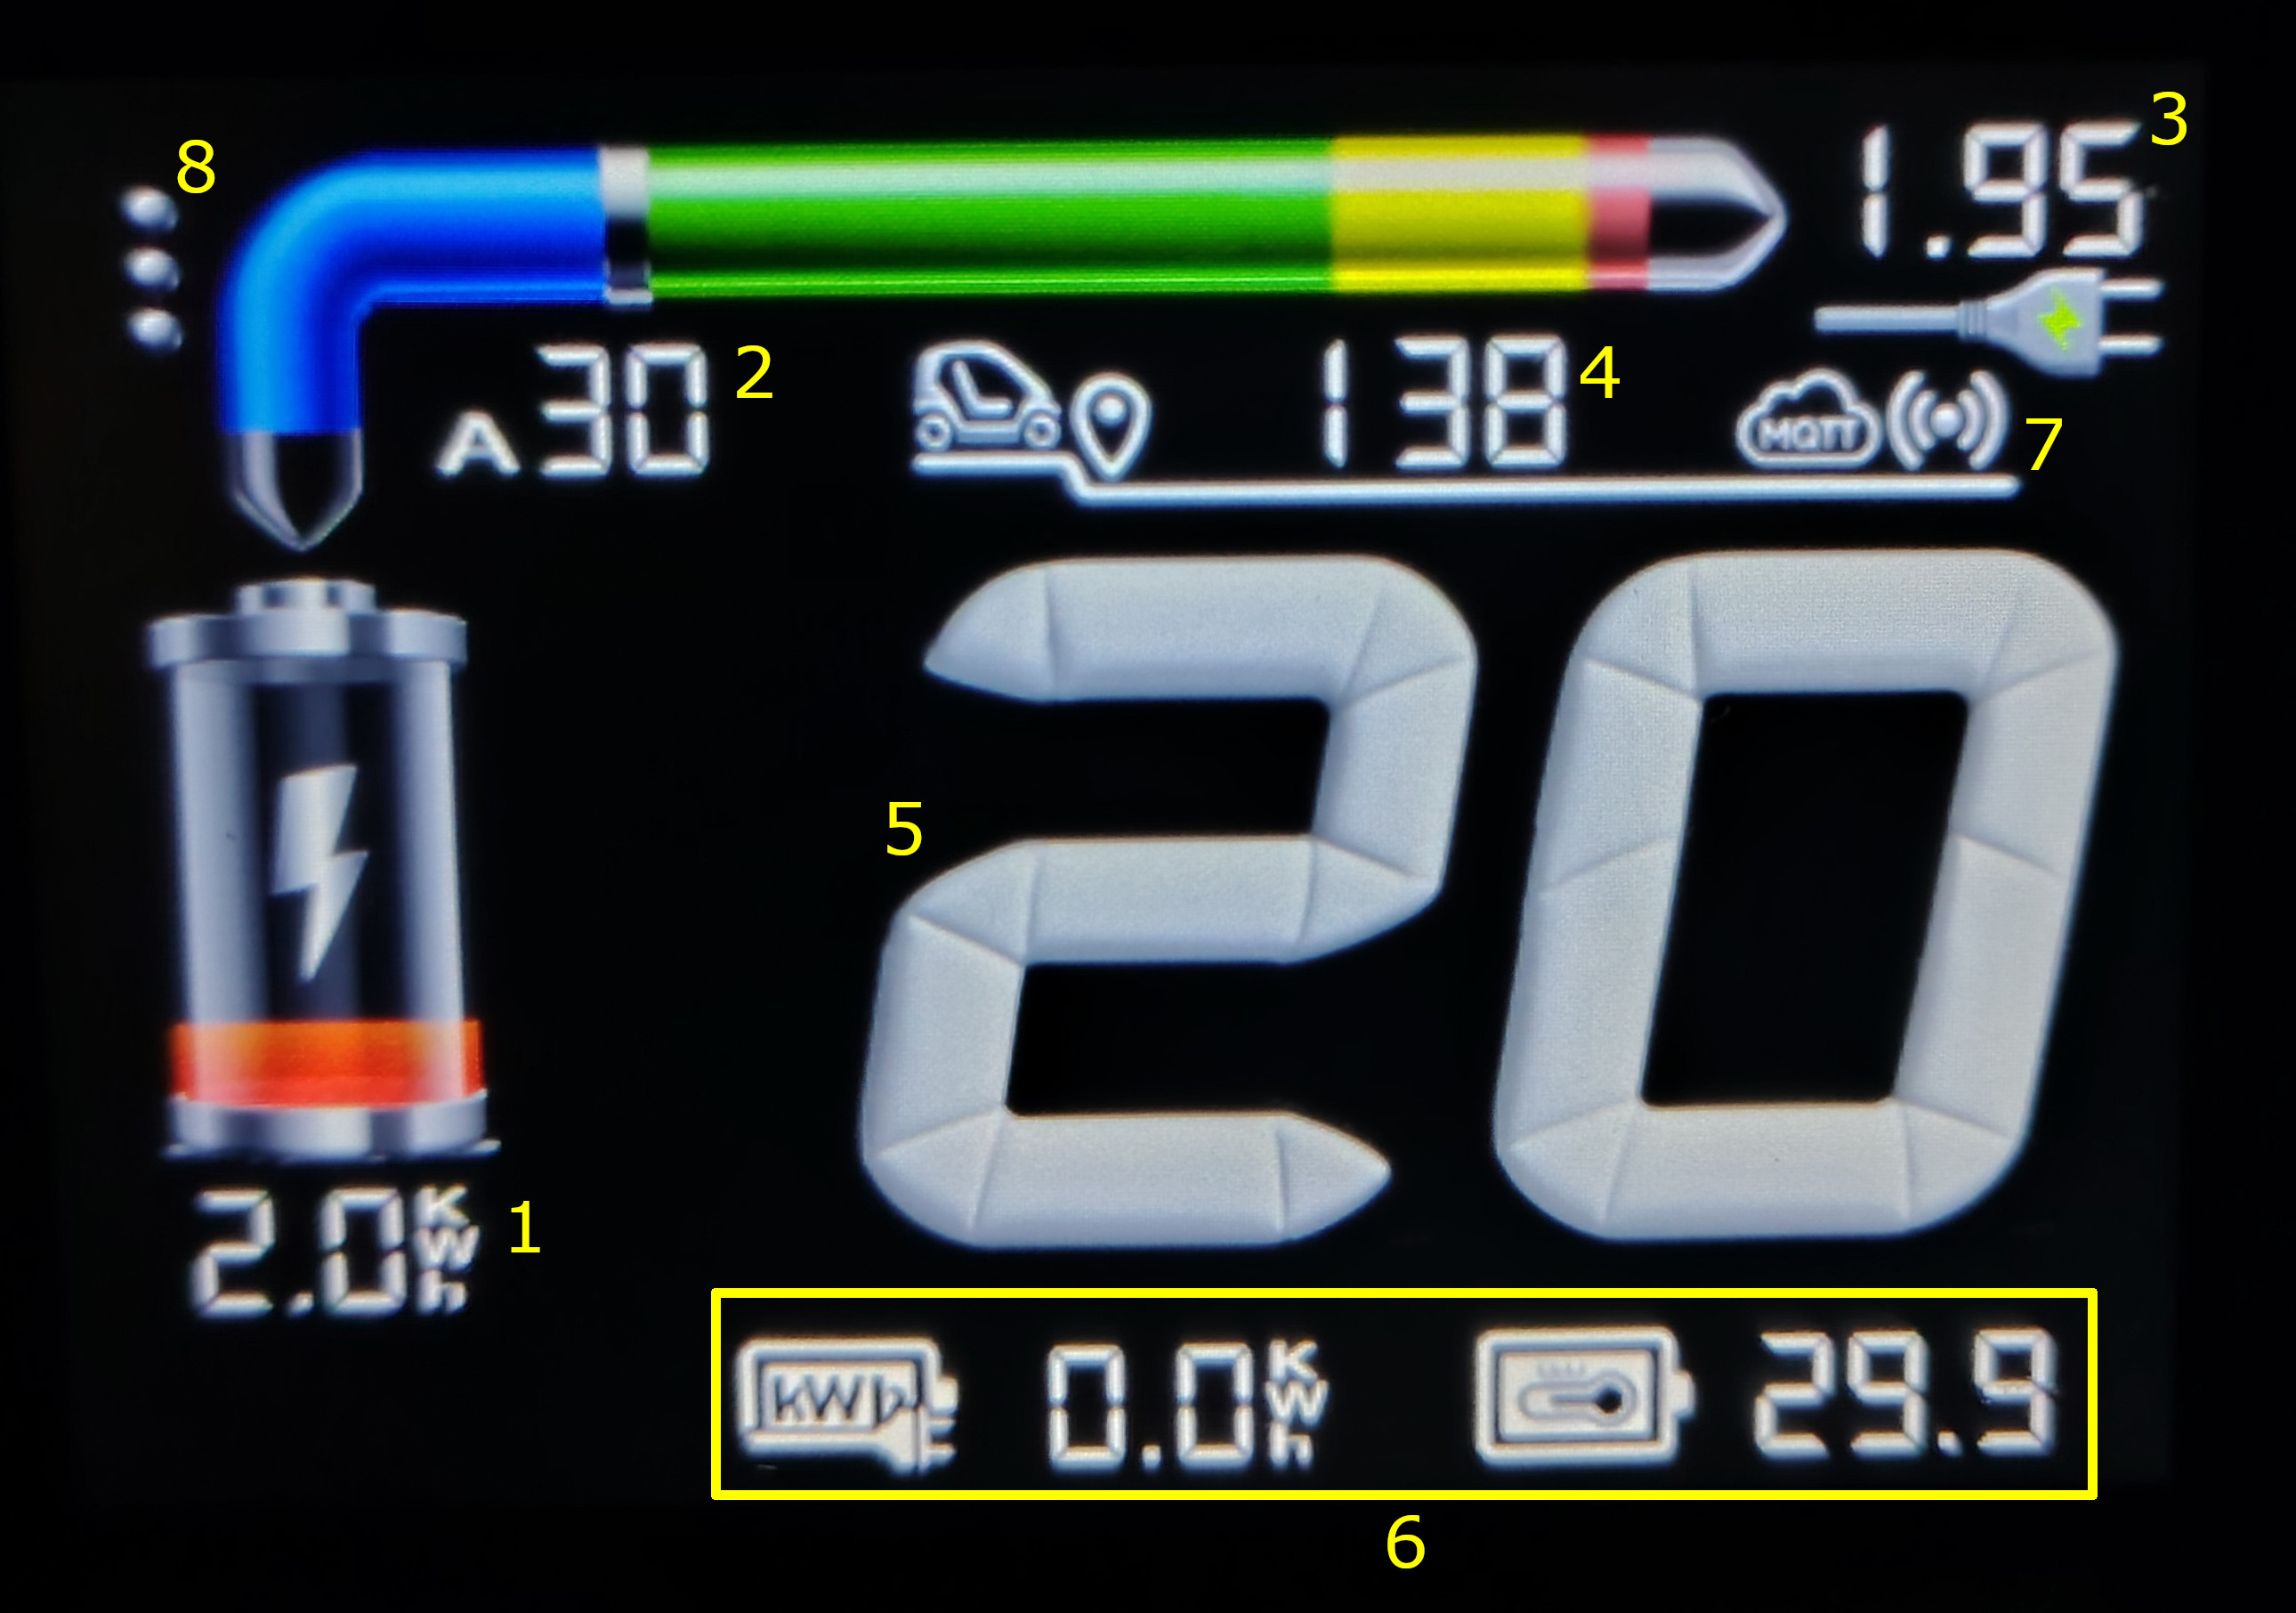
\includegraphics[width=0.8\textwidth]{figures/charging_page.jpg}
    \caption{Die Ladeseite.}
\end{figure}

\begin{description}
\item[\textbf{1}] Aktuell in der Batterie gespeicherte Leistung, ausgedrückt in \(kWh\).
\item[\textbf{2}] Ein Wert, ausgewählt aus Drehmoment, Stromverbrauch und Stromaufnahme, der verwendet wird, um
den blauen Teil des Leistungsbalkens zu füllen. Tippen Sie auf den Wert, um zwischen den drei Optionen zu wechseln.
\item[\textbf{3}] Aktuelle Ladeleistung, ausgedrückt in \(kW\), wird verwendet, um die rechte Seite des Leistungsbalkens zu füllen.
\item[\textbf{4}] Zeigt die ETA an, d. h. die geschätzte Zeit bis zum Abschluss des Ladevorgangs.
\item[\textbf{5}] Der aktuelle SOC, d. h. der Ladezustand der Batterie, ausgedrückt in \%.
\item[\textbf{6}] Zusätzlich angezeigte Werte, Sie können durch Antippen des Symbols zwischen ihnen wechseln.
\item[\textbf{7}] Symbole für MQTT und WiFi. Ausgegraut, wenn keine Verbindung besteht, und farbig bei Verbindung. Tippen Sie auf die Symbole, wenn Sie einen neuen WiFi-Scan oder eine MQTT-Neuverbindung durchführen möchten.
\item[\textbf{8}] Tastenkürzel zum Öffnen der Einstellungsseite für den Zugriff auf erweiterte Einstellungen.
\end{description}


\section{Die Einstellungsseite}
\label{sec:settings_page}

Um ToM wesentlich besser anpassbar zu machen, gibt es hier die Einstellungsseite, auf die durch
Drücken der drei Punkte in der oberen rechten Ecke auf einer der Hauptseiten zugegriffen werden kann. Jetzt können
Sie das grundlegende Erscheinungsbild Ihres persönlichen ToM leicht bearbeiten.

\begin{figure}[H]
    \centering
    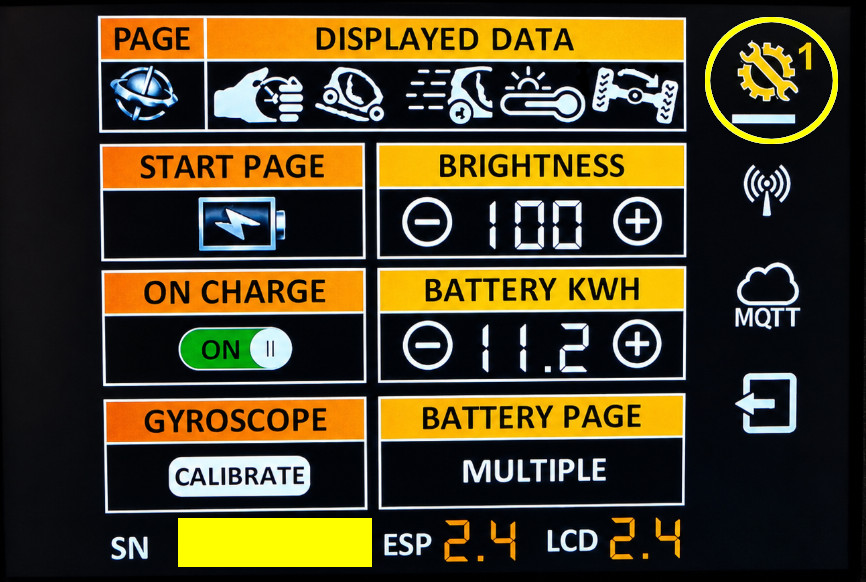
\includegraphics[width=0.8\textwidth]{figures/settings_page1.jpg}
    \caption{Die erste Einstellungsseite.}
    \label{fig:settings_page}
\end{figure}


\noindent Die letzte Zeile gibt Ihnen Informationen über Ihren persönlichen ToM und zeigt an:
\begin{itemize}
    \item Ihre ToM-\textbf{Seriennummer} im ersten Feld (im obigen Bild zensiert)
    \item Die Firmware-Version der Blackbox (ESP) (derzeit 2.4 im Bild)
    \item Die Firmware-Version des LCD-Touch-Displays (derzeit 2.4 im Bild)
\end{itemize}
Sie können auf die neueste Version der Firmware aktualisieren, wie in Abschnitt~\ref{sec:update_procedure} beschrieben.


\subsection{Erste Einstellungsseite}

Wie Sie auf dem obigen Bild vielleicht bemerken, wird Ihnen die eingekreiste Schaltfläche in der oberen rechten Ecke sagen,
auf welcher Einstellungsseite Sie sich gerade befinden. In diesem Fall ist es die erste, aber Sie können sie drücken, um
zur zweiten zu wechseln. Die erste Seite befasst sich hauptsächlich mit dem Erscheinungsbild des ToM+, während die zweite Seite sich mit dem Verhalten des ToM+ und einigen anderen erweiterten Einstellungen befasst.

\subsubsection{Anpassen der Seitenwerte}

Wenn Sie die Reihenfolge der auf einer Seite angezeigten Daten ändern oder sogar Daten von verschiedenen Seiten kombinieren möchten,
können Sie dies auf der Einstellungsseite tun, indem Sie diesen Schritten folgen.

\begin{figure}[H]
    \centering
    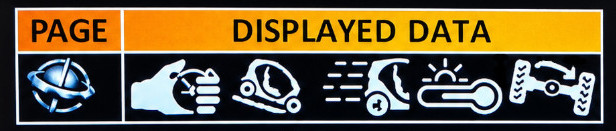
\includegraphics[width=0.8\textwidth]{figures/settings_page1_values.jpg}
    \caption{Anpassen der Seitenwerte.}
\end{figure}

Durch Drücken auf das erste Symbol durchlaufen Sie alle verfügbaren Seiten, deren Symbole 
zuvor in Abschnitt~\ref{sec:page_icon_list} erklärt wurden, und Sie können die Werte für diese bestimmte Seite anpassen.
Im obigen Bild hat der Benutzer die Gyroskop-Seite ausgewählt, sodass die auf der rechten Seite angezeigten Werte die aktuell für diese Seite festgelegten sind.\\

Jedes der fünf Symbole unter der Überschrift \textbf{Displayed Data} (Angezeigte Daten) kann durch Antippen angepasst werden, wobei alle Daten durchlaufen werden, bis Sie die gewünschte gefunden haben (Symbolbedeutung in Abschnitt~\ref{sec:icon_list} erklärt).
Zum Beispiel können Sie auch wählen, einige Motordaten auf der Batterieseite anzuzeigen und die beiden zu kombinieren.\\

\begin{figure}[H]
    \centering
    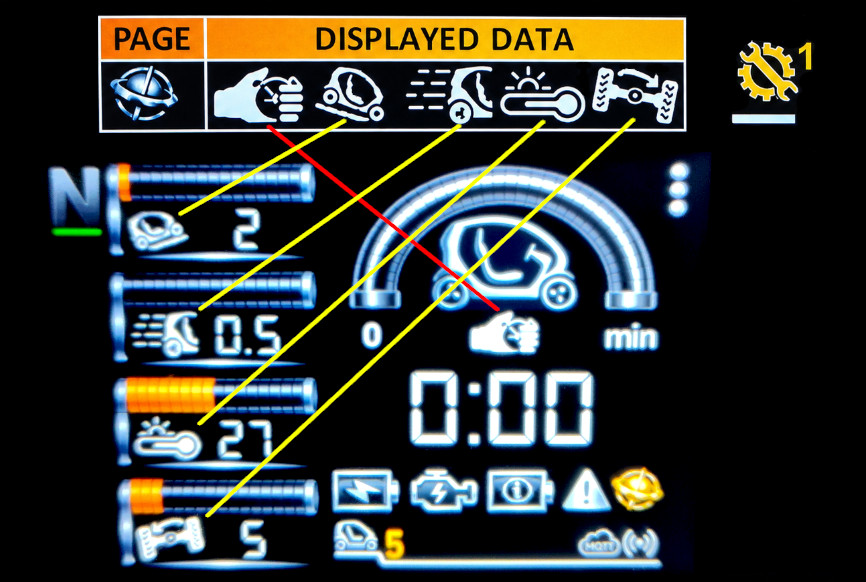
\includegraphics[width=0.8\textwidth]{figures/settings_page1_matching.jpg}
    \caption{Resultierende Layoutwerte.}
    \label{fig:icon_arrangement}
\end{figure}

Nachdem Sie die angezeigten Werte angepasst haben, \textbf{denken Sie daran, sie zu speichern, indem Sie auf die Schaltfläche Beenden drücken}.
Die neue Konfiguration wird wie im Bild gezeigt resultieren: Die erste Angabe wird im
Vordergrund in der Mitte der Seite angezeigt, während alle anderen
in der Tabelle auf der linken Seite in der auf der Einstellungsseite angegebenen Reihenfolge aufgelistet werden.

\subsubsection{Auswählen der Startseite}

Sie können wählen, welche Seite als erstes angezeigt wird, wenn Sie die Armaturenbrett-Seite verlassen.
Drücken Sie dazu auf das Symbol, um durch alle verfügbaren Seiten zu blättern, bis Sie die gewünschte finden.


Im Bild unten hat der Benutzer die Batterieseite ausgewählt, sodass das ToM+ diese zuerst anzeigt, wenn er die Armaturenbrett-Seite verlässt.\\

\begin{figure}[H]
    \centering
    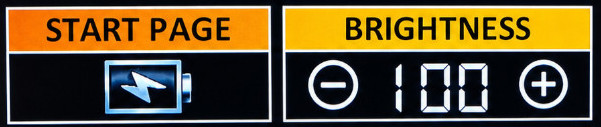
\includegraphics[width=0.8\textwidth]{figures/settings_page1_bright.jpg}
    \caption{Anpassen von Startseite und Helligkeit.}
\end{figure}

\subsubsection{Anpassen der Displayhelligkeit}

Wie Sie im obigen Bild sehen können, können Sie die Displayhelligkeit anpassen, indem Sie auf die Schaltflächen \texttt{-} oder \texttt{+} drücken.
Die Helligkeit kann von 0 bis 100 \% eingestellt werden und die Änderung wird sofort angewendet.\\

\subsubsection{Aktivieren/Deaktivieren der Ladeseite}

Das ToM+ verfügt über eine spezifische Seite zur Anzeige speziellerer Ladedaten (Abschnitt~\ref{sec:charging_page}). Sie können wählen,
ob Sie sie aktiviert (\textit{vertrauen Sie mir, es lohnt sich!}) oder deaktiviert lassen möchten.


Tippen oder schieben Sie den Schalter links, um zwischen ON und OFF zu wählen. Wenn der Schiebeschalter
auf ON eingestellt ist, startet das ToM und lädt die Ladeseite, wenn Ihr Twizy lädt, ansonsten,
im Zustand OFF, ist es während des Ladevorgangs ausgeschaltet. Um Ihre
Änderungen zu speichern, drücken Sie die Beenden-Schaltfläche in der unteren rechten Ecke.\\

\begin{figure}[H]
    \centering
    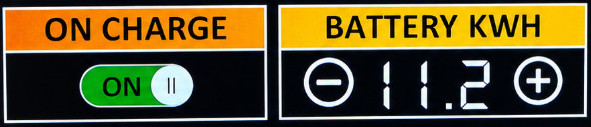
\includegraphics[width=0.8\textwidth]{figures/settings_page1_charge.jpg}
    \caption{Anpassen der Ladeseite und Batterie-kWh.}
\end{figure}

\subsubsection{Einstellen Ihrer Batteriekapazität}

Sie können Ihre Batteriekapazität in kWh einstellen, was nützlich ist, wenn Sie einen Twizy mit einer anderen
Batterie als der Standardbatterie haben. Dies hilft dem ToM+, die verbleibende Reichweite genauer zu berechnen.
Sie können den Wert in Schritten von 0,1 kWh anpassen, indem Sie auf die Schaltflächen \texttt{-} oder \texttt{+} drücken, und die Änderung wird sofort angewendet.
Stellen Sie sicher, dass Sie \textbf{Ihre neue Konfiguration speichern}, indem Sie die Beenden-Schaltfläche in der unteren rechten Ecke drücken.

\subsubsection{Kalibrierung des Gyroskopmoduls}

Wenn Sie feststellen, dass die Neigungsdaten des Gyroskops möglicherweise falsch sind, versuchen Sie,
die Schaltfläche „CALIBRATE“ (KALIBRIEREN) zu drücken, die eine Gyroskopkalibrierung durchführt. Stellen Sie sicher, dass
Sie sich mit Ihrem Twizy \textbf{auf einer ebenen Fläche} befinden, bevor Sie diesen Vorgang durchführen, da Ihre
Neigungsdaten andernfalls noch schlechter wären. Der Vorgang ist hier unten abgebildet:

\begin{figure}[H]
    \centering
    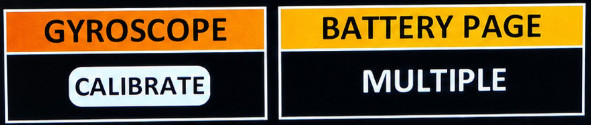
\includegraphics[width=0.8\textwidth]{figures/settings_page1_calibrate.jpg}
    \caption{Anpassen der Gyroskopkalibrierung.}
\end{figure}

\subsubsection{Ändern des Batterieseitenmodus}

Sie können auswählen, ob nur die komprimierte Batterie-Info-Seite (Abschnitt~\ref{sec:condensed_binfo}) angezeigt werden soll, wenn Sie auf die Schaltfläche Batterie-Info drücken, oder nicht.

Die beiden verfügbaren Optionen sind \textit{'Condensed'} (Komprimiert) und \textit{'Multiple'} (Mehrfach) und Sie können
zwischen ihnen wechseln, indem Sie auf den Text drücken. Die Änderung wird übernommen, sobald Sie die Beenden-Schaltfläche in der unteren rechten Ecke drücken.
Der Modus \textbf{Multiple} zeigt alle vier Batterieseiten an, die wir in Abschnitt~\ref{sec:condensed_binfo} besprochen haben,
während der Modus \textbf{Condensed} nur die komprimierte Seite anzeigt.\\

\subsection{Zweite Einstellungsseite}

Diese zweite Einstellungsseite befasst sich mit einigen erweiterten Einstellungen zum Ladevorgang. 
Um darauf zuzugreifen, drücken Sie die eingekreiste Schaltfläche in der oberen rechten Ecke der ersten Einstellungsseite und
drücken Sie sie erneut, um zur ersten Einstellungsseite zu navigieren.\\

\begin{figure}[H]
    \centering
    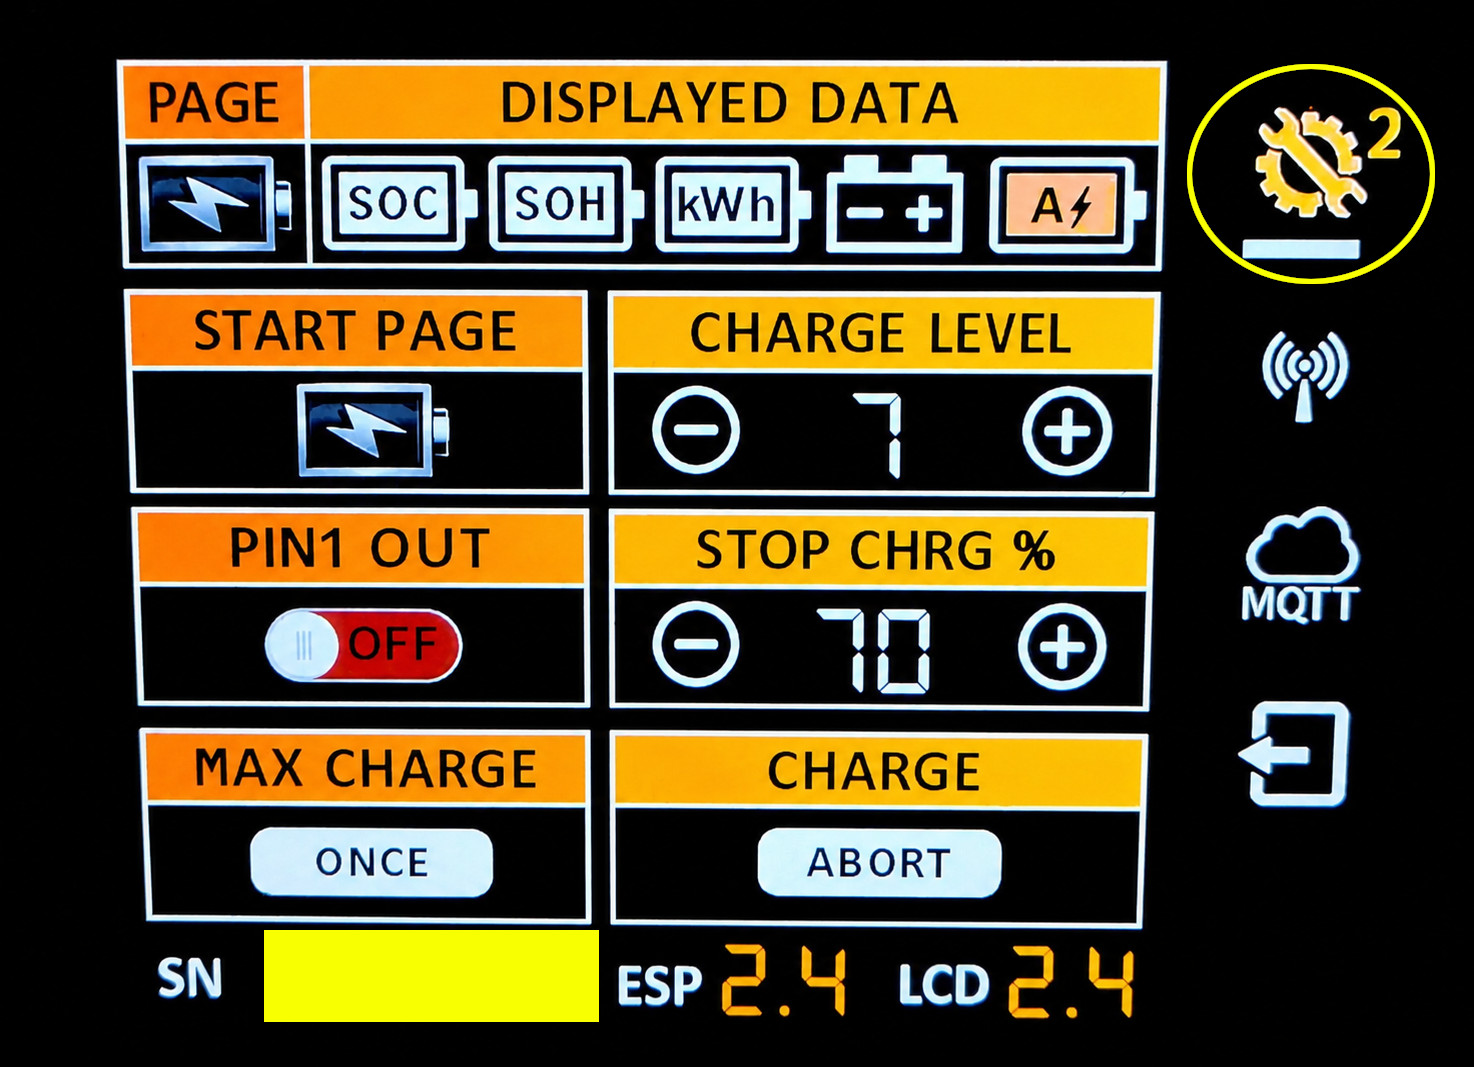
\includegraphics[width=0.8\textwidth]{figures/settings_page2.jpg}
    \caption{Zweite Einstellungsseite.}
\end{figure}

\subsubsection{Ändern des Ladezustands}

Sie können den maximalen Ladezustand Ihrer Twizy-Batterie wählen, was nützlich ist, wenn Sie
die von der Batterie aufgenommene Leistung begrenzen möchten, um ihre Lebensdauer zu erhöhen oder für andere Zwecke.
Die Stufe \textit{'0'} bedeutet, dass der Begrenzer deaktiviert ist, während die Stufen \textit{'1'} bis \textit{'7'} bedeuten, dass die entsprechende Ladestufe bis zum verfügbaren Maximum verwendet wird. 

Um die Stufe zu erhöhen oder zu verringern, drücken Sie auf die Schaltflächen \texttt{-} oder \texttt{+}.
Die Änderung wird auf die aktuelle Ladung angewendet, falls bereits geladen wird, oder auf die nächste Ladung, falls nicht.\\

\begin{figure}[H]
    \centering
    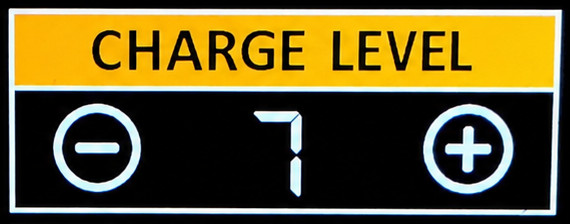
\includegraphics[width=0.6\textwidth]{figures/settings_page2_lvl.jpg}
    \caption{Ändern der Ladestufe.}
\end{figure}

\subsubsection{Manuelle Steuerung des Erweiterungs-PIN1}

Einige Benutzer gaben an, dass es nützlich wäre, eine manuelle Steuerung des Erweiterungs-PIN1 zu haben, der normalerweise zur Steuerung eines Zusatzladegeräts verwendet wird. Bei Bedarf können Sie den Erweiterungs-PIN1 also manuell steuern, indem Sie die EIN/AUS-Taste drücken.
Die Änderung wird übernommen, sobald Sie die Beenden-Schaltfläche in der unteren rechten Ecke drücken.\\

\begin{figure}[H]
    \centering
    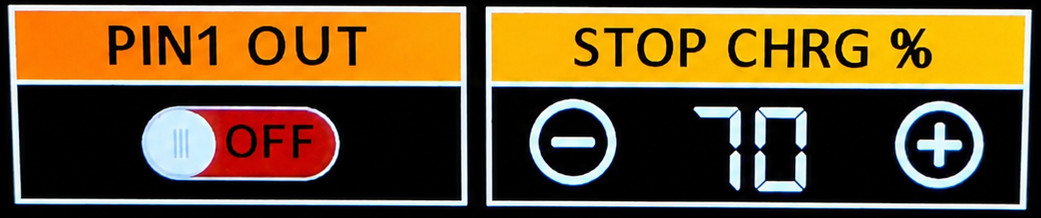
\includegraphics[width=0.8\textwidth]{figures/settings_page2_stop.jpg}
    \caption{Manuelle Steuerung des Erweiterungs-PIN1 und Stopp-Ladestufe.}
\end{figure}

\subsubsection{Stoppen der Ladung bei einem bestimmten SOC}

Sie können wählen, den Ladevorgang bei einem bestimmten SOC zu stoppen, was nützlich ist, wenn Sie die Batterielebensdauer verlängern möchten. Sie können den Wert von 0 bis 100 \% einstellen, indem Sie auf die Schaltflächen \texttt{-} oder \texttt{+} drücken.
Die Änderung wird auf die aktuelle Ladung angewendet, falls bereits geladen wird, oder auf die nächste Ladung, falls nicht.\\

\subsubsection{Durchführung einer Ladung mit maximalen Parametern}

Sie können wählen, eine Ladung ohne Leistungs- und SOC-Grenzen durchzuführen, was nützlich ist, wenn Sie ab und zu die Batteriezellen ausgleichen möchten. Sie können die Schaltfläche drücken, um die Ladung mit maximalen Parametern zu starten, die auf die aktuelle Ladung angewendet wird, falls bereits geladen wird, oder auf die nächste Ladung, falls nicht.\\

\begin{figure}[H]
    \centering
    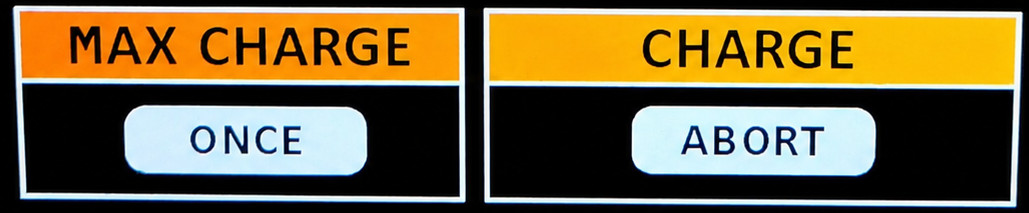
\includegraphics[width=0.8\textwidth]{figures/settings_page2_max.jpg}
    \caption{Ladung mit maximalen Parametern und Ladevorgang abbrechen.}
\end{figure}

\subsubsection{Ladevorgang abbrechen}

Sie können wählen, den Ladevorgang abzubrechen, was nützlich ist, wenn Sie den Ladevorgang sofort stoppen möchten.
Sie können die Schaltfläche drücken, um den Ladevorgang abzubrechen, was sofort ausgeführt wird.\\

\clearpage

\subsection{Das rechte Seitenmenü}

\iconbox{icons/SetupRed1.png}
{Einstellungsseite (1 oder 2)}
{Zeigt an, auf welcher Einstellungsseite Sie sich befinden. Klicken Sie zum Wechseln.}

\iconbox{icons/WifiBianco.PNG}
{WiFi-Einstellungsseite}
{Seite zu den WiFi-Einstellungen wechseln. (Abschnitt~\ref{sec:wifi_settings})}

\iconbox{icons/MQTTBianco.PNG}
{MQTT-Einstellungsseite}
{Seite zu den MQTT-Einstellungen wechseln. (Abschnitt~\ref{sec:MQTT})}

\iconbox{icons/ExitIcon2.png}
{Speichern und Beenden-Schaltfläche}
{Änderungen speichern und zur letzten Seite zurückkehren.}
